\documentclass[a4paper,14pt,oneside,openany]{memoir}
\usepackage[left=2.5cm, right=1cm, top=2cm, bottom=2cm]{geometry}

\usepackage[backend=biber,style=numeric,sorting=none]{biblatex}
\DeclareFieldFormat{labelnumberwidth}{{#1\adddot}}
  
\usepackage{bm}
\usepackage{amsmath}
\usepackage{amssymb}
\usepackage[russian]{babel}
\renewcommand{\baselinestretch}{1.5}
\setlength{\parindent}{1.25cm}
\usepackage{indentfirst}
\usepackage[utf8]{inputenc}
\usepackage{csquotes}
\usepackage{verbatim} % multi comments

%% pics, tables
\usepackage{graphicx}
\usepackage{caption}
\captionsetup[figure]{name={Рисунок}, labelsep={space}, justification=centering}
\captionsetup[table]{labelsep={space}}
\graphicspath{ {./pics/estcmpr/} {./pics/lims/} {./pics/mau/}, {./pics/observer/}, {./pics/acsl/}, {./pics/}}
\usepackage{subfig}
\usepackage{float}

%% sections style
\usepackage{titlesec}
\titleformat*{\section}{\normalfont\bfseries}

%% page style
\pagestyle{myheadings} % нумерация страниц вверху справа
\aliaspagestyle{chapter}{myheadings} % нумерация страниц вверху справа
\renewcommand{\cftchapterpagefont}{\normalfont}% нежирные номера страниц у глав в оглавлении
\renewcommand{\cftchapterleader}{\cftdotfill{\cftchapterdotsep}}% нежирные точки до номеров страниц у глав в оглавлении
\renewcommand{\cftchapterfont}{}% нежирные названия глав в оглавлении

\addbibresource{bibliography/citations.bib}

\begin{document}
	\thispagestyle{empty}
\begin{comment} 
«Федеральное государственное бюджетное образовательное\\
учреждение высшего образования \\
«Московский авиационный институт \\
(национальный исследовательский университет)»
\end{comment}

\begin{center} 
«Федеральное государственное автономное образовательное учреждение высшего образования «Московский физико-технический институт (национальный исследовательский университет)»
\end{center}

{
\vskip 5mm
}

\begin{flushright}
На правах рукописи
\end{flushright}


{
   	\vskip 12mm
}

\begin{center}
	Шавин Михаил Юрьевич
\end{center}
\begin{center} 
	\textbf{«РАЗРАБОТКА МЕТОДОВ УПРАВЛЕНИЯ И МОДЕЛИРОВАНИЕ ДИНАМИКИ КВАДРОКОПТЕРА С ПОВОРОТНЫМИ РОТОРАМИ»} \\
	Специальность: 05.07.09 \\
	Динамика, баллистика, управление движением летательных аппаратов
\end{center}

{
	\vskip 6mm
}

\begin{center} 
	Диссертация \\
	на соискание ученой степени \\
	кандидата технических наук
\end{center}


{
	\vskip 12mm
}

\begin{center} 
Научный руководитель: \\
кандидат физико-математических наук, доцент, \\ 
Притыкин Дмитрий Аркадьевич, \\
старший научный сотрудник Космического центра Сколтеха \\
\vspace{5mm}
%$\rule{102mm}{0.15mm}$
\end{center}

{
	\vskip 8mm
}

\begin{center} 
Москва -- 2020
\end{center}

	\tableofcontents
	
\chapter{Общая характеристика диссертации}

\section{Актуальность темы исследования}

Беспилотные летательные аппараты (БЛА) мультироторного типа находят все более широкое применение в различных областях деятельности, а миниатюризация и доступность электронных компонентов их бортового оборудования приводит к расширению спектра задач, в решении которых используются такие аппараты.
Интерес исследователей к БЛА обусловлен также и тем, что они являются доступным средством для отработки новых технологий в аэрокосмической отрасли \cite{Otero01}.

С момента создания первых квадрокоптеров интенсивно ведутся исследования в области их динамики и управления, причем количество работ растет с каждым годом, что можно наблюдать по динамике количества публикаций (рис. \ref{pic:res_amount}), посвященных квадрокоптерам, доступных на крупнейшей онлайн платформе научных публикаций «Google Академия».
Однако, несмотря на обилие публикаций в области управляемой динамики квадрокоптеров, остаются перспективные направления, среди которых усовершенствование конструкции БЛА, связанное с увеличением размерности вектора управляющих воздействий.
Конструктивно это достигается, например, с помощью сервоприводов, способных поворачивать роторы с пропеллерами относительно корпуса.
\begin{figure}[h!]
	\centering
	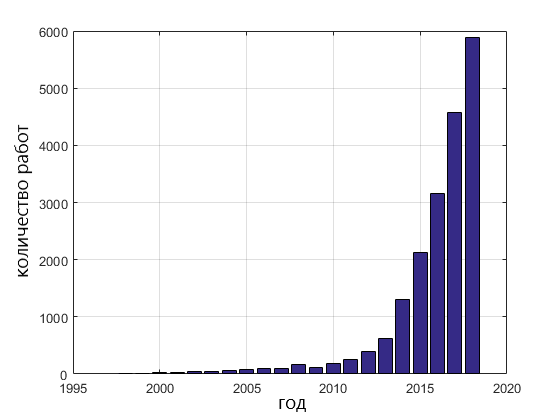
\includegraphics[width=0.95\columnwidth]{res_amount}
	\caption{ -- Динамика количества публикаций, посвященных квадрокоптерам}
	\label{pic:res_amount}
\end{figure}
{
	\vskip 5mm
}

Стандартный квадрокоптер с четырехмерным вектором управляющих воздействий и шестью степенями свободы корпуса аппарата не способен, например, независимо управлять положением и ориентацией.
Это приводит к необходимости дополнительных устройств для наведения камер или лазерных дальномеров, используемых при выполнении ряда стандартных для БЛА задач.
Возможность независимо управлять положением и ориентацией, приобретаемая за счет использования поворотных роторов, влияет не только на работу полезной нагрузки и датчиков, но и на функциональные возможности всей системы в целом.
Согласно работе \cite{Stolc01}, усовершенствованные таким образом квадрокоптеры более устойчивы к возмущениям внешней среды, а также лучше стандартных квадрокоптеров пригодны для вертикального взлета и посадки на неровные поверхности.

Достоинства БЛА с поворотными роторами отмечают и исследователи, работающие над управлением БЛА в экстренных ситуациях (при отказе части двигателей) \cite{Morozov01, Shidar00}.
В работе \cite{Shidar00} обосновывается достижение более высокой скорости за счет выбора оптимальной по отношению к набегающему потоку ориентации, а также более рациональное, по сравнению со стандартными аппаратами, энергопотребление.
В работе \cite{Morozov01} отмечена перспективность конструкции с поворотными роторами, однако ее применение не рассматривается из-за сложности реализации.
Использование поворотных роторов действительно усложняет реализацию контура управления \cite{Ryll01, Falconi01, Segui01, Oosedo01} и не позволяет применять ставшую классической, изящную схему управления \cite{Mellinger01}, однако, есть основания полагать, что предлагаемое в работе аналитическое обращение динамики системы позволит преодолеть некоторую часть возникающих трудностей.

\section{Цели и задачи исследования}

Объектом исследования является система управления движением квадрокоптера с поворотными роторами, предметом исследования -- динамика и методы управления движением квадрокоптера с поворотными роторами.

Цель работы -- выполнить анализ динамики квадрокоптера с поворотными роторами;
разработать алгоритмы управления движением квадрокоптера с поворотными роторами для выполнения различных маневров; разработать алгоритмы управления движением квадрокоптера с поворотными роторами для экстренного сценария -- потере двух смежных двигателей. Для достижения цели работы необходимо решить следующие задачи:
\begin{enumerate}
	\item Разработать математическую модель движения квадрокоптера с поворотными роторами с учетом сил и моментов, действующих на все составные части системы.
	\item Решить задачу обратной динамики и синтезировать контур управления квадрокоптером с поворотными роторами для независимого управления положением и ориентацией аппарата с учетом физических ограничений, накладываемых на исполнительные органы системы управления.
	\item Разработать алгоритмы для идентификации аэродинамических параметров пропеллеров.
	\item Обеспечить обратную связь в контуре управления, реализовать алгоритмы оценки состояния на основе фильтра Калмана.
	\item Реализовать алгоритмы управления квадрокоптером с поворотными роторами в случае аварийного отказа  двигателей, позволяющие аппарату выполнение номинальных задач.
\end{enumerate}
Для решения сформулированных задач используются классические методы механики, управления, вычислительной и высшей математики.

Область исследования соответствует пунктам «Баллистическое проектирование летательных аппаратов различного назначения» и «Динамическое проектирование управляемых летательных аппаратов и исследование динамики их движения» паспорта специальности «05.07.09 – Динамика, баллистика, управление движением летательных аппаратов».

\section{Положения, выносимые на защиту}
Положения, выносимые на защиту:
\begin{enumerate}
	\item Математическая модель управляемой динамики квадрокоптера с поворотными роторами с учетом сил и моментов, действующих на все составные части системы.
	\item Синтез контура управления квадрокоптером с поворотными роторами на основе решения обратной задачи динамики для независимого управления положением и ориентацией аппарата.
	\item Алгоритм для учета физических ограничений, накладываемых на исполнительные органы системы управления.
	\item Алгоритм идентификации аэродинамических параметров пропеллеров.
	\item Алгоритмы оценки состояния квадрокоптера с поворотными роторами.
	\item Алгоритм экстренного управления квадрокоптером с поворотными роторами в случае отказа смежных двигателей.
	\item Выводы и рекомендации, сформулированные в работе.
\end{enumerate}

\section{Степень достоверности и апробация результатов}
Достоверность полученных научных положений, результатов и выводов обеспечивается
соответствием выбранных моделей движения общепринятым стандартам,
адекватностью выбранных методов исследования движения,
проведением численного моделирования полученных аналитических результатов,
а также сопоставлением с результатами,
полученными другими авторами для частных случаев рассматриваемых задач.

Основные научные положения и результаты работы докладывались и обсуждались на 
\begin{itemize}
	\item Всероссийской конференции молодых ученых-механиков, 5 - 15 сентября 2017 г., г. Сочи, «Буревестник» МГУ;
	\item Международной научной конференции «Фундаментальные и прикладные задачи механики», 24 - 27 октября 2017 г., г. Москва;
	\item 60-й Всероссийской научной конференции МФТИ, секция теоретической механики, 20–26 ноября 2017 г., г. Долгопрудный;
	\item 60-й Всероссийской научной конференции МФТИ, секция управления динамическими системами, 20–26 ноября 2017 г., г. Москва;
	\item седьмой международной конференции «Geometry, Dynamics, Integrable Systems», 5-9 июня 2018 г., г. Москва;
	\item XIV Международной конференции «Устойчивость и колебания нелинейных систем управления» (конференция Пятницкого) Россия, Москва, ИПУ РАН, 30 мая -- 1 июня 2018 г.
	\item 14-ой международной конференции «Vibration engineering and technology of machinery», 10-13 сентября 2018 г., г. Лиссабон, Португалия;
	\item Международной конференции «Проблемы механики и управления», 16-22 сентября 2018 г., г. Махачкала;
	\item XXI конференции молодых ученых «Навигация и управление движением», 19–22 марта 2019 г., г. Санкт-Петербург.
	\item XII Всероссийский съезд по фундаментальным проблемам теоретической и прикладной механики, 9 -- 24 августа 2019 г., г. Уфа.
\end{itemize}
По теме исследования были опубликованы 15 работ, в том числе 2 в журналах, рекомендованных ВАК РФ, 2 в журналах, входящих в базу данных SCOPUS, 1 полезная модель к патенту и 3 патентных свидетельства. Cписок можно найти на странице \pageref{list_chapter}.

\section{Научная новизна и практическая значимость работы}
Научная новизна представленных в диссертации результатов заключается в следующем:
\begin{enumerate}
	\item  Разработана математическая модель движения квадрокоптера с поворотными роторами, получено аналитическое решение задачи обратной динамики БЛА.
	\item Синтезирован контур управления квадрокоптером с поворотными роторами на основе решения обратной задачи динамики для независимого управления положением и ориентацией аппарата.
	\item  Проведен анализ аналитического решения задачи обратной динамики  БЛА с поворотными роторами; разработан алгоритм реализации ограничений на компоненты вектора управляющих воздействий, позволяющий учесть физические ограничения исполнительных органов системы управления.
	\item Разработан алгоритм идентификации аэродинамических параметров пропеллеров на основе расширенного фильтра Калмана.
	\item Исследована производительность различных алгоритмов нелинейной фильтрации для оценки состояния БЛА с поворотными роторами.
	\item Разработан алгоритм экстренного управления квадрокоптером с поворотными роторами в случае отказа  смежных двигателей.
\end{enumerate}

Практическая значимость работы состоит в том, что
реализация разработанной в исследовании системы управления позволяет проектировать БЛА с улучшенными относительно стандартных квадрокоптеров летными характеристиками, в том числе обладающих способностью 
выполнять сложные маневры, недоступные стандартным квадрокоптерам, такие, как маневры с требованием независимого управления положением и ориентацией.
Таким образом, расширяются возможности беспилотных летательных аппаратов.
Кроме этого, реализованная в программных алгоритмах динамическая модель и система управления позволяет на предварительном этапе проектирования БЛА определить параметры регулятора и динамики мультироторного робота в зависимости от выбранных комплектующих и других факторов.

\section{Личный вклад автора}
Все результаты, вынесенные на защиту, получены автором самостоятельно.
Также автором самостоятельно проведены численные эксперименты,
подтверждающие основные положения и выводы работы.
	

\chapter{Обзор литературы} \label{review}
\section{Летательные аппараты мультироторного типа} \label{review_s1}

История развития летательных аппаратов мультироторного типа началась более ста лет назад, когда братья Бриджет и профессор Ричет создали конструкцию, которую назвали Гироплан №1 \cite{Leishman02, Leishman01}. Осенью 1907 года их гироплан вместе с пилотом на борту оторвался от земли менее чем на метр, продемонстрировав практическую возможность использования конструкции такого типа. С тех пор интерес исследователей к мультикоптерам постепенно возрастал и в настоящее время находится на очень высоком уровне во многом благодаря развитию технологий производства комплектующих для аппаратов такого типа и значительному уменьшению габаритов и массы бортовой вычислительной техники и датчиков, необходимых для построения автономной системы управления. Из-за простоты конструкции, маневренности, относительной доступности и дешевизны особенной популярностью сейчас пользуются квадрокоптеры -- беспилотные летательные аппараты мультироторнного типа с четырьмя двигателями. Эти преимущества позволяют использовать такие аппараты как инструмент для отработки новых подходов к построению систем управления и их тестированию, не ограничиваясь только лишь численными методами. Этот факт закономерно привел к тому, что на текущий момент существует достаточно большое количество работ, посвященных управляемой динамике беспилотных летательных аппаратов такого типа, значительно отличающихся по поставленным в иследованиях целям, применяемым методам и полученным результатам. В ряде публикаций предлагаются некоторые модификации конструкции стандартного квадрокоптера, которые позволяют повысить лётные характеристики беспилотного летательного аппарата (БЛА) и гарантируют некоторые другие преимущества перед квадрокоптерами стандартной конструкции. Ниже нами рассмотрены встречающиеся в современных публикациях основные подходы, посвященные проектированию систем управления как стандартных так и модифицированных конструкций БЛА, в основе которых лежат ПИД-регуляторы, линейно-квадратичные регуляторы, скользящие режимы управления, адаптивное управление, робастное управление и другие методы современной теории управления.

\section{Конструкция и основные принципы движения квадрокоптера}

Основными элементами конструкции стандартного квадрокоптера являются корпус и четыре двигателя с прикрепленными к ним пропеллерами. В зависимости от взаимного расположения двигателей и собственной оси продольного движения выделяют две стандартных схемы: \textit{cross}-схему и \textit{plus}-схему \cite{Bashi01} (см. рис. \ref{fig:cross_plus}).
\begin{figure}[h!]
	\centering
	\subfloat[Общий вид \textit{cross}-схемы]{%
		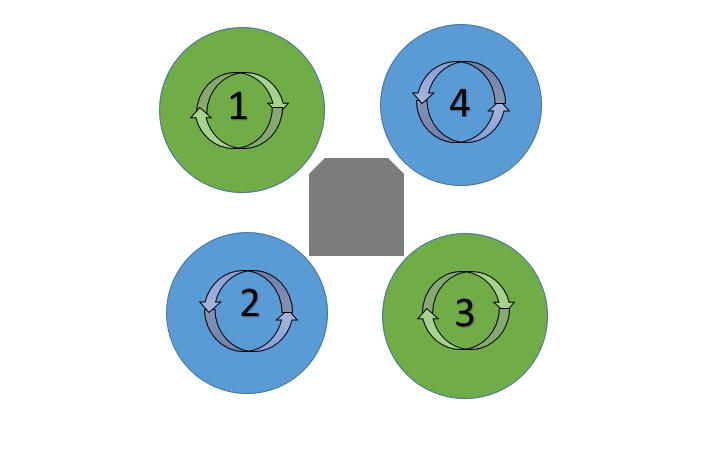
\includegraphics[width=0.44\columnwidth]{cross}%
	}
	\quad
	\subfloat[Общий вид \textit{plus}-схемы]{%
		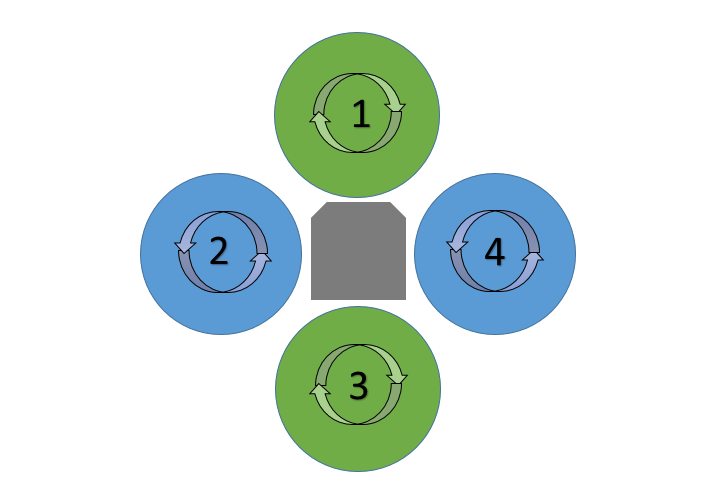
\includegraphics[width=0.44\columnwidth]{plus}%
	}
	\caption{ -- Основные схемы квадрокоптеров}
	\label{fig:cross_plus}
\end{figure}
Пропеллеры, расположенные на смежных лучах вращаются в разные стороны, благодаря чему возможна стабилизация по углу рысканья, при этом тяга каждого двигателя направленна одинаково. Вертикальное движение аппарата обусловлено изменением общей тяги всех двигателей. Горизонтальное движение совершается за счет изменения направления вектора тяги вследствие наклона корпуса БЛА \cite{Salih01}. 

\section{Основные подходы к построению модели динамики квадрокоптера}
	
Обычно, поступательное движение малых беспилотных летательных аппаратов рассматривают в инерциальной системе координат (назовем её {$I$}), связанной с поверхностью Земли. С учетом относительно небольших характерных расстояний и времен полета БЛА движением и кривизной поверхности Земли принебрегают.

Существуют два наиболее распространенных способа связать координатные оси с Землей: {$NED$} --  ось \textbf{$X_I$} направлена на север, ось \textbf{$Y_I$} -- на восток, а ось \textbf{$Z_I$} -- к центру Земли; {$ENU$} -- ось \textbf{$X_I$} направлена на восток, ось \textbf{$Y_I$} -- на север, а ось \textbf{$Z_I$} -- от центра Земли. Положение БЛА описывается радиус-вектором центра масс аппарата \bm{$r_I$},записанном в выбранной инерциальной системе координат. Скорость определяется, как
\begin{equation} \label{eq:velocity}
\bm{v_I} = \dot{\bm{r}}.
\end{equation}

Корпус квадрокоптера в рамках задачи управления движением обычно считают твердым телом. Для описания ориентации объекта в пространстве используют связанную с телом систему координат $B$, начало которой совпадает с центром масс БЛА, а оси направлены по главным центральным осям инерции корпуса (см. рис. \ref{fig:quad_scheme}). Текущее положение базиса B относительно I может быть описано матрицей поворота $\bm{R}_{IB}$, в том смысле, что разложения произвольного вектора $\bm{x}$, записанного в этих базисах, связаны соотношением
\begin{figure}[h!]
	\centering
	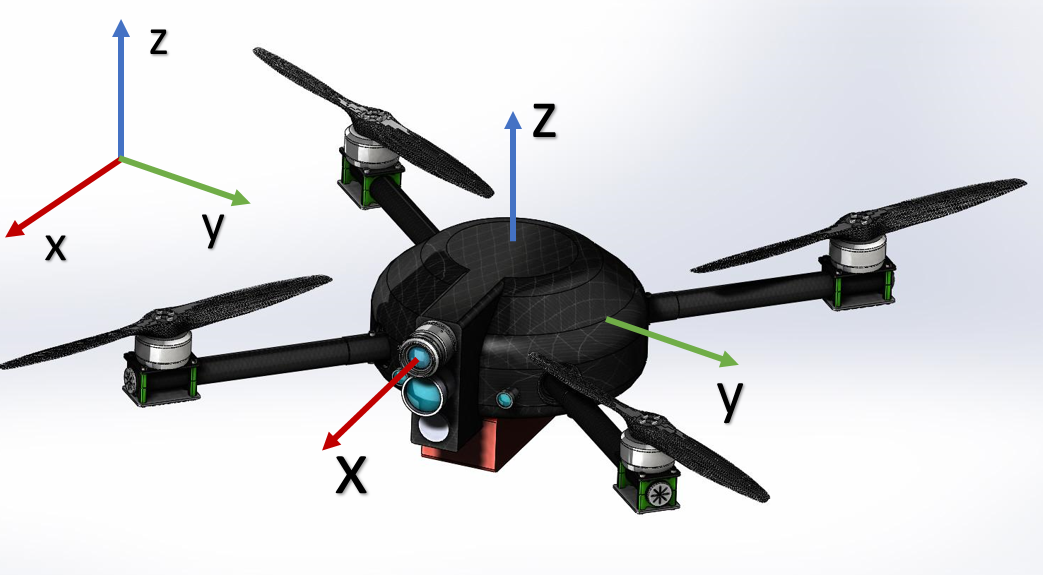
\includegraphics[width=0.9\columnwidth]{uavXYZ}
	\caption{ -- Квадрокоптер и системы кординат}
	\label{fig:quad_scheme}
\end{figure}
\begin{equation} \label{eq:rotmx}
\bm{x}_I = \bm{R}_{IB}\bm{x}_B.
\end{equation}
Матрица поворота связана с компонентами угловой $\bm{\Omega}_B$ скорости следующим соотношением
\begin{equation} \label{eq:angvel_rotmx}
\dot{\bm{R}}_{IB} = \bm{R}_{IB} [\bm{\Omega}_B]_{\times},
\end{equation}
где
\begin{equation} \label{eq:hat_operator}
[\bm{\Omega}]_{\times} =
\begin{bmatrix}
0            & -\bm{\Omega}^z   & \bm{\Omega}^y \\
\bm{\Omega}^z     & 0           &-\bm{\Omega}^x\\
-\bm{\Omega}^y    & \bm{\Omega}^x    & 0
\end{bmatrix}.
\end{equation}

Иногда для описания ориентации БЛА используют углы конечного поворота (иногда их называют углами Эйлера вне зависимости от последовательности), которые задают положение базиса B относительно базиса I через три  последовательных поворота вокруг осей связанной системы координат. Наиболее часто используются так называемые самолетные углы: последовательные повороты вокруг оси $Z_B$ на угол $\psi$, $Y_B$ на угол $\theta$, $X_B$ на угол $\phi$ будут определять углы рысканья, крена и тангажа. Им соответствует матрица поворота

\small
\begin{equation*} \label{eq:eul_to_rotmx}
\begin{aligned}
\bm{R} =
&\begin{bmatrix}
c(\psi)c(\theta) & c(\psi)s(\theta)s(\phi) - s(\psi)c(\phi) & c(\psi)s(\theta)c(\phi) + s(\psi)s(\phi) \\
s(\psi)c(\theta) & s(\psi)s(\theta)s(\phi) - c(\psi)c(\phi) & s(\psi)s(\theta)c(\phi) - c(\psi)s(\phi) \\
-s(\theta)         & c(\psi)s(\phi)                                 & c(\psi)c(\phi)\\
\end{bmatrix},
\end{aligned}
\end{equation*}
\normalsize
где для произвольного аргумента $x$ обозначим $c(x) = cos(x)$, $s(x) = sin(x)$. Обратное преобразование:
\begin{equation} \label{eq:rotmx_to_eul}
\begin{aligned}
&\psi  = \arctan\left( { - \frac{{{{\bm{R}}_{13}}}}{{{{\bm{R}}_{23}}}}} \right),
\\
\vspace{3mm}
\\
&{\theta  = \arccos  {{{\bm{R}}_{33}}} }
\\
\vspace{3mm}
\\
&\varphi  = \arctan\left( {\frac{{{{\bm{R}}_{31}}}}{{{{\bm{R}}_{32}}}}} \right)
\end{aligned}
\end{equation}

Помимо матриц и углов конечного поворота для описания ориентации часто используются кватернионы \cite{Amelkin01} -- четырехмерные гиперкомплексные числа, которые можно представить в виде формальной суммы скалярной и векторной частей
\begin{equation} \label{eq:quat_def}
Q = q_0 + \bm{q}.
\end{equation}
Для кватернионов определены операции сопряжения
\begin{equation} \label{eq:quat_dual}
\tilde{Q} = q_0 - \bm{q}
\end{equation}
и умножения
\begin{equation} \label{eq:quat_mult}
Q \circ P = q_0 p_0 - (\bm{q} \cdot \bm{p})
+ q_0 \bm{p} + p_0 \bm{q} + \bm{q} \times \bm{p}
\end{equation}
Кватернион ориентации  $q_{IB}$ определяет положение собственного базиса $B$ относительно базиса $I$ в том смысле, что разложения произвольного вектора $\bm{x}$, записанного в этих базисах, связаны соотношением
\begin{equation} \label{eq:quat}
\bm{x}_I = q_{IB} \circ \bm{x}_B \circ \tilde{q}_{IB}.
\end{equation}
Угловая скорость и кватернион ориентации связаны уравнением Пуассона
\begin{equation} \label{eq:puasson}
\dot{q}_{IB} = \frac{1}{2} {q}_{IB} \circ \bm{\Omega}_B.
\end{equation}
Кватернион ориентации эквивалентен матрице поворота
\begin{equation} \label{eq:quat_to_rotmx}
\bm{R} = ({q_0}^2 - \bm{q}^T \bm{q}) E_{3 \times 3} + 2 \bm{q}^T \bm{q} - 2 {q_0} [\bm{q}]_{\times},
\end{equation}
где $E_{n \times n}$ -- едичная матрица размерности $n$.
Его компоненты могут быть получены из углов Эйлера
\begin{equation}
\begin{aligned}
&{q_0} = \cos \frac{\theta }{2}\cos \frac{{\varphi  + \psi }}{2},
\\
\vspace{3mm}
\\
&{q_1} = \sin\frac{\theta }{2}\cos \frac{{\varphi  - \psi }}{2},
\\
\vspace{3mm}
\\
&{q_2} =  - \sin \frac{\theta }{2}\sin\frac{{\varphi  - \psi }}{2},
\\
\vspace{3mm}
\\
&{q_3} = \cos \frac{\theta }{2}\sin \frac{{\varphi  + \psi }}{2}.
\end{aligned}
\end{equation}

Движение центра масс БЛА определяется силами гравитации, аэродинамического сопротивления и тягой пропеллеров.
Иногда в моделях могут присутствовать и другие возмущения, например, учитывающие динамику полезной нагрузки \cite{Lim01}.
В их отсутствии уравнения для движения центра масс БЛА имеют вид
\begin{equation} \label{eq:common_traslational_motion}
m \ddot{\bm{r}} = \bm{F}_g + \bm{F}_{aero} + \bm{F}_{thr}.
\end{equation}
Основными параметрами, определяющими движение центра масс БЛА являются общая масса {$m$} конструкции, ускорение свободного падения \bm{$g$}, плотность среды {$\rho_{air}$}, аэродинамические свойства корпуса аппарата и пропеллеров. Сила тяжести определяется выражением

\begin{equation} \label{eq:gravity_force}
\bm{F}_g = m\bm{g}.
\end{equation}

Аэродинамические свойства корпуса БЛА определются площадью лобового сечения корпуса аппарата {$S_{\perp}$} и аэродинамическими константами. Выражение для аэродинамической силы можно записать, как \cite{Biard01}

\begin{equation} \label{eq:aerodynamic_force}
\bm{F}_{aero} = - \frac{1}{2} \rho_{air} C S_{\perp} |\dot{\bm{r}}| \dot{\bm{r}}.
\end{equation}

Такая модель позволяет учитывать ветер \cite{Bannwarth01}.
Силу тяги пропеллеров обычно определяют через квадрат их оборотов $\tilde\omega$ и аэродинамический коэффициент $k$ \cite{Falconi01}

\begin{equation} \label{eq:thrust_force}
\bm{F}_{thr} = \sum_{i=1}^{4}{ { k \tilde\omega^2_i \bm{z}_i}.}
\end{equation}
Здесь $\bm{z}_i$ -- ось вращения $i$-того пропеллера.
 
Вращательное движение корпуса БЛА определяется моментами сил, которые создают двигатели с пропеллерами и гироскопическим моментом самого корпуса

\begin{equation} \label{eq:common_rotational_motion}
\sum_{i=1}^{4}{\bm{\tau}_{Bi}} = \bm{J}_B\dot{\bm{\Omega}}_B + \bm{\Omega}_B \times  \bm{J}_B{\bm{\Omega}_B},
\end{equation}
где $\bm{J}_B$ -- тензор инерции корпуса БЛА, записанный в его главных осях.
Внешний момент, действующий на пропеллер, связывают с квадратом его оборотов с помощью аэродинамического коэффициента $b$ \cite{Ryll01}

\begin{equation} \label{eq:rotor_ext_torque}
\bm{\tau}_{Bi} = -b \tilde{\omega}^2_i \bm{z_i}.
\end{equation}
Также модель может включать в себя аэродинамические моменты \cite{Solovev01}.

При синтезе контура управления квадрокоптера стандартной конструкции в качестве компонентов вектора управления выбирают обороты его двигателей или некоторые их функции \cite{Sharifi01, Luukkonen01, Bemporad01}.  С учетом выражений (\ref{eq:thrust_force}), (\ref{eq:rotor_ext_torque}) удобно сформировать вектор управляющих воздействий из квадратов скоростей вращения пропеллеров

\begin{equation} \label{eq:common_control_vector}
u_i = \tilde{w}_i^2.
\end{equation}
Конкретные выражения для компонент зависят от рассматриваемой схемы квадрокоптера и способа нумерации его двигателей.
 
\section{Различные варианты постановки задачи управления}
Цели управления БЛА могут быть сформулированы по-разному,
начиная от приведения его центра масс в некоторое наперед заданное статичное положение
\cite{Huynh01, Yuskin01}
или обеспечения требуемой ориентации и высоты
\cite{Domingos01, Wang01, Gheorghita01, Lukmana01, Zabko01},
и заканчивая наблюдением за внешними объектами
\cite{Rodriguez01, Kendall01, Razinkova01}
и построением пространственных формаций
\cite{Ali01, Zhao01, Preiss01}.
 
Увеличение размерности вектора управляющего воздействия, например, за счет изменения угла атаки лопастей пропеллера \cite{Cutler01, Cutler02}  или изменения ориентации двигателей относительно корпуса \cite{Sridhar02, Kumar02} позволяет расширить маневренные возможности БЛА и усложнить поставленные перед ними задачи. Например, в работе \cite{Ryll02} в качестве задачи управления выбрано отслеживание аппаратом произвольной траетории в пространстве при независимом управлении ориентацией его корпуса. Подобная задача решена в исследовании \cite{Kaufman01} для БЛА с шестью двигателями с использованием пропеллеров с переменной геометрией. Применение таких пропеллеров для экстремальных маневров, включая фигуры высшего пилотажа, показали в работе \cite{Cutler02}.
 
Далее мы детально рассмотрим те техники и подходы, которые применяются для решения поставленных задач управления. 

\section{Управление с использованием ПИД-регуляторов}

ПИД-регуляторы широко используются в системах управления БЛА.
Такая популярность связана с их простой и понятной реализацией, а также рядом важных особенностей, таких, как способность устранять статические ошибки благодаря интегральной составляющей и прогнозировать состояние управляемой системы с помощью дифференциальной составляющей  \cite{Astrom01}.
Помимо этого, алгоритмы управления, использующие ПИД-регуляторы обычно не требуют больших вычислительных ресурсов.
Однако, существует ряд проблем при применении этой техники к построению систем управления квадрокоптероми, включающие нелинейности, связанные с математической моделью и неточностями моделирования динамики.
Поэтому применение ПИД-регуляторов для квадрокоптеров может ограничить их производительность \cite{Zulu01}.

Работа ПИД-регулятора основана на вычислении текущей ошибки положения в координатном пространстве $\bm{e}$, которая является разностью целевого состояния и оценки текущего состояния. Затем, управляющее воздействие вычисляется, как
\begin{equation} \label{eq:pid_common}
\bm{u}(t) = K_P \bm{e}(t) + K_I\int_0^t \bm{e}(t) dt + K_D \frac{d\bm{e}(t)}{dt},
\end{equation}
где $K_P$, $K_I$ и $K_D$ -- пропорциональный, интегральный и дифференциальный коэффициенты соответственно.

В работе \cite{Li01} применена схема с использованием ПИД-регулятора для управления положением и ориентацией БЛА.
Рассматриваемый аппарат спроектирован по \textit{plus}-схеме.
Ориентация аппарата описана углами Эйлера.
Динамическая модель включает в себя все основные силы и моменты (\ref{eq:common_traslational_motion}) - (\ref{eq:rotor_ext_torque}), действующие на аппарат, без каких-либо дополнительных возмущений.
Вектор состояния включает в себя скорость центра масс БЛА, углы его ориентации и их производные по времени.
Компоненты вектора управления являются функциями от квадратов скоростей вращения пропеллеров; первая компонента отвечает за общую тягу всех двигателей, остальные три -- за моменты сил, действующие вдоль собственных координатных осей.
Используя метод малых возмущений, авторы линеаризуют модель в окрестности текущего положения, находят передаточные функции по всем каналам управления, которые затем используют для построения \textit{Simulink}-модели.
Параметры модели соответствуют небольшому летательному аппарату с массой чуть больше одного килограмма.
В работе подобраны коэффициенты ПИД-регулятора, при которых БЛА удается стабилизировать свою позицию и ориентацию около целевой точки.
Далее в работе описан прототип летательного аппарата, реализующий предложенные алгоритмы.
Проведены летные испытания, ошибка по углам ориентации не превысила пяти градусов.

Последовательное применение ПД-регуляторов для управления положением и ориентацией используется в работе \cite{Mellinger01}. Рассматриваемый апарат также спроектирован по \textit{plus}-схеме.
Ориентация описывается углами Эйлера и с помощью матриц поворота.
Приведены некоторые аргументы в пользу использования простой модели двигателей
(\ref{eq:thrust_force}, \ref{eq:rotor_ext_torque}).
Компоненты вектора управляющего воздействия отвечают за тягу и моменты, действующие на корпус БЛА со стороны приводов:
\begin{equation} \label{eq:mellinger_control_vector}
	\begin{aligned}
	\bm{u} =
	\begin{bmatrix}
	k & k & k & k\\
	0 & bL & 0 & -bL\\
	-bL & 0 & bL & 0\\
	b & -b & b & -b
	\end{bmatrix}
	\begin{bmatrix}
	\omega^{2}_{1}\\
	\omega^{2}_{2}\\
	\omega^{2}_{3}\\
	\omega^{2}_{4}
	\end{bmatrix},
	\end{aligned}
\end{equation}
где $L$ -- расстояние от центра масс БЛА до осей вращения роторов.
Вектор состояния включает в себя позицию, ориентацию, а также линейную и угловую скорости аппарата
\begin{equation} \label{eq:mellinger_state}
\bm{x} = [\bm{r}_I, \phi, \theta, \psi, \bm{v}_I, \bm{\Omega}_B].
\end{equation}

Целью управления является отслеживание аппаратом траектории в пространстве и заданного угла рысканья. Авторы показывают, что модель является дифференциально плоской \cite{Belinskaya01, Nieuwstadt01} относительно выхода
\begin{equation} \label{eq:mellinger_flat_output}
\bm{\sigma} = (\bm{r},\psi)^T,
\end{equation}
то есть вектор состояния (\ref{eq:mellinger_state}) и вектор управляющих воздействий (\ref{eq:mellinger_control_vector}) может быть записан, как функция выхода  (\ref{eq:mellinger_flat_output}) и конечного числа его производных. Данный факт позволяет в дальнейшем строить оптимальные траектории в пространстве вектора выхода.

Синтезирован двухуровненвый контур управления. На первом уровне вычисляется ошибка позиционирования БЛА и используется ПД-регулятор для определения вектора целевой тяги квадрокоптера:
\begin{equation} \label{eq:mellinger_pos_err}
\bm{e}_r = \bm{r}^{0} - \bm{r},
\end{equation}
\begin{equation} \label{eq:mellinger_vel_err}
\bm{e}_v = \bm{v}^{0} - \bm{v},
\end{equation}
\begin{equation} \label{eq:mellinger_pos_reg}
\bm{F}^0 = K_r \bm{e}_r + K_v \bm{e}_v + m \bm{g} + m \ddot{\bm{r}}^0,
\end{equation}
где $\bm{r}^{0}$, $\bm{v}^{0}$, $\ddot{\bm{r}}^{0}$, $\bm{F}^{0}$ -- целевые координата, скорость, ускорение и общая сила тяги аппарата, а $K_r$ и $K_v$ -- некоторые положительно определенные матрицы.
Затем, положив $ || \bm{F}^{0} || > 0$
(что равносильно запрету на свободное падение БЛА),
авторы вычисляют первую компоненту вектора управляющих воздействий (\ref{eq:mellinger_control_vector}),
как
\begin{equation} \label{eq:mellinger_u1}
u_1 = \bm{F}^{0} \cdot \bm{z}_B,
\end{equation}
и определяют целевую ориентацию при известном угле рысканья из условия
\begin{equation} \label{eq:mellinger_Rdes}
\bm{R}_{IB}^0 [0,0,1]^T = \frac{\bm{F}^{0}}{||\bm{F}^{0}||}.
\end{equation}
На основе ошибки ориентации
\begin{equation} \label{eq:mellinger_eR}
\bm{e}_R = \frac{1}{2}
\Big[
(\bm{R}_{IB}^0)^T 	\bm{R}_{IB} -
(\bm{R}_{IB})^T \bm{R}_{IB}^0
\Big]_\vee,
\end{equation}
где оператор $[...]_\vee$ является обратным преобразованием к (\ref{eq:hat_operator}), и ошибки по угловой скорости вычисляются оставшиеся компоненты вектора управляющих воздействий
\begin{equation} \label{eq:mellinger_att_reg}
[u_2, u_3, u_4]^T = K_R \bm{e}_R + K_{\Omega} \bm{e}_{\Omega}.
\end{equation}
Затем, авторы вычисляют значения оборотов каждого из двигателей на основе выражения (\ref{eq:mellinger_control_vector}).
	
В заключительной части работы рассматривается вопрос построения траекторий. Авторы строят кусочно-полиминиальную кривую через набор точек маршрута, минимизируя интеграл квадрата нормы второй производной ускорения центра масс аппарата и интеграл квадрата нормы второй производной угла его рысканья. Затем  авторы показывают, как можно локализовать некоторые участки траектории в прямоугольной области, для того, чтобы избежать их пересечений с возможными препятствиями.

Производительность алгоритмов демонстрируется в натурном эксперименте. Траекторией БЛА является окружность, скорость аппарата превышает два с половиной метра в секунду, а углы крена тангажа достигают сорока градусов. Ошибка позиционирования не превышает пятнадцати сантиметров, однако ошибка ориентации авторами не приводится. Важной особенностью работы является учет нелинейной природы динамики квадрокоптера при синтезе контура управления. Это позволяет сохранять устойчивость управления при значительных отклонениях корпуса аппарата по углам тангажа и рысканья.

Исследование относительной эффективности применения ПИД регулятора для стабилизации ориентации корпуса квадрокоптера проводят авторы работы \cite{Bouabdallah01}. Кроме стандартных возущений, в модели присутствуют выражения для динамики бесколлекторных двигателей. Для синтеза контура управления авторы принебрегают гироскопическими эффектами со стороны двигателей с пропеллерами, упрощают и линеаризуют модель в окрестности точки соотвествующей неподвижному зависанию БЛА в воздухе. Ошибка ориентации, равная разнице целевого и текущего положения, записанных в углах Эйлера, подается на вход ПИД-регулятора, затем вычисляется вектор управления. Проведены вычислительные эксперименты и эксперименты на тестовом стенде. Авторы отмечают хорошую производительность алгоритмов управления, принимают во внимание эффекты, возникающие из-за более подробного моделирования динамики роторов и отмечают необходимость быстрого реагирования приводов робота на управление.

Затем происходит синтез второго контура управления, в основе которого лежит линейно-квадратичный регулятор (ЛК-регулятор, ЛКР) и сравнение полученных результатов.
	

\section{Управление с использованием ЛК-регуляторов}

Линейно-квадратичный регулятор -- один из видов оптимальных регуляторов, который применяется в линейных системах вида
\begin{equation} \label{eq:linear_dyn_system}
\dot{\bm{x}} = A\bm{x} + B\bm{u}
\end{equation}
и  использует квадратичный функционал вида
	\begin{equation} \label{eq:lqr_cost_func}
	F = \int_0^{\infty}{(\bm{x}^T Q \bm{x} + \bm{u}^T R \bm{u})} dt
	\end{equation}
в качестве критерия оптимальности. Управление, минимизируещее функционал \eqref{eq:lqr_cost_func}, имеет вид \cite{Letov01}
	\begin{equation} \label{eq:lqr_control_law}
	\bm{u} = -R^{-1} B^T P \bm{x},
	\end{equation}
где $P$ находится из решения уравнения Риккати
	\begin{equation} \label{eq:riqatty}
	A^T P + P A - P B R^{-1} B^T P + Q = -\dot{P}.
	\end{equation}
Такой подход относительно распространен при проектировании систем управления роботов, в том числе и мультикоптеров \cite{Baklanov01, Muhhamid01, Argentim01} и позволяет оптимизировать некоторые параметры движения. Однако, как отмечают авторы некоторых работ, производительность ЛК-регуляторов сильно зависит от полноты математической модели и точности определения параметров динамики системы \cite{Kim01, Joukhadar01}. Рассмотрим некоторые работы более подробно.

Сравнение эффективности различных подходов для синтеза системы управления квадрокоптером приведено в работе \cite{Bouabdallah01}. Для того чтобы применить линейно-квадратичного регулятор, авторы линеаризуют модель в окрестности текущего положения, затем решают уравнение Рикатти и находят компоненты вектора управляющего воздействия.
Численные и стендовые эксперименты показывают, что такой подход обеспечивает лучшую стабилизацию аппарата в пространстве, чем при применении ПИД-регулятора, что может быть следствием использования более полной модели динамики БЛА при синтезе ЛК-регулятора.

Подобным образом проектируют систему управления квадрокоптером авторы работы \cite{Reyes-Valeria01}. Модель аппарата исполнена по \textit{plus}-схеме. Кинематика вращательного движения представлена в кватернионном описании. Вектор состояния содержит положение центра масс аппарата, его скорость, кватернион ориентации и угловую скорость. Динамика аппарата, помимо стандартных сил и моментов, содержит аэродинамические моменты, действующие на корпус БЛА. Для линеаризации модели авторы выбирают точку неподвижного зависания квадрокоптера и затем строят ЛК-регулятор, который определяет оптимальную траекторию в его координатном пространстве. Из-за нестабильного поведения системы вдали от целевой траектории авторы синтезируют второй, независимый регулятор, который заменяет первый в случае значительных отклонений от целевых параметров движения. Работоспособность контура управления иллюстрируется численными экспериментами. Графики демонстрируют сходимость траектории к целевой, при этом углы ориентации в процессе движения не приводятся.

Оригинальный подход к решению проблемы большой чуствительности систем управления на основе ЛК-регулирования к точности модели и текущих параметров движения показан в работе \cite{Minh01}. Авторы расширяют модель системы \eqref{eq:linear_dyn_system}, добавив возмущения $G \bm{w}$ и шум измерений $\bm{v}$
\begin{equation} \label{eq:linear_dyn_system_noisy}
\begin{aligned}
&\dot{\bm{x}} = A\bm{x} + B\bm{u} + G \bm{w}\\
&\bm{y} = C \bm{x} + \bm{v}.
\end{aligned}
\end{equation}
Затем для оценки состояния используется расширенный фильтр Калмана и применяется линейно-квадратичное гауссовское (ЛКГ) управление с интегральным действием. Численные эксперименты демонстрируют возможность стабилизировать аппарат в некоторой точке. Преимущество ЛКГ подхода заключается в отсутствии необходимости очень точно оценивать текущее состояние объекта управления. К сожалению, авторы не показали производительность алгоритмов управления для более сложных маневров.

%% SLIDE MODE
\section{Управление с использованием скользящего режима}

Скользящий режим (\textit{sliding mode}) -- один из видов робастного управления, при котором управляющие воздейтвие на объект обеспечивает его движение в пределах выбранной поверхности в фазовом пространстве, не позволяя выбранным параметрам выходить за пределы допустимых, чем обеспечивается устойчивость такого движения.
При смещении траектории объекта за пределы поверхности включается активное управление, кторое возвращает его на одну из допустимых траекторий.
К преимуществам этого подхода можно отнести отсутствие необходимости линеаризовывать уравнения движения и малая чуствительность к изменениям параметров динамики управляемого объекта, что весьма актуально для синтеза систем управления мультироторными роботами.
Однако, использование такого подхода требует особой осторожности, так как неучтенные эффекты в работе исполнительных органов системы управления могут привести к вибрациям, потере энергии и другим нежелательным эффектам \cite{Utkin01}.

Синтез системы управления с использованием метода скользящего режима включает в себя два основных шага. На первом шаге необходимо выбрать поверхность в фазовом пространстве, движение в окрестности которой обеспечит сходимость состояния системы к целевому. Для системы
\begin{equation} \label{eq:slide_mode_system}
\dot{\bm x} = f(\bm x, t) + g( \bm x, t) \bm u,
\end{equation}
где $\bm x$ -- вектор состояния, $\bm u$ -- вектор управляющих воздействий, в качестве такой поверхности обычно выбирают \cite{Samir01}
\begin{equation} \label{eq:slide_mode_S}
S(\bm x) = \bm e + \lambda \dot{\bm e},
\end{equation}
где $\bm e$ -- рассогласование текущего и целевого состояния, $\lambda > 0$ -- некоторая константа. На втором шаге происходит поиск закона управления, который приводит и сохраняет траекторию системы в окрестности заданной на предыдущем шаге поверхности.
\begin{equation} \label{eq:slide_mode_on_S}
S(\bm x,t) = 0.
\end{equation}
Такой подход применяется как для квадрокоптеров \cite{Stevanovic01, Lebedev01, Xu01}, так и для летающих роботов другой конструкции \cite{Yih01, Zhu01}. Рассмотрим некоторые примеры.

В работе \cite{Samir01} скользящий режим применяется для синтеза управления квадрокоптера \textit{cross}-конфигурации.
Модель (\ref{eq:common_traslational_motion}, \ref{eq:common_rotational_motion}, \ref{eq:rotor_ext_torque}, \ref{eq:thrust_force}) дополнена динамикой бесколлекторных двигателей.
Авторы синтезируют двухуровневый контур управления, последовательно применяя скользящий режим для положения и ориентации объекта. При этом сначала, используя величину общей тяги квадрокоптера, стабилизируется высота аппарата, а затем второй регулятор обеспечивает необходимые для заданного горизонтального движения углы крена и тангажа. Численные эксперименты показали способность предложенных алгоритмов стабилизировать аппарат в точке, удаленной от исходной на расстоянии чуть более 3 метров за время около 10 секунд.

Скользящий режим также используется в работе \cite{Runcharoon01}. Здесь, подобно \cite{Samir01}, синтезируется двухуровневый контур управления, однако \textit{sliding mode} регулятор отвечает только за ориентацию корпуса БЛА, когда как ПД-регулятор -- за его позицию. Выражения для компонент вектора управляющего воздействия авторы определяют, полагаясь на результаты \cite{Slotine01}. Основным отличием, при этом, является использование более «гладкого» управления в окрестности целевой поверхности $S(\bm x)$. Вычислительные эксперименты демонстрируют, что данный шаг значительно сокращает время сходимости  ориентации корпуса БЛА к целевой. 

Отдельное внимание стоит уделить исследованию \cite{Sumantri01}, где использовалась нелинейная поверхность $S(\bm x)$, что позволило значительно повысить устойчивость БЛА к внешним возмущениям.

%% Robust Control
\section{Робастное управление}

В реальных задачах часто бывает невозможно с абсолютной точностью определить модель рассматриваемого объекта или параметры его динамики.
В случае необходимости гарантировать качество управления и оценить влияние таких неточностей на движение управляемого объекта используют обширный функционал теории робастного управления.
При описании системы с помощью передаточных функций неопределенный объект можно описать как
\begin{equation} \label{eq:robust_ctrl_obj}
H(s, q) = \frac{A(s, q)}{B(s, q)}, q \in Q,
\end{equation}
где $A(s, q)$ и $B(s, q)$ -- неопределенные полиномы, коэффициенты которых зависят от $q \in Q$ \cite{Polyak01}. 

Такой подход может оказаться весьма полезен при рассмотрении управляемой динамики
мультироторных летающих роботов, параметры которой могут изменяться в известных пределах, в том числе из-за использования разной полезной нагрузки или постепенного износа пропеллеров. Среди примеров использования теории робастного управления для проектирования систем управления БЛА можно отметить работы \cite{Lee02, Borisov01, Petranevsky01, Bai01, Tony01}. Рассмотрим содержание последней.

После некоторых упрощений, авторы формулируют модель динамики квадрокоптера как 
\begin{equation} \label{eq:Tony_dyn}
\ddot{\bm x} = f(\bm x) + g( \bm x) \bm u + d(t),
\end{equation}
где вектор состояния $\bm x$ составлен из высоты и ориентации аппарата, представленной углами Эйлера, а возмущение $d(t)$ является неизвестной нелинейной и гладкой функцией времени. Цель управления -- асимптотическая сходимость центра масс БЛА к целевой траектории. Для выполнения поставленной задачи авторы вынуждены работать с рядом начальных предположений, например, модуль возмущения $d(t)$, а также первой и второй его производной ограничены некоторыми известными значениями. Подобные ограничения также сформулированы для параметрически заданой целевой траектории $\bm x_d(t)$ и других параметров модели. В результате исследователям удается синтезировать контур управления, работоспособность которого подтверждена численными экспериментами, где БЛА стабилизируется в окрестности заданной точки, при этом авторы отмечают, что возмущения при этом соответствуют относительной ошибке измерения массы от 20\% до 50\%.

%% Feedback Linearization
\section{Метод линеаризации обратной связью}

Метод линеаризации обратной связью применяют для нелинейных систем вида
\begin{equation} \label{eq:feedback_linearization_system}
\begin{aligned}
&\dot{\bm x} = f(\bm x) + g(\bm x) \bm u\\
&\bm y = h(\bm x),
\end{aligned}
\end{equation}
где $\bm x$ -- вектор состояния, $\bm u$ -- вход системы, $\bm y$ -- ее выход.
Суть метода состоит в поиске преобразования 
\begin{equation} \label{eq:feedback_linearization_transform}
\bm z = T(\bm x),
\end{equation}
и закона управления вида
\begin{equation} \label{eq:feedback_linearization_control}
\bm u = \alpha(\bm x) + \beta(\bm x) \bm v,
\end{equation}
где $\bm v$ -- новый вход системы , которые преобразуют нелинейную систему \eqref{eq:feedback_linearization_system} в эквивалентную линейную \cite{Slotine01}. Метод достаточно широко используется как для управления отдельными мультироторными роботами \cite{Chang01, Freddi01}, так и в области группового управления БЛА \cite{Mahmood01}. Рассмотрим некоторые примеры подробнее.

Воспользоваться методом линеаризации обратной связью для синтеза системы управления квадрокоптером удалось в работе \cite{Roza01}. Рассматривается квадрокоптер \textit{plus}-конфигурации. Авторы используют стандартную модель динамики БЛА такой конструкции (\ref{eq:common_traslational_motion}, \ref{eq:common_rotational_motion}, \ref{eq:rotor_ext_torque}, \ref{eq:thrust_force}), исключив силу аэродинамического сопротивления, при этом пояснив, что планируют добавить в модель это и другие возмущения в следующих работах. Постановка задачи требует асимптотической сходимости траектории центра масс БЛА к целевой, при которой функции его текущей скорости и угла рысканья также имеют асимптотическую сходимость к заданным значениям, которые, в свою очередь, зависят от смещения аппарата вдоль траектории. В вычислительном эксперименте в качестве траектории авторы выбрали плоскую окружность радиусом 10 метров и продемонстрировали принципиальную возможность выполнять летное задание на скоростях 3 м/с и 15 м/с, при этом величина отклонения от траектории в процессе движения не приводится.

В работе \cite{Kanatnikov} рассматривается упрощенная модель движения квадрокоптера, где отсутсвует сила аэродинамического сопротивления и некоторые другие, не очень значительные эффекты.
Затем по отдельности рассматривается движение БЛА в горизонтальной и вертикальной плоскости.
Показано, что двухкратное дифференцирование уравнений горизонтального движения квадрокоптера позволяет привести систему к каноническому виду 
\begin{equation*}
\begin{bmatrix}
&x\\ &y
\end{bmatrix} ^{IV}
=
P + Q \bm{u},
\end{equation*}
что позволяет синтезировать контур управления.

Исследование относительной эффективности метода линеаризации обратной связью приведено у \cite{Lee01}. Показано, что в сравнении с некоторыми другими подходами метод обладает большей чувствительностью к шуму измерений и неточностям модели. Авторы делают вывод, что синтез контура управления с использованием метода линеаризации обратной связью можно эффективно применять совместно с другими алгоритмами, чтобы уменьшить влияние возмущений различной природы.

%% 
\section{Адаптивное управление}

Адаптивное управление -- широкий класс алгоритмов, позволяющих проектировать систему управления способной изменять параметры или структуру регулятора в зависимости от изменения параметров управляемого объекта или внешних возмущений.
Применение подобных алгоритмов для БЛА может быть обусловлено изменчивостью параметров динамики во время полета, например вследствие значительного снижения заряда батареи или наличия аэродинамических возмущений вблизи горизонтальной поверхности. Помимо этого, как удтверждают некоторые авторы, применение алгоритмов адаптивного управления позволяет не учитывать некоторые параметры динамики мультикоптеров \cite{Belyavskiy01}. Стоит отметить наиболее заметные работы, где используются алгоритмы адаптивного управления применительно к БЛА: \cite{Dydek01, Mu01, Bara01}.

В исследовании \cite{Bara01} рассматривается квадрокоптер стандартной конструкции, выполненный по \textit{cross}-схеме. Ориентация представленна углами Эйлера. Синтезирован двухуровневый контур управления, на первом уровне применяется регулятор на основе скользящего режима для управления горизонтальным положением БЛА. На втором уровне используется адаптивный регулятор для управления выделенной из модели полностью управляемой подсистемой, вектор состояния которой составлен из ориентации и общей тяги БЛА. Рассмотрено два подхода к построению адаптивного управления -- первый использует ошибку текущего положения и ориентации для оценки параметров динамики объекта, второй дополнительно использует разницу между измеренным и оцененным выходами управления. Комбинированный подход показал хорошую производительность в условиях полной неопределенности для ключевых параметров динамической модели.

Применение адаптивного управления для стабилизации движения квадрокоптера со смещающимся во времени центром масс рассмотрено в исследовании \cite{Palunko01}. Авторы применили линеаризацию обратной связью с последующим применением ПД-регулятора и показали, что такое управление неспособно справиться со стабилизацией движения БЛА. Затем применен аддитивный адаптивный компонент системы управления, с помощью которого оценивалось смещение центра масс аппарата и происходила коррекция рассчета управляющего вектора.

%% BACKSTAPPING
\section{Управление с использованием метода декомпозиции}

Метод декомпозиции (\textit{backstapping}) -- рекурсивный алгоритм, основанный на разбиении динамической системы на набор подсистем и поочередной стабилизации каждой из них. Метод активно применяется для мультироторных роботов \cite{Pota01, Chen01, Jung01, Huo01}.

В работе \cite{Madani01} показано, что алгоритм не является вычислительно затратным и неплохо справляется с возмущениями, однако чувствителен к точности в оценках параметров модели. Основная идея применения метода декомпозиции в исследовании состоит в том, чтобы стабилизировать систему в два этапа. Сначала осуществляется управление горизонтальной позицией аппарата с помощью виртуального входа, использующего в качестве компонент некоторые функции от углов рысканья и тангажа. Затем, управление ориентацией осуществляется посредством изменения скорости роторов.

\section{Оптимальное управление}

Оптимальное управление основано на поиске регулятора, который обеспечит минимизацию целевого функционала, сформулированного с учетом контекста задачи.
Для БЛА целью оптимального управления может быть минимизация расхода энергии \cite{Morbidi01, Huang01}, максимизация длительности или дальности полета \cite{Cowling01, Suicmez01}, движение по наилучшей (по выбранному критерию) траектории в присутствии препятствий \cite{Chen02, Cheng01} и другие.
Обычно ситема управления в основе которой лежат принципы оптимального управления не отличается робастностью и для ее успешного синтеза требуется с большой точностью определить параметры системы.

Синтез $L_1$ оптимального регулятора, обладающего относительно неплохими робастными качествами описан в работе \cite{Satici01}. Авторам удалось минимизировать негативные эффекты, возникающие в из-за ошибки оценки текущего состояния и возмущений без их непосредственного измерения.

$H_{\infty}$ оптимальное управление применялось к упрощенной модели динамики квадрокоптера в исследовании \cite{Falkenberg01}. Алгоритм показал очень высокую производительность даже в условиях сильных возмущений.

Для управления ориентацией БЛА и отслеживания целевых траекторий в работе \cite{Raffo01} синтезирован интегральный $H_{\infty}$ оптимальный регулятор. Численные эксперименты показали хорошую сопротивляемость помехам и возмущениям. Интегральная составляющая имела важное значение для качества управления.

\section{Управление с использованием искуственных нейронных сетей и алгоритмов нечеткой логики}

Применение искуственных нейронных сетей и алгоритмов нечеткой логики (\textit{fuzzy logic}) в приложении к системам управления мультироторными роботами в последнее время стало популярным и продемонстрировало свою эффективность. Нечеткая логика  -- обобщение классической теории множеств и логики, в основе которого лежит понятие нечеткого множества, где функция принадлежности элемента к множеству не является бинарной.

Примером применения алгоритмов нечеткой логики является работы \cite{Dierks01} и \cite{Santos01}. Авторы интерпретируют текущую ошибку положения и ориентации БЛА как элемент нечеткого множества, затем синтезируется ПИД-регулятор. Численные эксперементы демонстрируют принципиальную возможность управления квадрокоптером с использованием этого подхода.

Искуственные нейроныые сети -- класс алгоритмов, основанный на подборе параметров (обучении) функции специального вида (нейросети) таким образом, чтобы эта функция вела себя желательным образом на рассматриваемой множестве. Таким образом, алгоритм можно применить для управления системами; в качестве входа может быть рассмотрена ошибка состояния, а в качестве выхода -- сигнал управления, который будет устранять эту ошибку. Подобным образом поступили в работе \cite{Nicol01}. Авторам удалось спроектировать систему таким образом, чтобы она была асимптотически устойчивой.

В работе \cite{Evgenov01} с помощью искуственной неройной сети создана система автоматического субоптимального подбора коэффициенов ПИД-регулятора, отвечающего за положение и ориентацию квадрокоптера, из-за чего система управления приобретает свойства адаптивной.

Методы глубокого обучения применялись в работе \cite{Andersson01}. Авторы обучили нейронную сеть с помощью самостоятельно созданного алгоритма, оптимизирующего траектории в координатном пространстве, смогли учесть неточности модели, ограничения на максимальную силу тяги роторов и наличие препятсвий.
Затем они показали пример успешного применения алгоритма при использовании небольших вычислительных ресурсов.

\section{Квадрокоптеры с расширенным вектором управляющего воздействия}

Для увеличения маневреных характеристик квадрокоптеров и повышения их общей управляемости многие исследователи придпринимали попытки усовершенствовать конструкцию БЛА. Одним из вариантов таких изменений является использование специальных приводов, способных изменять геометрию пропеллеров в полете, тем самым увеличивая некоторые характиристики БЛА.

Работа \cite{Cutler01} наглядно демонстрирует преимущества квадрокоптеров с изменяющейся геометрией воздушных винтов. Описана расширенная модель двигателей и пропеллеров, которая затем линеаризуется. Реализованы несколько вариантов управления. Эксперименты показывают снижение потребления энергии в полете а также способность БЛА усовершенствованной конструкции выполнять сложные маневры, недоступные стандартному квадрокоптеру, например, зависать в перевернутом положении. Продолжение исследования приведено в работе \cite{Cutler02}, где авторы принимают во внимание ограничения на выходы приводов БЛА и строят траектории с учетом этих ограничений.

Другой распространенный способ расширить размерность вектора управляющего воздействия БЛА -- добавить возможность изменять направления тяги его двигателей \cite{Papachristos01, Gupta01, Lin01, Dharmawan01}. Управляемой динамике таких аппаратов посвящено много работ, среди которых большая часть опубликована в последние годы.

Одну из реализаций контура управления для квадрокоптера с поворотными роторами предложили в статье \cite{Ryll01}. Исследователи рассматривают квадрокоптер \textit{cross}-схемы c двигателями, которые могут вращаться вокруг лучей, к которым они прикреплены (рис. \ref{fig:ryll_scheme}). Модель динамики аппарата рассматривает основные внешние силы и моменты, действующие на аппарат (\ref{eq:common_traslational_motion}, \ref{eq:thrust_force}, \ref{eq:common_rotational_motion}, \ref{eq:rotor_ext_torque}), а также подробно описывают взаимодействие каждого из поворотных роторов с корпусом. Для этого рассчитывается полная угловая скорость каждого ротора с пропеллером в проекциях на собственные оси
\begin{equation}
\bm{\omega}_{R_i} = ~^B\bm{R}_{R_i}^T \bm \Omega_B + [\dot{\theta}_i \ 0 \ \tilde \omega_i]^T,
\end{equation}
где $~^B\bm{R}_{R_i}^T$ -- матрица поворота, представляющая ориентацию $i$-того ротора с пропеллером
относительно корпуса аппарата.
Затем записываются динамические уравнения Эйлера, откуда может быть получен момент, действующий со стороны луча на поворотный ротор
\begin{equation}
\bm{\tau}_{R_i} = \bm J_{R_i} \dot{\bm \omega}_{R_i} +
{\bm \omega}_{R_i} \times \bm J_{R_i} {\bm \omega}_{R_i} - \bm \varsigma_i,
\end{equation}
где $\bm \varsigma_i$ -- внешний момент, действующий на пропеллер \eqref{eq:rotor_ext_torque}.

Цель управления -- обеспечение движения центра масс аппарата по целевой траектории при независимом управлении ориентацией корпуса. 
\begin{figure}[h!]
	\centering
	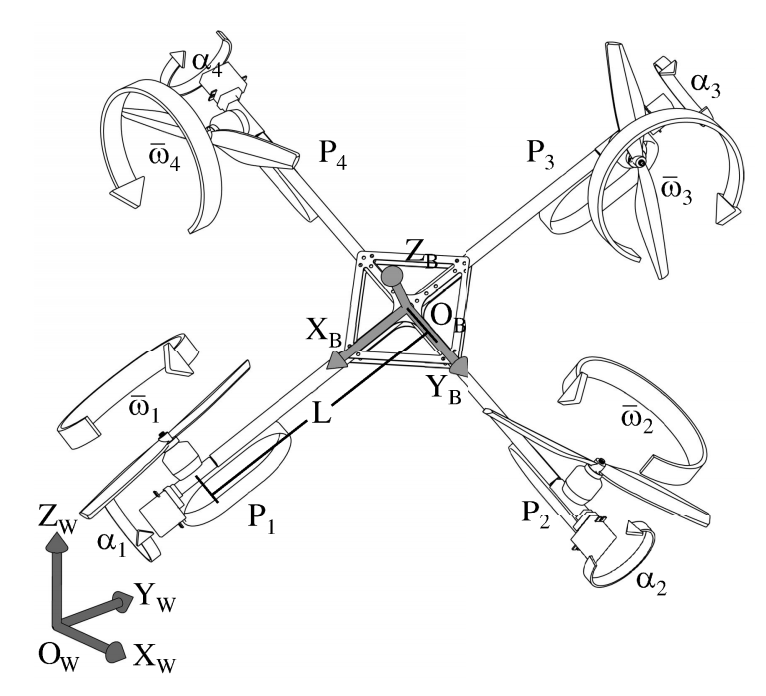
\includegraphics[width=0.65\columnwidth]{ryll_scheme}
	\caption{ -- Общая схема БЛА, расмматриваемого в работе \cite{Ryll01} (рисунок авторов)}
 	\label{fig:ryll_scheme}
\end{figure}
%%%!"!!!!!!!!!!!!!!!!!!!!!!!!!!!!!!!!!!!!

В вектор состояния входят координаты ценра масс аппарата и его ориентация, представленная в матричном виде.
В качестве компонент вектора управляющего воздействия выбраны скорости изменения оборотов двигателей с пропеллерами и скорости поворота двигателей вокруг соответсвующих лучей.
\begin{equation} \label{eq:ryll_ctrl_out}
\begin{aligned}
&\bm{u} = (\dot{\bm \omega}_u,  \dot{\bm \theta}_u)^T,
\\
\bm \omega_u =
(\tilde\omega_1 |\tilde\omega_1|,
\tilde\omega_2 |\tilde\omega_2|&,
\tilde\omega_3 |\tilde\omega_3|,
\tilde\omega_4 |\tilde\omega_4|)^T,
\quad
{\bm \theta}_u = (\theta_1, \theta_2 , \theta_3 , \theta_4 )^T.
\end{aligned}
\end{equation}

Для синтеза контура управления авторы упрощают динамическую модель, принебрегая некоторыми эффектами,
в том числе силой аэродинамического сопротивления, гироскопическими эффектами со стороны корпуса аппарата и роторов с пропеллерами. Преобразованная модель принимает вид
\begin{equation} \label{eq:ryll_dyn}
\begin{aligned}
&\ddot{\bm r}_I = \bm F_g + \frac{1}{m}~^I \bm R_B \bm F(\bm \theta_u) \bm \omega_u,
\\
&\dot {\bm \Omega}_B = \bm J_B \bm T(\bm \theta_u) \bm \omega_u,
\end{aligned}
\end{equation}
где матрицы $\bm F(\bm \theta_u)$ и $\bm T(\bm \theta_u)$ отвечают за текущую геометрию аппарата и с учетом выбранной схемы (рис.\ref{fig:ryll_scheme}) 
\begin{equation} \label{eq:ryl_dyn_matrixes}
\begin{aligned}
&\bm F(\bm \theta) =
\begin{bmatrix}
0&-ks_2&0&ks_4\\
-ks_1&0&ks_3&0\\
kc_1&-kc_2&kc_3&-kc_4
\end{bmatrix},
\\
\phantom{}
\\
&\bm T(\bm \theta) =
\begin{bmatrix}
0&-Lkc_2&0&Lkc_4\\
-Lkc_1&0&Lkc_3&0\\
-Lks_1&Lks_2&-Lks_3&Lks_4
\end{bmatrix}
+
\begin{bmatrix}
0&-bs_2&0&bs_4\\
bs_1&0&-bs_3&0\\
-bc_1&-bc_2&-bc_3&-bc_4
\end{bmatrix}, 
\end{aligned}
\end{equation}
где $c_i = \cos(\theta_i)$, $s_i = \sin(\theta_i)$.
Затем выражения \eqref{eq:ryll_dyn} дифференцируют по времени
\begin{equation} \label{eq:ryll_dyn_dot}
\begin{aligned}
\begin{bmatrix}
&\dddot{\bm r}_I
\\
&\ddot{\bm \Omega}_B
\end{bmatrix}
=
\bm A(\bm \theta_u, \dot {\bm \omega}_u)
\begin{bmatrix}
&\dot{\bm \omega}_u
\\
&\dot{\bm \theta}_u
\end{bmatrix}
+
\bm b(\bm \theta_u, \bm \omega_u, \bm \Omega_B).
\end{aligned}
\end{equation}
Для решения поставленной задачи управления авторы синтезирует регулятор,
\begin{equation} \label{eq:ryll_reg}
\begin{aligned}
\dddot{\bm{r}_d}(t)&=
\dddot{\bm{r}}^0(t) +
\bm{K}_{r1}(\ddot{\bm{r}}^0(t) - \ddot{\bm{r}}(t)) +
\bm{K}_{r2}(\dot{\bm{r}}^0(t) - \dot{\bm{r}}(t)) + 
\bm{K}_{r3}\delta \bm r,
\\
\ddot{\bm{\Omega}_d}(t)&=
\ddot{\bm{\Omega}}^0(t)
+ \bm{K}_{\Omega1}(\dot{\bm{\Omega}}^0(t)-\dot{\bm{\Omega}}(t))
+ \bm{K}_{\Omega2}(\bm{\Omega}^0(t)-\bm{\Omega}(t))
+ \bm{K}_{\Omega3}\delta\bm{R},
\end{aligned}
\end{equation}
сходимость которого обеспечивается выбором матриц коеффициентов $\bm K_{\times}$, которые должны удовлетворять критерию Рауса-Гурвица, а затем обращают динамику и находят вектор $\bm u$, используя псевдообращение Мура-Пенроуза \cite{Barata01}
\begin{equation} \label{eq:ryll_inversed}
\begin{aligned}
\begin{bmatrix}
&\dot{\bm \omega}_u
\\
&\dot{\bm \theta}_u
\end{bmatrix}
=
\bm A^+ \left(
\begin{bmatrix}
&\dddot{\bm r}_I
\\
&\ddot{\bm \Omega}_B
\end{bmatrix}
+
\bm b
\right)
+
(\bm E_8 - \bm A^+ \bm A) \bm \zeta.
\end{aligned}
\end{equation}

Вектор $\bm \zeta$ позволяет использовать две дополнительные степени свободы, возникающих в результате того, что размерность вектора управляющих воздействий превышает размерность вектора состояния, для поддержания ненулевых значений оборотов двигателей, что необходимо для возможности псевдообращения матрицы $\bm A$.

Авторы отмечают, что при реализации обратных связей в контуре управления возможны сложности
с оценкой второй производной текущего положения и ориентации, входящих в регулятор \eqref{eq:ryll_reg},
так как численное дифференцирование сигнала инерциальных датчиков приведет к высокому уровню шума.
Для оценки этих параметров движения предложно воспользоваться выражениями \eqref{eq:ryll_dyn_dot}.
При этом позиция, скорость, ориентация и угловая скорость
измеряется с помощью внешней следящей системы,
также на борту обеспечены измерения оборотов двигателей и углов отклонения сервоприводов.

Для уточнения параметров динамики модели авторы проводят ряд измерений, экспериментально уточняя аэродинамические свойства пропеллеров и переходные процессы в сервоприводах, отвечающих за наклон двигателей.

В работе приводятся численные эксперименты, а после исследователи демонстрируют воплощение алгоритмов управления в прототипе.
В качестве траектории показательного полета выбрана плоская "восьмерка".
Ошибка позиционирования БЛА составила около 5 сантиметров, ориентации -- не более 0,1 радиана.

Основным преимуществом этой работы является детальное рассмотрение управляемой динамики БЛА с поворотными роторами, подробное описание алгоритмов и способов инженерной реализации БЛА такой конструкции.
К недостаткам можно отнести необходимость оценки рывка и углового ускорения в каждый момент времени, а предложенный способ такой оценки, основанный на использовании упрощенной модели \eqref{eq:ryll_dyn_dot} имеет ограничения, связанные с исключением из модели сил аэродинамического сопротивления и гироскопических моментов, что может приводить к значительным ошибкам при некоторых условиях, например, наличии порывов ветра. Другим недостатком является отсутствие реализации строгих ограничений на компоненты вектора управляющих воздействий. Некоторый анализ и дополнения к работе \cite{Ryll01} предложены в исследовании \cite{Stolc01}.

В работе  \cite{Invernizzi01} также рассматривается управляемая динамика квадрокоптера с поворотными роторами. В основе синтеза системы управления лежит ряд геометрических приобразований модели динамики мультироторного робота, для чего пришлось значительно ее упростить.
Для учета ограничений на максимальные углы отклонения поворотных роторов авторы запретили выходить вектору общей тяги аппарата из конусовидной области, параметры которой опредяляются пределами отклонения сервоприводов.
Численные эксперименты показали способность аппарата отслеживать траекторию в виде плоской восьмерки, одновременно меняя свою ориентацию.
При этом углы отклонения сервоприводов не вышли за пределы обозначенных пределов, однако, как сами пояснили авторы, они еще не смогли доказать, что применение такого метода всегда будет гарантировать такой результат.

Еще один пример использования поворотных роторов в конструкции квадрокоптера -- работа \cite{Nemati01}.
Авторы рассматривают аппарат \textit{plus}-конфигурации.
Модель подразумевает возможность симметрично поворачиваться одной паре двигателей.
Авторы применяют метод линеаризаци обратной связи и показывают, что таким образом возможно осуществлять движение и независимо управлять углом тангажа.

Другую техникку для синтеза управления квадрокоптера с поворотными роторами применили в исследовании \cite{Falconi01}.
Замена переменных в модели помогли им численно обратить динамику БЛА и получить выражения для углов отклонения двигателей и оборотов каждого из них, чтобы выход системы соостветсвовад выходу ПД регулятора, который обеспечивает сходимость положения и ориентации БЛА к целевым.
Вычислительные эксперименты показали работоспособность предложенного алгоритма.

Скользящий режим для синтеза контура управления БЛА с поворотными роторами применяется в \cite{Yih01}. 
Численные эксперименты подтвердили способность аппарата перемещаться в точку при неизменной ориентации корпуса.

Исследование маневренных возможностей квадрокоптеров с поворотными роторами с большими пределами отклонений сервоприводов проведено в работе \cite{Oosedo01}.
Показана возможность полета с углами тангажа и рысканья окло 90 градусов.
Проведены летные испытания.

Вычислительно простой способ управления БЛА с поворотными роторами разработан в \cite{Alkamachi01}. Рассмотрена нестандартная схема, где каждый из двигателей может вращаться вокруг луча,
параллельного поперечной оси корпуса аппарата.
Для управления позицией и ориентацией использовались ПИД-регуляторы.
Все роторы наклоняются синхронно.
Контур управления показал хорошую производительность в условиях внешних возмущений, шума измерений и неопределенности в параметрах динамики БЛА.


	
\chapter{Управляемая динамика квадрокоптера с поворотными роторами}
\label{chapter_dyn}

\section{Основные элементы конструкции квадрокоптера с поворотными роторами}

Основным элементом конструкции БЛА является корпус, из которого выходят лучи с закрепленными на концах двигателями с пропеллерами. Лучи расположены симметрично относительно корпуса аппарата и реализуют так называемую Х-схему. Смежные пропеллеры имеют противоположное направление вращения; первый и третий – пропеллеры левого вращения, а второй и четвертый – правого. Каждый из роторов может поворачиваться посредством сервопривода вокруг продольной оси луча, на котором он закреплен. Для построения математической модели динамики БЛА условимся, что он сконструирован таким образом, что
\begin{itemize}
	\item главные центральные оси инерции аппарата и каждого из роторов совпадают с осями симметрии; 
	\item корпус БЛА и каждый из четырех роторов являются твердыми телами; 
	\item под ротором будем понимать вращающуюся часть двигателя и жестко связанный с ним пропеллер; 
	\item крепление роторов к корпусу БЛА происходит в точке, совпадающей с центрами масс роторов, помимо роторов спрпелеерами в системе отсутствуют подвижные части;
	\item центры масс роторов лежат на окружности радиуса $L$, центр окружности совпадает с центром масс корпуса аппарата.
\end{itemize}
Общий вид аппарата представлен рисунке \ref{fig:tiltrotor_scheme}.

\begin{figure}[h]
	\centering
	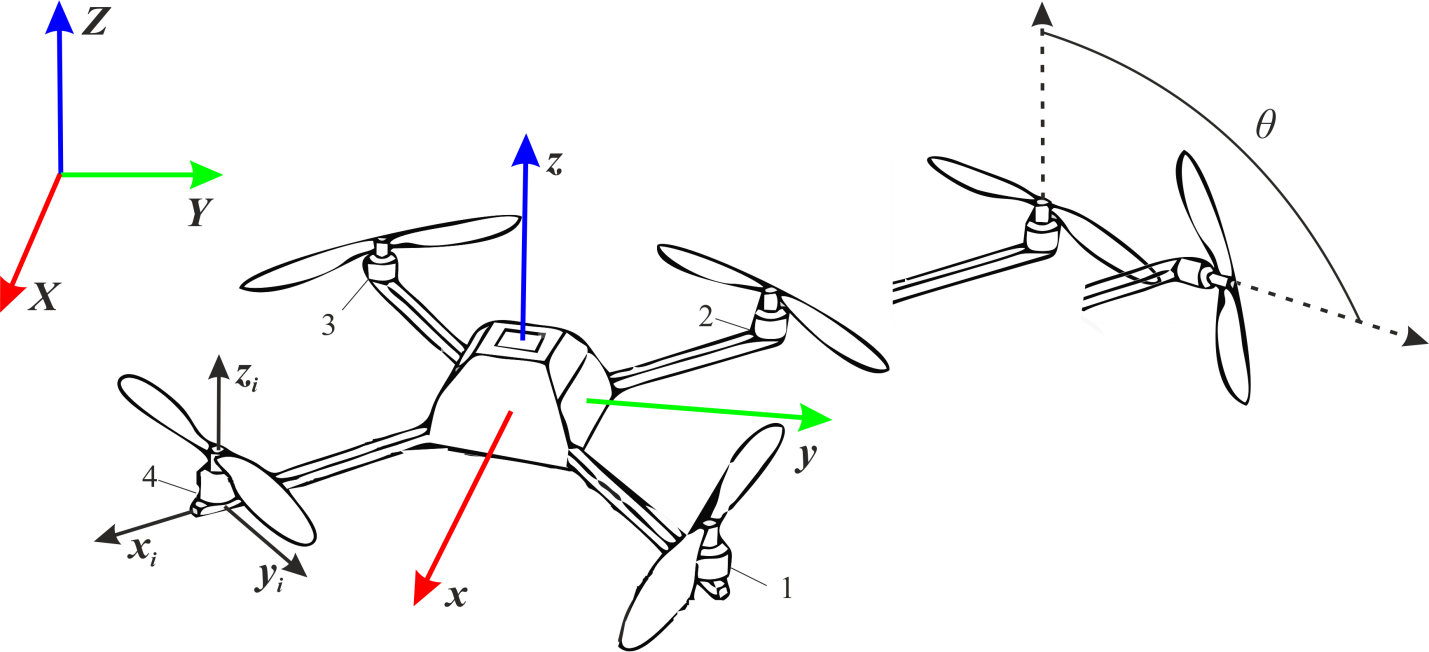
\includegraphics[scale=0.9]{tiltrotor_scheme}
	\caption{ -- Общая схема квадрокоптера с поворотными роторами}
	\label{fig:tiltrotor_scheme}
\end{figure}

\section{Постановка задачи управления}
\label{section_ctrl_task}
	
Считая заданной требуемую траекторию БЛА в координатном пространстве, положим целью управления обеспечение наперёд заданной траектории центра масс аппарата, а также требуемой ориентации. Такая постановка позволяет формализовать следующие задачи:
\begin{itemize}
\item приведение центра масс БЛА в некоторое наперёд заданное статичное положение;
\item стабилизация ориентации БЛА относительно некоторого наперёд заданного положения;
\item перемещение центра масс БЛА вдоль некоторой наперёд заданной (дискретным набором точек или как непрерывная функция координат от времени) траектории;
\item слежение за объектом, перемещающимся произвольным образом;
\item наведение камеры, установленной на БЛА на неподвижный или перемещающийся объект (то есть съёмка неподвижного объекта с разных ракурсов или слежение камерой за подвижным объектом).
\end{itemize}

Решение последней задачи в явном виде использует степени свободы, связанные с увеличением размерности вектора управляющих параметров. Стоит отметить, что квадрокоптер со стандартной конструкцией произвольный манёвр наведения камеры в точку с одновременным изменением высоты выполнить не способен.

\section{Математическая модель динамики БЛА}

Движение аппарата рассматривается относительно неподвижной инерциальной системы отсчета $I$, связанной с Землей (вращением Земли на характерных временах автономного полёта БЛА рассматриваемого класса принято пренебрегать).
Направление осей выбрано по схеме «Восток, Север, Верх» (ENU) -- ось \textbf{$X_I$} направлена на восток, ось \textbf{$Y_I$} -- на север, а ось \textbf{$Z_I$} -- от центра Земли.

Индексом $B$ обозначим жестко связанную с корпусом аппарата систему координат с началом в центре масс и осями, совпадающими с главными центральными осями инерции корпуса БЛА.
Для промежуточных выкладок нами будет использована ещё одна жестко связанная с корпусом система координат $B'$, полученная из $B$ поворотом вокруг оси $Z_B$ таким образом, что ось $X_B'$ направлена вдоль луча, несущего первый ротор согласно схеме \ref{fig:tiltrotor_scheme}.

Индексами $R_i$ будем обозначать системы координат, жестко связанные с роторами и совпадающие с их главными центральными осями инерции.

При записи векторов будем отмечать верхним индексом систему координат, в которой записано разложение вектора. Повороты систем координат друг относительно друга будем описывать кватернионами. Будем говорить, что кватернион $q_{IB}$ задаёт ориентацию системы координат $B$ относительно $I$ в том смысле, что разложения некоторого вектора $\bm{r}$ в этих двух базисах связаны соотношением
\begin{equation} \label{eq:m_quat}
\bm{r}^I = q_{IB} \circ \bm{r}^B \circ \tilde{q}_{IB}.
\end{equation}

Положение БЛА в пространстве определяется радиус-вектором его центра масс $\bm{r}^I$ и кватернионом ориентации $q_{IB}$. Скорость центра масс аппарата равна
\begin{equation} \label{eq:m_vel}
\bm{v}^I = \dot{\bm{r}^I}.
\end{equation}
Изменение кватерниона ориентации аппарата определяется уравнением Пуассона
\begin{equation} \label{eq:m_puasson}
\dot{q}_{IB} = \frac{1}{2} {q}_{IB} \circ \bm{\Omega}^B,
\end{equation}
где $\bm{\Omega}_B$ – угловая скорость корпуса БЛА в проекции на собственные оси.

Движение центра масс БЛА определяется уравнением
\begin{equation} \label{eq:m_traslational_motion}
M \ddot{\bm{r}} = M \bm{g}^I - \frac{1}{2} \rho C S_{\perp} |\bm{v}^I| \bm{v}^I + \sum_{i=1}^{4}{ { (-1)^{i+1} k \tilde \omega_i |\tilde \omega_i| \bm{e}^I_{z_i}}},
\end{equation}
где три члена в правой части соответствуют силе тяжести, силе аэродинамического сопротивления и создаваемой пропеллерами тяге, $M = m + \sum_{i=1}^{4}{m_i}$ – общая масса корпуса, $m_i$ – масса $i$-го ротора с пропеллером, $\bm g$ – ускорение свободного падения, $S_{\perp}$ – площадь миделева сечения корпуса аппарата, $C$ – аэродинамический коэффициент сопротивления воздуха, $\bm{e}^I_{z_i}$ – единичный вектор вдоль оси симметрии i-го ротора, $k$ – аэродинамический коэффициент, определяемый экспериментально; $\tilde \omega_i$ – скорость вращения i-го пропеллера.

Для описания вращательного движения воспользуемся динамическими уравнениями Эйлера
\begin{equation} \label{eq:m_rotational_motion}
\bm{\tau}^{B} =
\bm{J}_B\dot{\bm{\Omega}}^B + \bm{\Omega}^B \times \bm{J}_B{\bm{\Omega}^B},
\end{equation}
где $\bm{J}_B$ — тензор инерции корпуса в главных осях корпуса; $\bm{\tau}^{B}$ —
главный момент сил, действующий на корпус.

Главный момент сил складывается из моментов сил, действующих на корпус аппарата со стороны поворотных роторов с пропеллерами и внешних моментов:
\begin{equation} \label{eq:m_general_torq}
\bm{\tau}^{B} =
-\sum_{i=1}^{4} {\bm{\tau}^{B}_i} +
\sum_{i=1}^{4} {\bm{r}^B_i \times (-1)^{i+1} k \tilde \omega_i |\tilde \omega_i| \bm{e}^{B}_{z_i},}
\end{equation}
где $\bm{\tau}^{B}_i$ — моменты сил, действующие на роторы со стороны аппарата, $\bm{r}^B_i$ -- радиус вектор, проведенный из центра масс квадрокоптера $i$-тому к ротору. Вычислим угловую скорость $i$-го ротора в проекциях на оси $R_i$:
\begin{equation} \label{eq:m_prop_ang_vel}
\bm{\omega}^{R_i}_i =
q_{{R_i} B} \circ (\bm{\Omega}^B + \dot {\theta}_i \bm e^B_{r_i}) \circ \tilde {q}_{{R_i}B} +
\tilde \omega_i \bm{e}^{R_i}_{z_i},
\end{equation}
где $\bm e^B_{r_i}$ -- орт вектора $\bm{r}^B_i$, ${\theta}_i$ -- угол поворота $i$-того ротора. Запишем динамические уравнения Эйлера для роторов:
\begin{equation} \label{eq:m_rotors_dyn}
\bm{\tau}^{{R_i}}_i + \bm{\varsigma}^{{R_i}}_{i} = 
\bm{J}_{R_i}\dot{\bm{\omega}}^{R_i}_i + \bm{\omega}^{R_i}_i \times \bm{J}_{R_i}{\bm{\omega}^{R_i}_i},
\end{equation}
где $\bm{J}_{R_i}$ -- тензор инерции $i$-того ротора с пропеллером, записанный в собственных главных осях, $\bm{\varsigma}^{{R_i}}_{i}$ -- внешний момент силы, для которго запишем:
\begin{equation} \label{eq:m_ext_torq}
\begin{aligned}
&\bm{\varsigma}^{{R_i}}_{i} = -b \tilde \omega_i |\tilde \omega_i| \bm e^{R_i}_{r_i}\\
&\bm{\varsigma}^{B}_{i} = q_{ B {R_i}} \circ \bm{\varsigma}^{{R_i}}_{i} \circ \tilde q_{ B {R_i}}.
\end{aligned}
\end{equation}
Здесь $b$ -- аэродинамический коэффициент, определяемый экспериментально.

Окончательно уравнения вращательной динамики аппарата принимают вид:
\begin{equation} \label{eq:m_final_rotational_motion}
\begin{aligned}
\bm{J}_B\dot{\bm{\Omega}}^B + \bm{\Omega}^B \times \bm{J}_B{\bm{\Omega}^B} =
&\sum_{i=1}^{4} {\bm{r}^B_i \times
	(-1)^{i+1} k \tilde \omega_i |\tilde \omega_i| \bm{e}^B_{z_i}} + \\ +
\sum_{i=1}^{4} {\bm{\varsigma}^{{R_i}}_{i}} +
&\sum_{i=1}^{4} q_{ B {R_i}} \circ (\bm{J}_{R_i}\dot{\bm{\omega}}^{R_i}_i + \bm{\omega}^{R_i}_i \times \bm{J}_{R_i}{\bm{\omega}^{R_i}_i}) \circ \tilde q_{ B {R_i}}
\end{aligned}
\end{equation}
Уравнения (\ref{eq:m_vel}), (\ref{eq:m_puasson}), (\ref{eq:m_traslational_motion}) и (\ref{eq:m_final_rotational_motion}) составляют замкнутую систему, позволяющую моделировать динамику полета квадрокоптера с поворотными роторами.

\section{Синтез регулятора}

Пусть задана требуемая траектория центра масс аппарата $\bm r^0(t)$, а также требуемая ориентация $q^0(t)$. Обозначим  $\delta \bm r(t) = \bm r^0(t) - \bm r(t)$ и $\delta q(t) = q^0(t) \circ \tilde q(t)$, где $\delta \bm r$ и $\delta q$ определяют расхождение требуемой и текущей траектории БЛА в координатном пространстве, а $q = q_{IB}$.  В качестве переменных управления выберем скорости вращения пропеллеров ${\tilde \omega}_i$ и углы поворота роторов ${\theta}_i$:
\begin{equation} \label{eq:m_ctrl_out}
\begin{aligned}
	&\bm{u} = (\bm \omega_u, \bm \theta_u)^T,
	\\
	\bm \omega_u =
	(\tilde\omega_1 |\tilde\omega_1|,
	\tilde\omega_2 |\tilde\omega_2|&,
	\tilde\omega_3 |\tilde\omega_3|,
	\tilde\omega_4 |\tilde\omega_4|)^T,
	\quad
	\bm \theta_u = (\theta_1, \theta_2 , \theta_3 , \theta_4 )^T.
\end{aligned}
\end{equation}
Регуляторы, обеспечивающие необходимое управление по положению и ориентации могут быть построены, как
\begin{equation} \label{eq:m_reg}
\begin{aligned}
	\ddot{\bm{r}_d}(t)&=
	\ddot{\bm{r}}^0(t)+\bm{K}_{r1}(\dot{\bm{r}}^0(t) - \dot{\bm{r}}(t))+\bm{K}_{r2}\delta \bm r,\\
	\dot{\bm{\Omega}}_d(t)&=
	\dot{\bm{\Omega}}^0(t)+\bm{K}_{\Omega1}(\bm{\Omega}^0(t)-\bm{\Omega}(t))+\bm{K}_{\Omega2}\delta\bm{q},
\end{aligned}
\end{equation}
где $\delta \bm q$ -- векторная часть кватерниона $\delta q$,
$\ddot{\bm{r}}^0$, $\dot{\bm{r}}^0$, $\ddot{\bm{\Omega}}^0$, $\dot{\bm{\Omega}}^0$ -- целевое ускорение, скорость, угловое ускорение и угловая скорость соответственно,
$\bm K_{r1}$, $\bm K_{r2}$, $\bm K_{\Omega1}$, $\bm K_{\Omega2}$ -- диагональные матрицы коэффициентов, выбор которых согласно критерию Рауса-Гурвица гарантирует сходимость траектории аппарата к требуемой. Таким образом, для построения
контура управления, необходимо связать выход из регулятора с управляющими
параметрами, учесть присутствующие в системе ограничения на реализацию
управляющих воздействий, а также реализовать обратные связи.

\section{Обращение динамики модели}
\label{section_dyn_inverse}

Реализация контура управления с регуляторами (\ref{eq:m_reg}) требует обращения динамики системы, то есть определения значений всех управляющих параметров (\ref{eq:m_ctrl_out}) по выходу из регулятора (\ref{eq:m_reg}).
Для достижения этой цели преобразуем уравнения модели (\ref{eq:m_vel}), (\ref{eq:m_puasson}), (\ref{eq:m_traslational_motion}), (\ref{eq:m_final_rotational_motion}).
Сначала перепишем их в проекциях на оси системы координат $B'$, а затем
преобразуем таким образом, чтобы в правой части получившихся выражений остались все члены, в которые явно входят управляющие параметры (\ref{eq:m_ctrl_out}), а все остальные члены перенесём в левую часть. Таким образом, получим систему уравнений
\begin{equation} \label{eq:m_dyn}
\begin{aligned}
&\bm F(\ddot{\bm r}_d, \dot{\bm r}, q) = k F_{thr} (\bm \theta_u) \bm \omega_u,\\
&\bm T(\dot{\bm \Omega}_d, \bm\Omega) = \Big(
kLT_{thr}(\bm\theta_u) - bT_{aero}(\bm\theta_u)
\Big)
\bm \omega_u.
\end{aligned}
\end{equation}
Матрицы в правой части уравнений принимают вид (\ref{eq:m_dyn}):
\begin{equation} \label{eq:m_dyn_matrixes}
\begin{aligned}
&F_{thr} =
\begin{bmatrix}
0&-s_2&0&s_4\\
-s_1&0&s_3&0\\
c_1&-c_2&c_3&-c_4
\end{bmatrix},
\\
\phantom{}
\\
&T_{thr} =
\begin{bmatrix}
0&-c_2&0&c_4\\
-c_1&0&c_3&0\\
-s_1&s_2&-s_3&s_4
\end{bmatrix},
\\
\phantom{}
\\
&T_{aero} =
\begin{bmatrix}
0&s_2&0&-s_4\\
-s_1&0&s_3&0\\
c_1&c_2&c_3&c_4
\end{bmatrix},
\end{aligned}
\end{equation}
где $c_i = \cos(\theta_i)$, $s_i = \sin(\theta_i)$.

Система (\ref{eq:m_dyn}) недоопределена и нелинейна относительно компонент $\bm \theta_u$, что значительно затрудняет ее аналитическое решение. Доопределим систему, используя выражения для распределения вертикальных составляющих сил и моментов между парами двигателей, расположенных на параллельных лучах
\begin{equation} \label{eq:m_dyn_balance_1}
\begin{aligned}
&k \tilde\omega_1 |\tilde\omega_1| c_1 + k \tilde\omega_3 |\tilde\omega_3| c_3 =
\frac{1}{2} \bm F_z + \varepsilon_F,
\\
&\tilde\omega_1 |\tilde\omega_1| (bc_1 - kLs_1)
+ \tilde\omega_3 |\tilde\omega_3| (bc_3 - kLs_3) =
\frac{1}{2} \bm T_z + \varepsilon_T,
\end{aligned}
\end{equation}


\begin{equation} \label{eq:m_dyn_balance_2}
\begin{aligned}
&k \tilde\omega_2 |\tilde\omega_2| c_2 + k \tilde\omega_4 |\tilde\omega_4| c_4 =
-\frac{1}{2} \bm F_z + \varepsilon_F,
\\
&\tilde\omega_2 |\tilde\omega_2| (bc_2 + kLs_2)
+ \tilde\omega_4 |\tilde\omega_4| (bc_4 + kLs_4) =
\frac{1}{2} \bm T_z - \varepsilon_T,
\end{aligned}
\end{equation}
где $\varepsilon_F$ и $\varepsilon_F$ -- балансировочные параметры.

Полученная система уравнений (\ref{eq:m_dyn}), (\ref{eq:m_dyn_balance_1}) имеет аналитическое решение:
\begin{equation} \label{eq:m_dyn_resolve}
\begin{aligned}
&\tilde\omega_i |\tilde\omega_i| =
\frac{(-1)^{i+1}}{2kL}\sqrt{
A^2_i + 
B^2_i},
\\
\phantom{}
\\
&\theta_i = 
2 \text{arctg} \Bigg[(-1)^{i+1}	
\frac{A_i -
\sqrt{A^2_i +
B^2_i
}}
{B_i}
\Bigg],
\end{aligned}
\end{equation}
где $A_i = A_i(\bm F, \bm T, \varepsilon_F, \varepsilon_T)$
и
$B_i = B_i(\bm F, \bm T, \varepsilon_F, \varepsilon_T)$
-- скалярные функции, куда линейно входят компоненты левой части уравнений динамики \eqref{eq:m_dyn}
$\bm F(\ddot{\bm r}_d, \dot{\bm r}, q)$
и
$\bm T(\dot{\bm \Omega}_d, \bm\Omega)$.
Выражения для $A_i$ и $B_i$ приведены в Приложении А
(\ref{eq:app_solve_AB_begin}-\ref{eq:app_solve_AB_end}).
Таким образом, полученное решение связывает выход регулятора с управляющими параметрами при наличии обратной связи, а именно известных текущих координате $\bm r^I$, скорости $\bm v^I$, ориентации $q_{IB}$ и угловой скорости $\bm \Omega^B$.

\section{Динамика исполнительных органов системы управления}

Полученные в предыдущем разделе выражения для аналитического обращения динамики БЛА \eqref{eq:m_dyn_resolve} позволяют найти целевые значения оборотов двигателей и углов отклонения сервоприводов, оценив текущее состояние и выбрав траекторию движения.
Однако, динамика исполнительных органов системы управления может накладывать собственные ограничения на возможность обеспечить соответствие между реальными и целевыми значениями компонент вектора управляющих воздействий.

Как показывает практика \cite{Ryll01, Mellinger01}, параметры современных двигателей, используемых при проектировании малых беспилотных летательных аппаратов, позволяют развить требуемые контуром управления обороты достаточно быстро, чтобы не учитывать эту задержку при синтезе контура управления.
При этом небольшие сервоприводы, которые обычно используют при конструировании БЛА небольшого размера, обычно имеют весьма ограниченную угловую скорость выходного вала при внушительном максимальном крутящем моменте \cite{RobotShop}. Чтобы учесть эти особенности, не вдаваясь в подробности внутреннего устройства приводных механизмов, дополним модель
(\ref{eq:m_vel}),
(\ref{eq:m_puasson}),
(\ref{eq:m_traslational_motion}), (\ref{eq:m_final_rotational_motion})
выражениями для динамики сервоприводов, которые запишем в виде
\begin{equation} \label{eq:m_servo_target}
\dot{\bm{\theta}} = \bm{K}_{\theta} (\bm{\theta}_{u} - \bm{\theta}),
\end{equation}
где 
$\bm{K}_{\theta}$ -- диагональная матрица положительных коэффициентов, характеризующая параметры исполнительных механизмов.
Такая формулировка \eqref{eq:m_servo_target} закона движения выходного вала сервопривода позволяет обеспечить непрерывный характер функции изменения угла его поворота от времени при моделировании управляемой динамики БЛА и ограничить максимальную скорость поворота значением
\begin{equation} \label{eq:m_servo_dot_max}
\dot{\bm{\theta}}_{max} =
2 \bm{K}_{\theta}
\bm{\theta}_{max},
\end{equation}
где  $\bm{\theta}_{max}$ -- вектор максимальных значений отклонений сервоприводов.

Так как динамика исполнительных органов системы управления БЛА не позволяет обеспечить соответсвие между найдеными на основе обращения динамики углами отклонения сервоприводов и их реальными значениями, необходимо разработать решение, учитывающее эту динамику, с помощью которого можно решить поставленную задачу управления.
В качестве такого решения предлагается использовать второй регулятор, который будет стабилизировать ориентацию корпуса аппарата и его высоту, когда как ошибка позиционирования в горизонтальной плоскости будет зависеть от способности сервоприводов отслеживать целевые углы.

Пусть известны текущие углы ориентации $\tilde {\bm {\theta}}$, которые могут отличаются от целевых $\bm \theta_u$.
Тогда составим вектор управляющих воздействий только из значений оборотов двигателей
\begin{equation} \label{eq:m_cut_ctrl_out}
\begin{aligned}
&\bm{u} = (\bm \omega_u)^T,
\\
\bm \omega_u =
(\tilde\omega_1 |\tilde\omega_1|&,
\tilde\omega_2 |\tilde\omega_2|,
\tilde\omega_3 |\tilde\omega_3|,
\tilde\omega_4 |\tilde\omega_4|)^T,
\end{aligned}
\end{equation}
Исключим из уравнений модели \eqref{eq:m_dyn} выражения, отвечающие за движение в горизонтальной плоскости, с учетом известных в текущий момент углов отклонения сервоприводов запишем
\begin{equation} \label{eq:m_cut_dyn}
\begin{aligned}
&\bm F_z(\ddot{\bm r}_d, \dot{\bm r}, q) =
k {F_z}_{thr} (\tilde{\bm \theta}) \bm \omega_u,\\
&\bm T(\dot{\bm \Omega}_d, \bm\Omega) =
\Big(
kLT_{thr}(\tilde{\bm \theta}) - bT_{aero}(\tilde{\bm \theta})
\Big)
\bm \omega_u.
\end{aligned}
\end{equation}
Тогда, если обозначить
\begin{equation}
\bm Y = 
\begin{bmatrix}
&\bm F_z \\
&\bm T \\
\end{bmatrix}
\end{equation}
\begin{equation}
\bm A = 
\begin{bmatrix}
&k {F_z}_{thr} \\
&kLT_{thr} - bT_{aero}
\end{bmatrix}
\end{equation}
вектор управляющих воздействий может быть вычислен, как
\begin{equation}
\bm \omega_u = 
\bm A^{-1} \bm Y
\end{equation}
Таким образом, зная текущие углы отклонения сервоприводов можно найти обороты двигателей, которые обеспечат некоторые из целевых параметров движения, а именно ориентацию и высоту. Отсутствие полного соответствия между целевыми $\bm \theta_u$ и текущими $\tilde {\bm \theta}$ углами приведет к возникновению ошибки позиционирования в горизонтальной плоскости. Однако, вычислительные эксперименты, представленные в главе \ref{experiments_chapter} показывают, что параметры сервоприводов, используемых при проектировании небольших БЛА позволяют добиться достаточной точности для решения практических задач, например для наблюдения за подвижным объектом с помощью неподвижной бортовой камеры.

\section{Введение ограничений на компоненты вектора управляющих воздействий}
\label{section:limits}

Проанализируем полученные выражения для компонет вектора управляющих воздействий (\ref{eq:m_dyn_resolve}) и введем ограничения на максимальную скорость вращения роторов и на углы отклонения сервоприводов.

Заметим, что при $B_i = 0$ соответсвующий угол отклонения $\theta_i$ не определен. Найдем область допустимых значений функции $\theta_i(A_i, B_i)$.
Функция определена, когда определена функция под арктангенсом
\begin{equation}
f_{\theta}(A_i, B_i) = \frac{A_i-\sqrt{A^2_i +  B^2_i}}{B_i}.
\end{equation}
Предел функции $f_{\theta}(A_i, B_i)$ при $B_i \to 0$.
\begin{equation}
\lim_{B_i \to 0} f_{\theta}(A_i, B_i) =
\frac{{A_i} - |A_i|}{B_i} + 
\frac{B_i}{2A_i}
\end{equation}
Значение предела, а следовательно и угол $\theta_i(A_i, B_i)$, определено всюду, кроме луча (см. рис. \ref{fig:f_th})
\begin{equation} \label{m_theta_exists}
\begin{aligned}
&A_i \leq 0, \\
&B_i = 0.
\end{aligned}
\end{equation}
\begin{figure}[h!]
	\centering
	\includegraphics[width=12cm,clip]{DAB.eps}
	\caption{ -- Поверхность $f_{\theta}(A_i, B_i)$}
	\label{fig:f_th}
\end{figure}
Положим 
\begin{equation} \label{eq:m_limits_init}
\begin{aligned}
&0< (-1)^{i+1} \tilde \omega_i |\tilde\omega_i| < \tilde \omega_{max}^2,
\\
&|\theta_i| < \theta_{max} < \pi,
\end{aligned}
\end{equation}
где $\omega_{max}$ и $\theta_{max}$ -- максимальные возможные обороты пропеллеров и углы отклонения сервоприводов.
Используя уравнения обращенной динамики (\ref{eq:m_dyn_resolve}), можно переписать ограничения (\ref{eq:m_limits_init}) в виде
\begin{equation} \label{eq:m_limits_AB}
\begin{aligned}
&0 <
\sqrt{A^2_i +  B^2_i}
< 2 k^2 L\omega_{max}^2,
\\
&\Bigg|\frac{A_i-\sqrt{A^2_i +  B^2_i}}{B_i}\Bigg| < 
\text{tg}\frac{\theta_{max}}{2}.
\end{aligned}
\end{equation}
Найдем область в пространстве $(A_i, B_i)$, в которой будут выполнены данные ограничения. Для этого сначала перейдем в полярные координаты
\begin{equation} \label{eq:m_polar}
\begin{aligned}
&A_i = \rho_i \cos(\varphi_i),
\\
&B_i = \rho_i \sin(\varphi_i).
\end{aligned}
\end{equation}
Тогда выражения (\ref{eq:m_limits_AB}) примут вид
\begin{equation} \label{eq:m_limits_polar_rho}
0 < \rho < 
2 k^2 L\omega_{max}^2
= \rho_{max},
\end{equation}
\begin{equation} \label{eq:m_limits_polar_phi}
\Bigg| \frac{\cos(\varphi_i)-1}{\sin(\varphi_i)} \Bigg| < 
tg\frac{\theta_{max}}{2}.
\end{equation}
Функция (рис. \ref{fig:f_phi})
$$f_{\varphi}(\varphi) = \frac{\cos(\varphi_i)-1}{\sin(\varphi_i)}$$
является монотонной и непрерывной на интервалах 
$(-{\pi}, 0)$
и
$( 0, \pi)$
и имеет предел
$$\lim_{\varphi_i \to 0}
f_{\varphi}(\rho_i, \varphi_i) = 0,$$
значит, система неравенств
\eqref{eq:m_limits_polar_phi}
всегда имеет решение относительно $\varphi_i$ на заданном интервале.
\begin{figure}[h!]
	\centering
	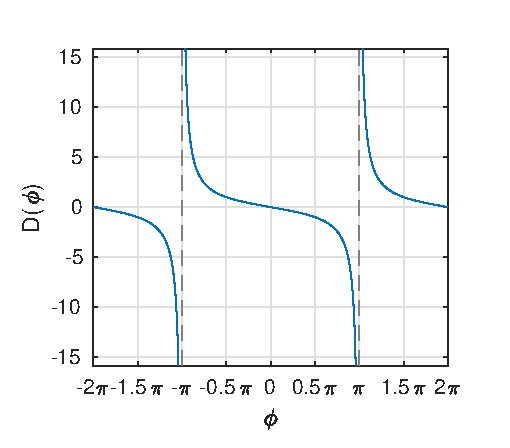
\includegraphics[width=10cm,clip]{Dphi.eps}
	\caption{ -- График $f_{\varphi}(\varphi)$}
	\label{fig:f_phi}
\end{figure}
Разрешив неравенства \eqref{eq:m_limits_polar_phi} и вернувшись к исходной системе ($A_i, B_i$), запишем
\begin{equation} \label{eq:m_limits_new_1}
\sqrt{A^2_i +  B^2_i} <
\rho_{max}
\end{equation}
\begin{equation} \label{eq:m_limits_new_2}
|B_i| < A_i \text{tg} \theta_{max}
\end{equation}

Условия \eqref{eq:m_limits_new_1}, \eqref{eq:m_limits_new_2} формируют область $\Omega_{A_iB_i}$ на плоскости $A_iB_i$, в которой выполняются необходимые ограничения на выходы управления. Область состоит из внутренних точек сектора круга радиуса $\rho_{max}$ и центральным углом $2\theta_{max}$ (рис. \ref{fig:lim_circle}).
Данная область эквивалентна некоторой области $\Omega_{\bm{y}}$ в пространстве вектора  $\bm{y} \in \mathcal{R}^6$, $\bm{y} = (\bm{F}, \bm{T})^T$, из которой можно выделить линейно-ограниченную подобласть $\Omega^*_{\bm{y}}$.
Из выражения \eqref{eq:m_limits_new_1} следует, что
\begin{equation} \label{eq:rho_limits_lin}
\frac{\mid A_i \mid + \mid B_i \mid} {\sqrt2}
< \rho_i^{max}.
\end{equation}

\begin{figure}[h!]
	\centering
	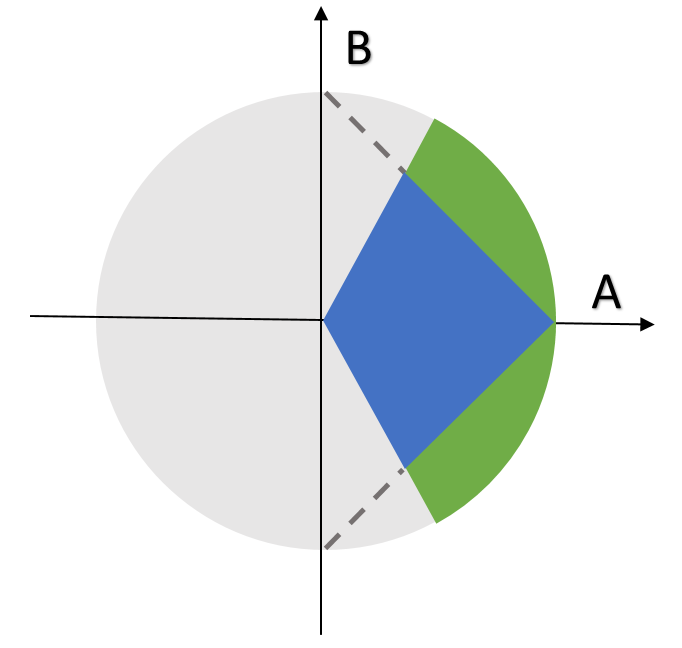
\includegraphics[width=10cm,clip]{circle.png}
	\caption{ -- Иллюстрация области $\Omega_{A_iB_i}$ и выделение из нее линейно-ограниченной подобласти}
	\label{fig:lim_circle}
\end{figure}

Чтобы гарантировать, что ограничения на выходы управления \eqref{eq:m_limits_init} будут выполняться, нужно ограничить выходы регулятора
\eqref{eq:m_reg}
так, чтобы вектор
$\bm y$
принадлежал области
$\Omega_{\bm{y}}$.
Однако, работать с ограничениями в таком виде на практике не всегда удобно. Выделив прямоугольную область $\Psi_{\bm y} \in \Omega^*_{\bm y}$, можно независимо определить ограничения на каждый из компонент вектора $\bm y$:
\begin{equation} \label{rect_in}
y_k^{min} < y_k < y_k^{max},
\quad k = 1 .. 6.
\end{equation}

Для этого выберем центр прямоугольной области
$\bm y^C$
и единичный направляющий вектор ее диагонали
$\bm d$
и найдем значения балансировочных параметров
$\varepsilon_F, \varepsilon_T$,
при которых все точки n-мерного прямоугольника
$\Psi_{\bm y}$
удовлетворяют ограничениям \eqref{eq:m_limits_new_2}, \eqref{eq:rho_limits_lin}, а длина его диагонали $2\gamma$ максимальна (рис. \ref{fig:reqct_finding}).
\begin{figure}[h!]
	\centering
	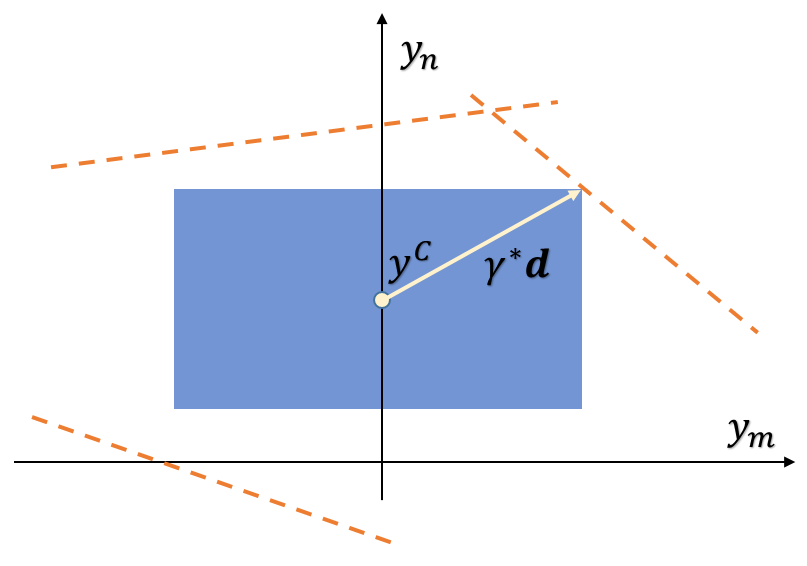
\includegraphics[width=10cm]{rect.png}
	\caption{ -- Поиск прямоугольной области $\Psi_{\boldsymbol{y}}$}
	\label{fig:reqct_finding}
\end{figure}
За центр прямоугольника выберем точку, соответствующую неподвижному зависанию аппарата. 
\begin{equation} \label{center}
\bm y^C = (0, 0, Mg, 0, 0, 0)^T.
\end{equation}
От компонент вектора $\bm d$ будут зависеть абсолютные значения пределов соответствующих компонент выхода регулятора, их выбор может быть обусловлен необходимостью повысить предел насыщения регулятора по некоторым направлениям за счет других. 

Если все вершины прямоугольной области удовлетворяют набору линейных ограничений, то все его внутренние точки также удовлетворяют этим ограничениям. Тогда, достаточно проверить конечное количество точек области $\Psi_{\bm y}$ на принадлежность к области $\Omega^*_{\bm y}$, чтобы убедиться, что ограничения выполняются в каждой точке области $\Psi_{\bm y}$. Это позволяет применить численные методы к поиску значений параметров $\epsilon_F, \epsilon_T$ и максимальной длины диагонали прямоугольника $2\gamma^*$. В итоге ограничения для компонент вектора  при котором выполняются искомые ограничения \eqref{eq:m_limits_init} могут быть записаны в виде

\begin{equation} \label{eq:lims_final}
y^C_k - \gamma^* d_k < y_k < y^C_k + \gamma^* d_k, \quad k = 1 .. 6.
\end{equation}

\section{Экстренное управление при отказе двух смежных двигателей}
\label{section_em_ctrl}

Как было показано в этой главе, расширение размерности вектора управляющего воздействия квадрокоптера позволяет повысить маневренные характеристики аппарата и помогает добиться независимого управления по всем 6-ти степеням свободы.
Однако, при возникникновении нештатной ситуации способность изменять вектор тяги каждого из двигателей может спасти аппарат от неконтролируемого падения.
Хотелось бы отметить, что экстренное управление БЛА является немаловажной частью исследований их управляемой динамики, и данной теме посвящено немало работ \cite{Morozov01, Lippiello01, Mueller01}. В последних из них авторам удалось добиться возможности продолжения миссии квадрокоптера стандартной конструкции с одним вышедшим из строя двигателем на высокой скорости \cite{Sun01} и показать, что успешная посадка аппарата возможна даже при наличии всего двух работающих двигателей, расположенных на противолежащих лучах аппарата \cite{Gomes01}. Подобные исследования проводились также для квадрокоптеров с поворотными роторами, где дополнительные исполнительные органы системы управления, а именно сервоприводы, изменяющие направления тяги оставшихся двигателей, способны частично компенсировать потерю управляемости БЛА вследствие потери одного двигателя \cite{Nemati02}.
Среди нерассмотренных сценариев остается потеря двух смежных двигателей, что вполне может произойти, например, при лобовом столкновении с препятствием, таким как стена здания. Ниже будет рассмотрено движение квадрокоптера с поворотными роторами без двух смежных двигателей.
Без потери общности можно выбрать, например, двигатели, расположенные сзади (второй и третий, рис \ref{fig:tiltrotor_scheme}). Тогда, вектор управляющих воздействий \eqref{eq:m_ctrl_out} примет вид
\begin{equation} \label{eq:em_ctrl_out}
\begin{aligned}
&\bm{u'} = (\bm \omega_u', \bm \theta_u')^T,
\\
\bm \omega_u' =
(\tilde\omega_1 |\tilde\omega_1|,
0,
0&,
\tilde\omega_4 |\tilde\omega_4|)^T,
\quad
\bm \theta_u' = (\theta_1, 0, 0, \theta_4 )^T.
\end{aligned}
\end{equation}
Его размерность $\dim \bm{u}=4$, что значительно ограничивает возможности управления, однако, при некоторых требованиях к параметрам двигателей, сервоприводов и массе БЛА, этого может быть достаточно для того, чтобы сохранить аппарат от крушения. 

Положим целью управления обеспечение требуемой наперёд заданной траектории центра масс аппарата.
Для достижения поставленной цели можно использовать основной принцип движения квадрокоптеров стандартной консткукции, а именно использование компонент вектора управляющего воздействия с тем, чтобы изменять значения общей тяги аппарата и его ориентацию таким образом, чтобы он соответсвовал выходу регулятора, который может быть построен, как
\begin{equation} \label{eq:em_reg_r}
\ddot{\bm{r}_d}(t)=
\ddot{\bm{r}}^0(t)+\bm{K}_{r1}(\dot{\bm{r}}^0(t)-\dot{\bm{r}}(t))+\bm{K}_{r2}\delta \bm r,
\end{equation}
где 
$\ddot{\bm{r}}^0$, $\dot{\bm{r}}^0$, $\delta \bm r$ -- целевое ускорение, целевая скорость и рассогласование позиции;
$\bm K_{r1}$, $\bm K_{r2}$ 
-- диагональные положительно определенные матрицы коэффициентов.
Обозначив векторную часть кватерниона рассогласования между текущим и обеспечивающим нужную ориентацию кватернионом
$\delta \bm q$
построим, аналогично, регулятор для ориентации
\begin{equation} \label{eq:em_reg_q}
\dot{\bm{\Omega}_d}(t)=
-\bm{K}_{\Omega1}\bm{\Omega}(t)+\bm{K}_{\Omega2}\delta\bm{q},
\end{equation}
где $\bm K_{\Omega1}$, $\bm K_{\Omega2}$ 
-- диагональные положительно определенные матрицы коэффициентов.
Тогда, исключим из системы, определяющей движенеи БЛА с поворотными роторами \eqref{eq:m_dyn} выражения для горизонтальных составляющих сил, оставив только вертикальную составляющую
\begin{equation} \label{eq:em_dyn}
\begin{aligned}
&\bm F_z(\ddot{\bm r}_d, \dot{\bm r}, q) = k {F_z}_{thr} (\bm \theta_u') \bm \omega_u',\\
&\bm T(\dot{\bm \Omega}_d, \bm\Omega) = \Big(
kLT_{thr}(\bm\theta_u') - bT_{aero}(\bm\theta_u')
\Big)
\bm \omega_u'.
\end{aligned}
\end{equation}

Уравнения \eqref{eq:em_dyn} могут быть разрешены относительно компонент вектора \eqref{eq:em_ctrl_out}, однако решение достаточно громоздко, с его видом можно ознакомится в Приложении А (\ref{eq:app_em_solve_begin}-\ref{eq:app_em_solve_end}).  Таким образом, в любой момент времени известны углы поворотов сервоприводов и скорости вращения пропеллеров, обеспечивающих необходимое управление.


	
\chapter{Алгоритмы оценки состояния}
\label{chapter_estimation}

Для реализации обратных связей в контуре управления необходимо обеспечить оценку текущего положения, скорости, кватерниона ориентации и угловой скорости БЛА. Получить эти данные можно с помощью стандартного набора бортовых датчиков, обычно включающий себя спутниковую систему глобального позиционирования, цифровой барометрический датчик давления, трехосевые электромеханические акселерометр и гироскоп, а также магнитный компас. Однако, в связи с высокими требованиями к массово-габаритным параметрам бортовой системы навигации для небольших летательных аппаратов, бортовые измерения имеют ограничения по качеству. Высокий уровень шума побуждает использовать численные методы нелинейной фильтрации, с помощью которых можно значительно повысить качество оценки состояния БЛА.

На первом этапе разработки системы управления квадрокоптером с поворотными роторами для оценки состояния использовался расширенный фильтр Калмана. Однако, как известно, реализация этого фильтра существенно полагается на предположение о том, что линеаризованное преобразование математического ожидания вектора состояния системы и соответствующей матрицы ковариации достаточно близко к истинному нелинейному преобразованию, определяемому динамикой системы. В связи с этим для нелинейных систем, какой является динамика квадрокоптера с поворотными роторами, производительность алгоритма расширенного фильтра Калмана (extended Kalman filter, EKF) может снижаться.
Для выбора подходящего алгоритма фильтрации проведено исследование \cite{Shavin02}, где помимо EKF рассмотрены несколько вариантов реализации сигма-точечного фильтра Калмана (unscented Kalman filter, UKF) \cite{Julier01, Julier02}. Преимуществом этого метода является более высокая точность аппроксимации при тех же вычислительных затратах, что и в EKF-методе \cite{Kulikova01}. Кроме того, как показывают численные эксперименты \cite{Shavin01}, стандартный алгоритм расширенного фильтра Калмана более чувствителен к ошибкам дискретизации и округления, чем некоторые частные реализации сигма-точечного фильтра Калмана. Ниже будет приведено описание принципов работы EKF, UKF, а также одной из частных реализаций сигма-точечного фильтра -- кубатурного фильтра Калмана (cubature Kalman filter, CKF) и описаны особенности применения этих алгоритмов для оценки состояния квадрокоптера с поворотными роторам.


%% EKF
\section{Расширенный фильтр Калмана}

Расширенный фильтр Калмана использует модель непрерывной динамической системы
\begin{equation} \label{eq:ekf_system}
\dot{\bm{x}} = f(\bm x, t) + \bm w,
\end{equation}
и дискретные измерения
\begin{equation} \label{eq:ekf_mes}
\bm z_k = h_k(\bm x(t_k)) + \bm y_k.
\end{equation}
Здесь, $\bm x$ -- вектор состояния системы, в данном случае
\begin{equation} \label{eq:ekf_state}
\bm x = (\bm r^I, \bm v^I, q_{IB},\bm \Omega^B);
\end{equation}
$\bm w$ -- шум системы, $\bm y_k$ -- шум измерений.
Задача фильтрации — найти являющуюся функцией измерений
$\bm z_k$
оценку вектора состояния системы
$\bm x(t_k)$,
минимизирующую среднеквадратичную ошибку
\begin{equation}
E\left\langle {{{\left[ {{{{\bm{\hat x}}}_k} - {{\bm{x}}_k}} \right]}^T}{\bm{M}}\left[ {{{{\bm{\hat x}}}_k} - {{\bm{x}}_k}} \right]} \right\rangle
\end{equation}
Эту оценку обозначим $\hat{\bm{x}}_k$.
Пусть в момент времени $t_{k-1}$ получена оценка вектора состояния
$\hat{\bm{x}}_{k-1}$.
На основании этой оценки строится прогноз оценки вектора состояний
$\hat{\bm{x}}_k^-$
(оценка априори), затем проводятся измерения
$\bm z_k$
и коррекция оценки априори на основании результатов измерений
$\hat{\bm{x}}_k^+$
(оценка апостериори). Оценку априори вектора состояния
$\hat{\bm{x}}_k^-$ вычисляют интегрированием модельного уравнения
\begin{equation}
\frac{d\hat{\bm{x}}}{dt} = f(\hat{\bm{x}}, t)
\end{equation}
с начальными условиями
$\hat{\bm{x}}(t) = \hat{\bm{x}}_{k-1}, \quad \hat{\bm{x}}(0) = \bm x_0$.
Оценку априори ковариационной матрицы ошибки для линеаризованных уравнений в приращениях
$\bm P_k^-$
вычисляют как
\begin{equation}
\bm P_k^- = \bm \Phi \bm P_{k-1}^+ \bm \Phi^{T} + \bm Q
\end{equation}
\begin{equation}
\bm F = \frac{\partial f(\bm x, t)}{\partial \bm x} \Bigg|_{\bm{x} = \hat{\bm{x}}_{k-1}}
, \quad
\bm \Phi = \bm E + \bm F \Delta t
\end{equation}
с начальными условиями
$\hat{\bm{P}}(t) = \bm{P}_{k-1}^+, \quad \bm{P}(0) = \bm P_0$.
Здесь, $\bm Q$ -- ковариационная матрица шума системы. Оценку апостериори для вектора состояния и ковариационной матрицы ошибки строят следующим образом:
\begin{equation}
\begin{array}{l}
{\bm{\hat x}}_k^ +  = {\bm{\hat x}}_k^ -  + {{\bm{K}}_k}({{\bm{z}}_k} - {{\bm{H}}_k}{\bm{\hat x}}_k^ - ),\\
{\bm{P}}_k^ +  = \left( {{\bm{I}} - {{\bm{K}}_k}{{\bm{H}}_k}} \right){\bm{P}}_k^ - .
\end{array}
\end{equation}
${{\bm{H}}_k}$ -- линеаризованная матрица чувствительности:
\begin{equation}
{\bm{H}}_k = \frac{\partial {h}({\bm{x}},t)}{\partial {\bm{x}}} \Bigg|_{\bm x = {{\bm{\hat x}}_{k - 1}}},
\end{equation}
а ${{\bm{K}}_k}$ -- корректирующая матрица обратной связи --
$${{\bm{K}}_k} = {\bm{P}}_k^ - \,{\bm{H}}_k^T{\left[ {{{\bm{H}}_k}\,{\bm{P}}_k^ - \,{\bm{H}}_k^T + {{\bm{R}}_k}} \right]^{ - 1}},$$
где $\bm R$ -- ковариационная матрица шума измерений. Описанный в начале этого параграфа набор бортовых датчиков может обеспечить измерения входящих в вектор состояния величин, тогда вектор измерений
\begin{equation} \label{eq:ukf_mes}
\bm z = (\bm r^I, \bm v^I, q_{IB},\bm \Omega^B).
\end{equation}

Линеаризация упрощенной модели \eqref{eq:m_dyn} приводит к следующему выражению для матрицы $\bm F$:
\begin{equation}
{\bm{F}} =
\left( {\begin{array}{*{20}{c}}
	{{{\bm{O}}_{3\times3}}}&{{{\bm{E}}_{3\times3}}}&{{{\bm{O}}_{3\times4}}}&{{{\bm{O}}_{3\times3}}}\\
	{{{\bm{O}}_{3\times3}}}&{{\bm{M}}_{3\times3}^1}&{{\bm{M}}_{3\times4}^2}&{{{\bm{O}}_{3\times3}}}\\
	{{{\bm{O}}_{4\times3}}}&{{{\bm{O}}_{4\times3}}}&{{\bm{M}}_{4\times4}^3}&{\frac{1}{2}\left[ {\begin{array}{*{20}{c}}
			{{{\bm{O}}_{3\times1}}}&{{{\bm{E}}_{3\times3}}}
			\end{array}} \right]}\\
	{{{\bm{O}}_{3\times3}}}&{{{\bm{O}}_{3\times3}}}&{{{\bm{O}}_{3\times4}}}&{{\bm{M}}_{3\times3}^4}
	\end{array}} \right),
\end{equation}
где
\begin{equation}
{{\bm{M}}_{3x3}^1 =  - \frac{{\rho C{S_ \bot }}}{{2M}}\left| {\bm{v}} \right|\left( {{{\bm{E}}_{3x3}} + \frac{{{\bm{v}} \cdot {{\bm{v}}^T}}}{{{{\left| {\bm{v}} \right|}^2}}}} \right)}
\end{equation}
\vspace{3mm}
\begin{equation}
{{\bm{M}}_{3x4}^2 =  - \frac{2}{M}\left( {\begin{array}{*{20}{c}}
		{{{\bm{O}}_{3x1}}}&{{{\left[ {{{\bm{Q}}_{IB}}{\bm{f}}_{\ddot r}^B({\bm{\theta }},{\bm{\tilde \omega }})} \right]}_ \times }}
		\end{array}} \right)},
\end{equation}
\vspace{3mm}
\begin{equation}
{\bm{M}}_{4x4}^3 =  - \left( {\begin{array}{*{20}{c}}
	0&{{{\bm{O}}_{1x3}}}\\
	{{{\bm{O}}_{3x1}}}&{{{[{{\bm{\Omega }}^B}]}_ \times }}
	\end{array}} \right),
\end{equation}
\vspace{3mm}
\begin{equation}
{{\bm{M}}_{3x3}^4 = {\bm{J}}_B^{ - 1}\left( {{{\left[ {{{\bm{J}}_B}{{\bm{\Omega }}^B}} \right]}_ \times } - {{\left[ {{{\bm{\Omega }}^B}} \right]}_ \times }{{\bm{J}}_B}} \right)},
\end{equation}
где символом ${\left[ {...} \right]_ \times }$  обозначен кососимметрический оператор векторного произведения,
${{{\bm{O}}_{n\times m}}}$ и ${{{\bm{E}}_{n\times m}}}$ -- нулевая и единичная матрицы размерности $n \times m$.

Матрица чувствительности имеет тривиальный вид
\begin{equation}
{\bm{H}} =
\left( {\begin{array}{*{20}{c}}
	{{{\bm{E}}_{3x3}}}&{{{\bm{O}}_{3x3}}}&{{{\bm{O}}_{3x4}}}&{{{\bm{O}}_{3x3}}}\\
	{{{\bm{O}}_{3x3}}}&{{{\bm{E}}_{3x3}}}&{{\bm{O}}_{3x4}}&{{{\bm{O}}_{3x3}}}\\
	{{{\bm{O}}_{4x3}}}&{{{\bm{O}}_{4x3}}}&{{{\bm{E}}_{4x4}}}&{{{\bm{O}}_{4x3}}}\\
	{{{\bm{O}}_{3x3}}}&{{{\bm{O}}_{3x3}}}&{{{\bm{O}}_{3x4}}}&{{{\bm{E}}_{3x3}}}
	\end{array}} \right).
\end{equation}

\section{Сигма-точечный фильтр Калмана}

Сигма-точечный фильтр Калмана является модификацией стандартного алгоритма, ключевой особенностью которого является отсутствие необходимости линеаризовывать модель \eqref{eq:ekf_system} непрерывной динамической системы. Алгоритм использует модель дискретных измерений \eqref{eq:ekf_mes}.
Задача фильтрации -- найти являющуюся функцией измерений $\bm z_k$ несмещенную оценку вектора состояния системы  $\bm x(t_k)$, минимизирующую дисперсию ошибки  ${\hat{\bm{x}}_k} - \bm x({t_k})$.
Априори оценка вектора состояния $\bm{\hat x}_k^-$ вычисляется как
\begin{equation} \label{eq:ukf_apr}
{\bm{\hat x}}_k^-  = \sum\limits_{i = 0}^{2N} {{w^i} \cdot } \,f\left( {{\bm{X}}_k^i} \right),
\end{equation}
Аргументами функции $f$ в выражении \eqref{eq:ukf_apr} являются так называемые сигма-точки, выбор которых определяется соотношениями
\begin{equation} \label{eq:ukf_points}
\begin{aligned}
&{{\bm{X}}_k^0 = {{\bm{x}}_{k - 1}}},
\\
&{{\bm{X}}_k^i = {{\bm{x}}_{k - 1}} + \sqrt {N + {{\lambda }}}  \cdot {{\left( {\sqrt {{{\bm{P}}_{k - 1}}} } \right)}^i}}, \quad {i = 1,...,N}
\\
&{{\bm{X}}_k^i = {{\bm{x}}_{k - 1}} + \sqrt {N + {{\lambda }}}  \cdot {{\left( {\sqrt {{{\bm{P}}_{k - 1}}} } \right)}^{i - N}}}, \quad {i = N + 1,...,2N}
\end{aligned}
\end{equation}
где
${{{\left( {\sqrt {{{\bm{P}}_{k - 1}}} } \right)}^i}}$
обозначает  $i$-й столбец матрицы ${\sqrt {{{\bm{P}}_{k - 1}}} }$.  Здесь используется разложение Холецкого \cite{Verbjitsky01} вида
${\bm{P}} = \sqrt {\bm{P}} {\sqrt {\bm{P}} ^T},$
где $\sqrt {\bm{P}}$ -- нижняя треугольная матрица. $N$ -- размерность оцениваемого вектора состояния. Весовые коэффициенты в формуле \eqref{eq:ukf_apr} вычисляются как
\begin{equation} \label{eq:ukf_weights}
{w^0} = \frac{{{\lambda }}}{{{{\lambda }} + N}},
\quad
{w^i} = \frac{1}{{2\left( {{{\lambda }} + N} \right)}},
\quad
i = 1,...,2N.
\end{equation}
Оценка матрицы ковариации может быть получена по формуле
\begin{equation} \label{eq:ukf_p_apr}
{\bm{P}}_k^ -  = \sum\limits_{i = 0}^{2N} {{w^i}\left( {f\left( {{\bm{X}}_k^i} \right) - {\bm{\hat x}}_k^ - } \right)} {\left( {f\left( {{\bm{X}}_k^i} \right) - {\bm{\hat x}}_k^ - } \right)^{{T}}} + {\bm{Q}},
\end{equation}
где $\bm{Q}$ -- ковариационная матрица шума системы.
При этом весовые коэффициенты в формулах \eqref{eq:ukf_apr} и \eqref{eq:ukf_p_apr} совпадают за исключением коэффициента  ${w^0}$, который в формуле \eqref{eq:ukf_p_apr} принимает значение \cite{Kulikova01}
\begin{equation}
w^0 = \frac{{{\lambda }}}{{{{\lambda }} + N}} + 1 - {{{\alpha }}^2} + {{\beta }},
\end{equation}
где
${{\alpha }} \in \left[ {{{10}^{ - 4}},1} \right]$
-- параметр, определяющий разброс сигма-точек вокруг среднего.
Параметр ${{\beta }}$  позволяет учесть априорные данные о функции плотности вероятности неизвестного вектора состояния системы (для нормального распределения  ${{\beta }} = 2$). Наконец, ${{\lambda }} = {\alpha }^2 (N + \kappa) - N$ -- параметр масштабирования.
Далее происходит коррекция сделанных на предыдущем этапе оценок вектора состояния и матрицы ковариации с помощью вектора и модели измерений.
С помощью функции $h$ из уравнений \eqref{eq:ekf_mes} сигма-точки \eqref{eq:ukf_points} отображаются в пространство измерений, где также делается оценка среднего и матрицы ковариации
\begin{equation}
{\bm{\zeta }}_k^i = h\left( {{\bm{X}}_k^i} \right),
\end{equation}
\begin{equation}
{{{\bm{\hat z}}}_k} = \sum\limits_{i = 0}^{2N} {{w^i} \cdot } \,{\bm{\zeta }}_k^i,
\end{equation}
\begin{equation} \label{eq:ukf_s_k}
{{\bm{S}}_k} = \sum\limits_{i = 0}^{2N} {{w^i}\left( {{\bm{\zeta }}_k^i - {{{\bm{\hat z}}}_k}} \right)} {\left( {{\bm{\zeta }}_k^i - {{{\bm{\hat z}}}_k}} \right)^{{T}}} + {\bm{R}},
\end{equation}
где $\bm R$ -- ковариационная матрица шума измерений. Окончательные оценки для вектора состояния и матрицы ковариации получаются по формулам
\begin{equation}
{\bm{\hat x}}_k^ +  = {\bm{\hat x}}_k^ -  + {{\bm{K}}_k}({{\bm{z}}_k} - {{{\bm{\hat z}}}_k}),
\end{equation}
\begin{equation}
{\bm{P}}_k^ +  = \left( {{\bm{E}} - {{\bm{K}}_k}{{\bm{T}}_k}} \right){\bm{P}}_k^ - ,
\end{equation}
где
\begin{equation}
{{\bm{T}}_k} = \sum\limits_{i = 0}^{2N} {{w^i}\left( {{\bm{X}}_k^i - {\bm{\hat x}}_k^ - } \right)} {\left( {{\bm{\zeta }}_k^i - {{{\bm{\hat z}}}_k}} \right)^{{T}}},
\end{equation}
\begin{equation}
{{\bm{K}}_k} = {{\bm{T}}_k}{\bm{S}}_k^{ - 1}.
\end{equation}
Таким образом, алгоритм сигма-точечного фильтра Калмана имеет три параметра $\alpha$, $\beta$ и $\kappa$, выбор которых определяет конкретную UKF-реализацию.

\section{Кубатурный фильтр Калмана}
Кубатурный фильтр Калмана разработан в 2000 году и избавлен от
проблемы быстро растущей вычислительной сложности квадратурных фильтров \cite{Arasaratnam}.
В кубатурном фильтре используется кубатурное правило Гаусса третьего порядка для
оценки математического ожидания производной вектора состояния
\begin{equation*}
\mathbb{E}[f(x)] = \int_{\mathbb{R}^N}^{} f(x) \Upsilon(x, \mu, \Sigma) dx \approx \frac{1}{2N} \sum_{i=1}^{2N}f(\mu + \sqrt \Sigma \zeta_i),
\end{equation*}
где $\Upsilon(x, \mu, \Sigma)$ -- функция плотности вероятностинормального распределения случайного вектора $x$
со средним $\mu$ и ковариацией $\Sigma = \sqrt \Sigma \sqrt{\Sigma}^T$, $\zeta$ - узлы кубатурной функции
\begin{equation*}
\zeta =
\begin{cases}
\sqrt N e_i, & \quad i = 1,...,N,\\
-\sqrt N e_{i-N}, &\quad i = N+1,...,2N,
\end{cases}
\end{equation*}
где $e_i$ -- $i$-ый координатный вектор пространства $\mathbb R^N$.
Нетрудно обнаружить, что  выбор параметров сигма-точечного фильтра Калмана
$\alpha=1$, $\beta=0$, $\kappa=0$
соответствует реализации кубатурного фильтра Калмана,
так как весовые коэффициенты (\ref{eq:ukf_weights})
и выражения для математического ожидания и ковариации с учетом предположения
о нормальности распределения вектора состояния в этом случае совпадают.
Таким образом, CKF в каком-то смысле является частной реализацией UKF.

\section{Сравнение производительности алгоритмов}

Для сравнения производительности описанных выше методов проведены вычислительные эксперименты.
Предложенные в главе \ref{chapter_dyn} алгоритмы использовались для управления БЛА, в качестве целевых траекторий выбраны трехмерные кривые в пространстве, параметры которых генерировались случайным образом в известных пределах.

В качестве параметра, определяющего производительность фильтров,
выбрано среднеквадратичное отклонение компонент вектора оценки состояния от результатов интегрирования уравнений движения.
Для исключения влияния параметров конкретной целевой траектории на результаты эксперимента
среднеквадратичное отклонение усредняется по 100 однотипным траекториям.
Длительность каждого полетного задания составляет 90 секунд, в течение этого времени квадрокоптер
двигается по криволинейной траектории в пространстве,
а его корпус разворачивается согласно целевым параметрам ориентации в текущий момент.
Максимальная допустимая скорость аппарата ограничена значением 5 м/с,
а угловая скорость -- $3^\circ$/c. Все три фильтра используют одинаковые измерения
и работают на одном и том же наборе траекторий.

Измерения моделируются добавлением к результатам интегрирования уравнений движения (\ref{eq:m_dyn}) белого гауссовского шума, параметры которого выбраны таким образом, чтобы соответствовать параметрам существующих устройств \cite{xsens01}.


\begin{table}[h!]
	\caption{ -- Параметры шума измерений}\label{tb:est_noise_params} 
	\centering
	\begin{tabular}{|>
			{\centering\arraybackslash}m{1.5in}|>
			{\centering\arraybackslash}m{1.5in}|}
		\hline
		${{{\sigma }}_{rx}}$& 1м \\ \hline
		${{{\sigma }}_{rz}}$& 2м \\ \hline
		${{{\sigma }}_{v}}$& 0.5м/с \\ \hline
		${{{\sigma }}_{\alpha}}$& 0.5$^\circ$ \\ \hline
		${{{\sigma }}_{\beta}}$& 0.5$^\circ$ \\ \hline
		${{{\sigma }}_{\gamma}}$& 1.5$^\circ$ \\ \hline
		${{{\sigma }}_{\Omega}}$& 0.6$^\circ$/c \\ \hline
	\end{tabular}
\end{table}

Стандартные отклонения шума измерений горизонтальных компонент положения, вертикальной компоненты позиции, компонент скорости, углов тангажа, крена, рысканья и компонент угловой скорости приведены в табл. 1.

В качестве модели динамики летательного аппарата в алгоритмах нелинейной фильтрации используется упрощенная модель движения квадрокоптера, в которой не учтена инерция поворотных роторов с пропеллерами. Тогда, выражение для углового ускорения (\ref{eq:m_dyn}) запишется, как
\begin{equation*} \label{eq:model}
\begin{aligned}
&\dot{\bm \Omega} =
{\bm J}_B^{-1}\Big[
- {\bm \Omega} \times {\bm J}_B{{\bm \Omega}}
+
\sum_{i=1}^{4} {{\bm r}^B_i \times(-1)^{i+1} k \tilde \omega_i |\tilde \omega_i| {\bm e}^I_{z_i}}
- 
\sum_{i=1}^{4}{q_{B {R_i}} \circ{b \tilde \omega_i |\tilde \omega_i| \bm e^{R_i}_{r_i}}\circ \tilde q_{ B {R_i}}}
\Big].
\end{aligned}
\end{equation*}
К данному упрощению часто прибегают на практике,
так как при проектировании квадрокоптера с поворотными роторами даже приблизительная идентификация основных
параметров динамики исполнительных органов системы управления является трудоемким процессом и требует проведения специальных измерений \cite{Ryll01}.
Таким образом, выражения, связанные с динамикой исполнительных органов системы управления формирует вектор $w$ шума системы из уравнения стохастической непрерывной системы \eqref{eq:m_dyn}.

Производительность каждого из алгоритмов фильтрации исследуется для различных интервалов наблюдения,
кратных шагу интегрирования системы,
то есть измерения и оценка состояния производятся с интервалами $T_N = N\delta$.

Матрицы $Q$ ковариации шума системы и $R$ ковариации шума измерений,
используемые во всех трех алгоритмах,
выбраны с учетом знаний о параметрах шума измерений
и скорректированы таким образом, чтобы алгоритмы показывали
высокую производительность для интервала измерений $T_1 = \delta$:
\begin{equation*} \label{eq:QR}
\begin{aligned}
&Q = 10^{-6} diag(1,\ 1,\ 1,\ 1,\ 1,\ 1,\ 1,\ 1,\ 1,\ 1,\ 50,\ 50,\ 50),\\
&R = diag(1,\ 1,\ 1,\ 0.5,\ 0.5,\ 0.5,\ 0.003,\
0.003,\ 0.003,\ 0.006,\ 0.003,\ 0.003,\ 0.003).
\end{aligned}
\end{equation*}

Результаты численных экспериментов представлены в табл. \ref{tb:est_cmpr},
где приведены значения усредненных по 100 пролетам среднеквадратичных
отклонений оценки состояния
и количество случаев некорректной оценки.
Некорректной оценкой считается случай, когда ее качество становится хуже, чем качество измерений (табл.1),
такие результаты не учитывались при усреднении.
Таблица не содержит $y$-компонент элементов вектора состояния,
так как эти результаты качественно не отличаются от параметров для $x$-компоненты.


\begin{table}[h!]
\small
	\caption{ -- Сравнение производительности алгоритмов фильтрации}\label{tb:est_cmpr} 
	\centering
	\begin{tabular}{>
			{\centering\arraybackslash}m{0.3in}|>
			{\centering\arraybackslash}m{0.5in}|>
			{\centering\arraybackslash}m{0.5in}|>
			{\centering\arraybackslash}m{0.5in}|>
			{\centering\arraybackslash}m{0.5in}|>
			{\centering\arraybackslash}m{0.5in}|>
			{\centering\arraybackslash}m{0.5in}|>
			{\centering\arraybackslash}m{0.5in}|>
			{\centering\arraybackslash}m{0.5in}|>
			{\centering\arraybackslash}m{0.5in}}
		\hline
		
		$N$       &Метод    &$r_x$,м     &$r_z$,м       &$v_x$,м/с      &$v_z$,м/с       &$e_x$,$^\circ$      &$e_z$,$^\circ$     &$o_x$,$^\circ$/c     &$o_z$,$^\circ$/c \\ \hline
		&EKF    &0.14/0       &0.13/0     &0.07/0     &0.02/0     &0.14/0     &0.11/0     &0.27/0    &0.23/0    \\              
		1 &UKF    &0.10/0       &0.19/0     &0.06/0     &0.06/0     &0.18/0     &0.21/0     &0.30/0    &0.23/0    \\              
		&CKF    &0.09/0       &0.14/0     &0.06/0     &0.03/0     &0.15/0     &0.21/0     &0.28/0    &0.23/0    \\ \hline       
		&EKF    &0.48/0       &0.23/0     &0.17/0     &0.04/0     &0.22/0     &0.17/0     &0.30/0    &0.23/0    \\              
		2 &UKF    &0.16/0       &0.26/0     &0.09/0     &0.09/0     &0.27/0     &0.27/0     &0.36/0    &0.22/0    \\              
		&CKF    &0.14/0       &0.17/0     &0.09/0     &0.03/0     &0.24/0     &0.27/0     &0.33/0    &0.22/0    \\ \hline       
		&EKF    &0.80/53      &0.63/22    &0.29/0     &0.16/0     &0.25/0     &0.22/0     &0.33/0    &0.22/0    \\              
		3 &UKF    &0.19/0       &0.33/0     &0.10/0     &0.11/0     &0.33/0     &0.31/0     &0.40/0    &0.22/0    \\              
		&CKF    &0.18/0       &0.22/0     &0.10/0     &0.03/0     &0.30/0     &0.31/0     &0.35/0    &0.22/0    \\ \hline       
		&EKF    &0.96/99      &0.82/89    &0.40/27    &0.31/9     &0.31/7     &0.29/0     &0.33/0    &0.25/0    \\              
		4 &UKF    &0.23/0       &0.39/0     &0.13/0     &0.13/0     &0.43/6     &0.35/0     &0.40/0    &0.24/0    \\              
		&CKF    &0.21/0       &0.24/0     &0.13/0     &0.04/0     &0.40/0     &0.36/0     &0.36/0    &0.24/0    \\ \hline       
		&EKF    &$\infty$/100      &$\infty$/100    &0.37/67    &0.37/68    &0.33/21    &0.29/0     &0.34/0    &0.25/0    \\              
		5 &UKF    &0.23/0       &0.40/0     &0.12/0     &0.14/0     &0.44/25    &0.37/0     &0.40/0    &0.24/0    \\              
		&CKF    &0.19/0       &0.25/0     &0.12/0     &0.06/0     &0.43/6     &0.37/0     &0.37/0    &0.24/0    \\ \hline       
		&EKF    &$\infty$/100      &$\infty$/100    &0.37/73    &0.40/88    &0.37/19    &0.32/0     &0.37/0    &0.23/0    \\              
		6 &UKF    &0.29/0       &0.48/0     &0.15/0     &0.16/0     &0.44/25    &0.40/0     &0.42/0    &0.23/0    \\              
		&CKF    &0.26/0       &0.31/0     &0.15/0     &0.05/0     &0.40/1     &0.41/0     &0.40/0    &0.22/0    \\ \hline       
		&EKF    &$\infty$/100      &$\infty$/100    &0.40/76    &0.42/98    &0.49/99    &0.58/1     &0.40/0    &0.28/0    \\              
		7 &UKF    &0.27/0       &0.50/0     &0.15/0     &0.17/0     &0.47/81    &0.40/0     &0.40/0    &0.26/0    \\              
		&CKF    &0.23/0       &0.31/0     &0.15/0     &0.06/0     &0.45/52    &0.40/0     &0.41/0    &0.25/0    \\ \hline       
		&EKF    &0.85/99      &$\infty$/100    &0.38/86    &0.38/85    &0.46/79    &0.37/0     &0.38/0    &0.27/0    \\              
		8 &UKF    &0.30/0       &0.53/0     &0.17/0     &0.16/0     &0.46/71    &0.44/0     &0.41/0    &0.28/0    \\              
		&CKF    &0.27/0       &0.37/0     &0.16/0     &0.07/0     &0.45/41    &0.45/0     &0.45/0    &0.27/0    \\ \hline       
		&EKF    &$\infty$/100      &$\infty$/100    &0.44/96    &0.38/88    &$\infty$/100    &0.69/16    &0.44/4    &0.31/3    \\              
		9 &UKF    &0.30/0       &0.52/0     &0.15/0     &0.19/0     &$\infty$/100    &0.45/0     &0.44/0    &0.28/0    \\              
		&CKF    &0.26/0       &0.27/0     &0.15/0     &0.08/0     &0.49/94    &0.48/0     &0.49/2    &0.27/0    \\ \hline 
	\end{tabular}
\normalsize
\end{table}


Как и ожидалось, качество оценки вектора состояния зависит от величины интервала работы фильтра --
снижение частоты измерений ведет к ухудшению параметров оценки.
Наиболее низкую производительность на больших интервалах измерений показывает расширенный фильтр Калмана:
уже для $N>2$ ошибки оценки состояния в нескольких случаях выходят за рамки допустимых,
а при $N \geq 5$ оценка положения становится некорректной.
Производительность сигма-точечного и кубатурного фильтров Калмана с ростом $N$ также падает,
но не настолько заметно, при этом отказов в работе этих алгоритмов значительно меньше.
Сравнительный анализ результатов UKF и CKF показал, что CKF-алгоритм производит более точную оценку состояния
в большинстве рассматриваемых случаев и является более устойчивым к повышению интервала измерений.
На рис. \ref{fig:est_cmpr} изображены графики зависимости среднеквадратичных отклонений
$z$-компонент вектора оценки состояния от временных интервалов измерений.
\begin{figure}[h]
	\begin{minipage}[h]{0.49\linewidth}
		\center{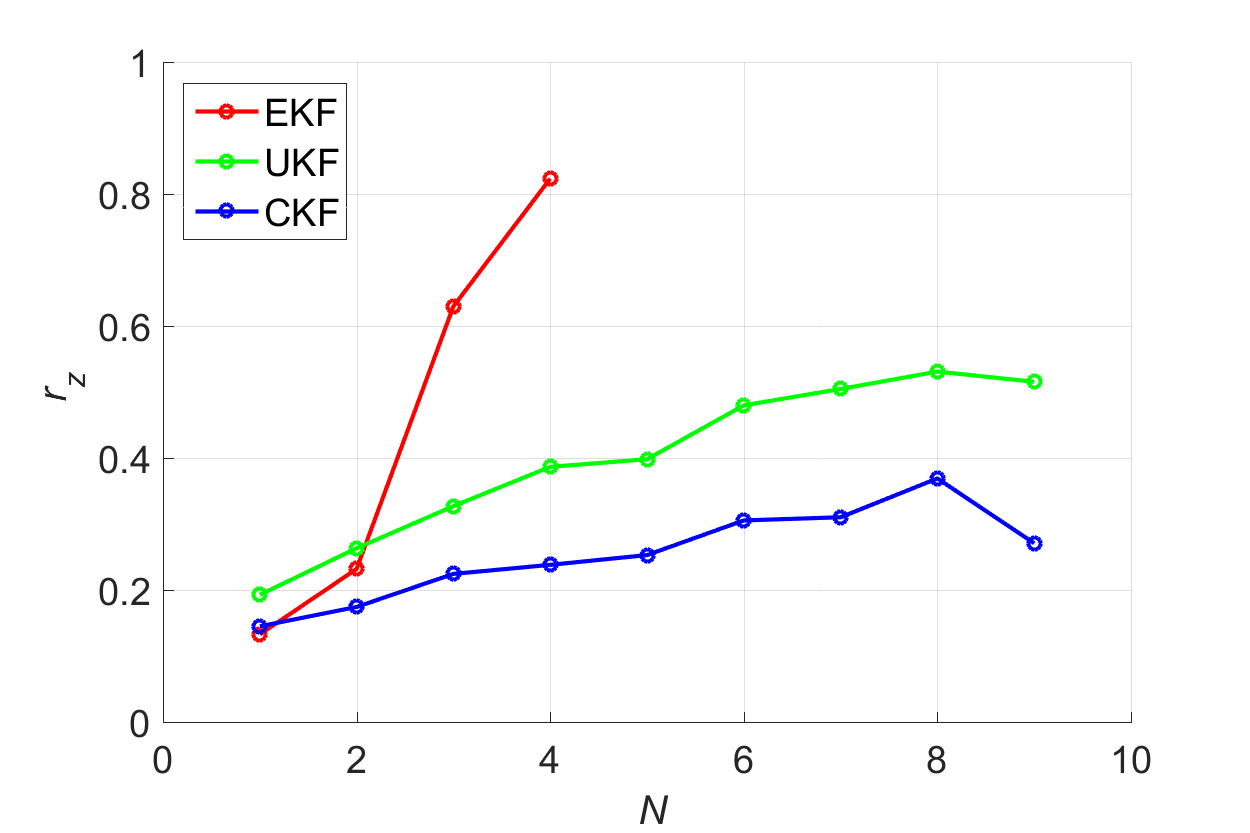
\includegraphics[height=0.2\textheight]{estcmpr_1} \\ а)}
	\end{minipage}
	\hfill
	\begin{minipage}[h]{0.49\linewidth}
		\center{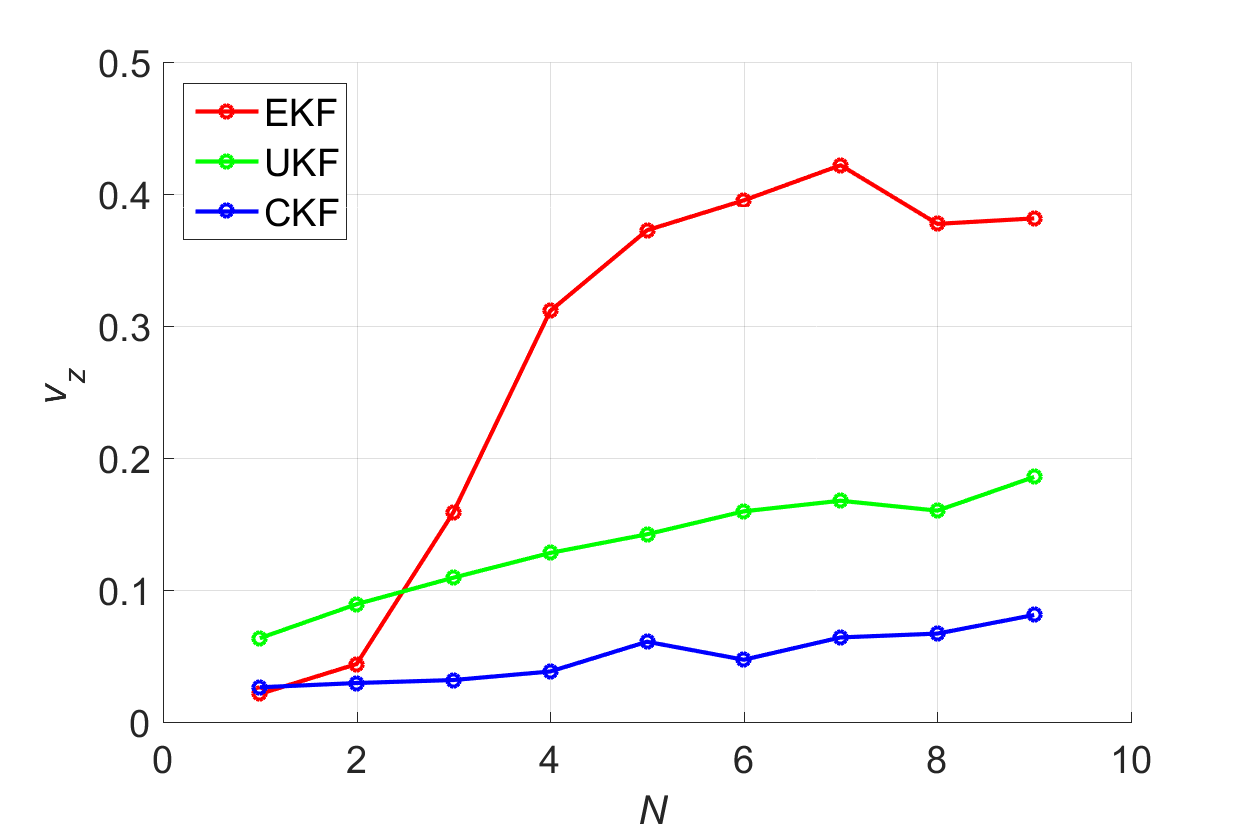
\includegraphics[height=0.2\textheight]{estcmpr_2} \\ б)}
	\end{minipage}
	\\
	\begin{minipage}[h]{0.49\linewidth}
		\center{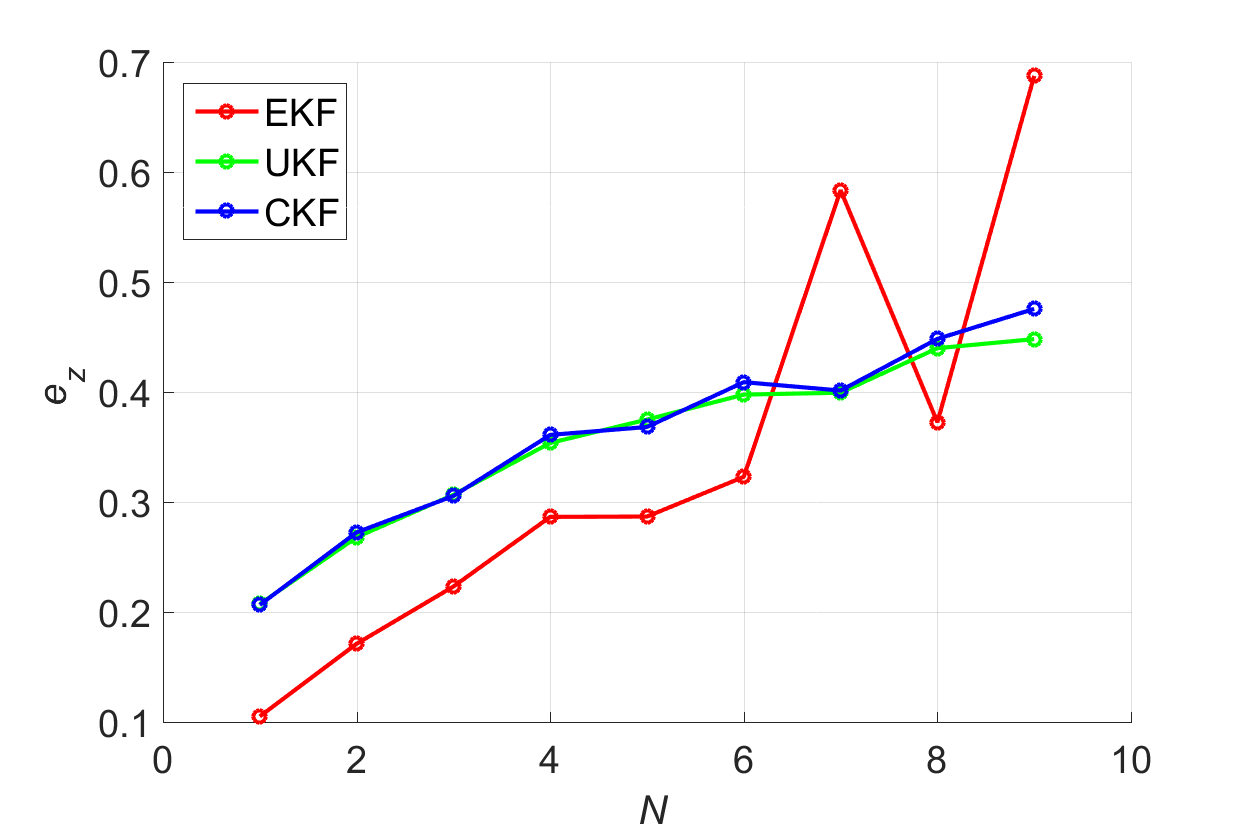
\includegraphics[height=0.2\textheight]{estcmpr_3} \\ а)}
	\end{minipage}
	\hfill
	\begin{minipage}[h]{0.49\linewidth}
		\center{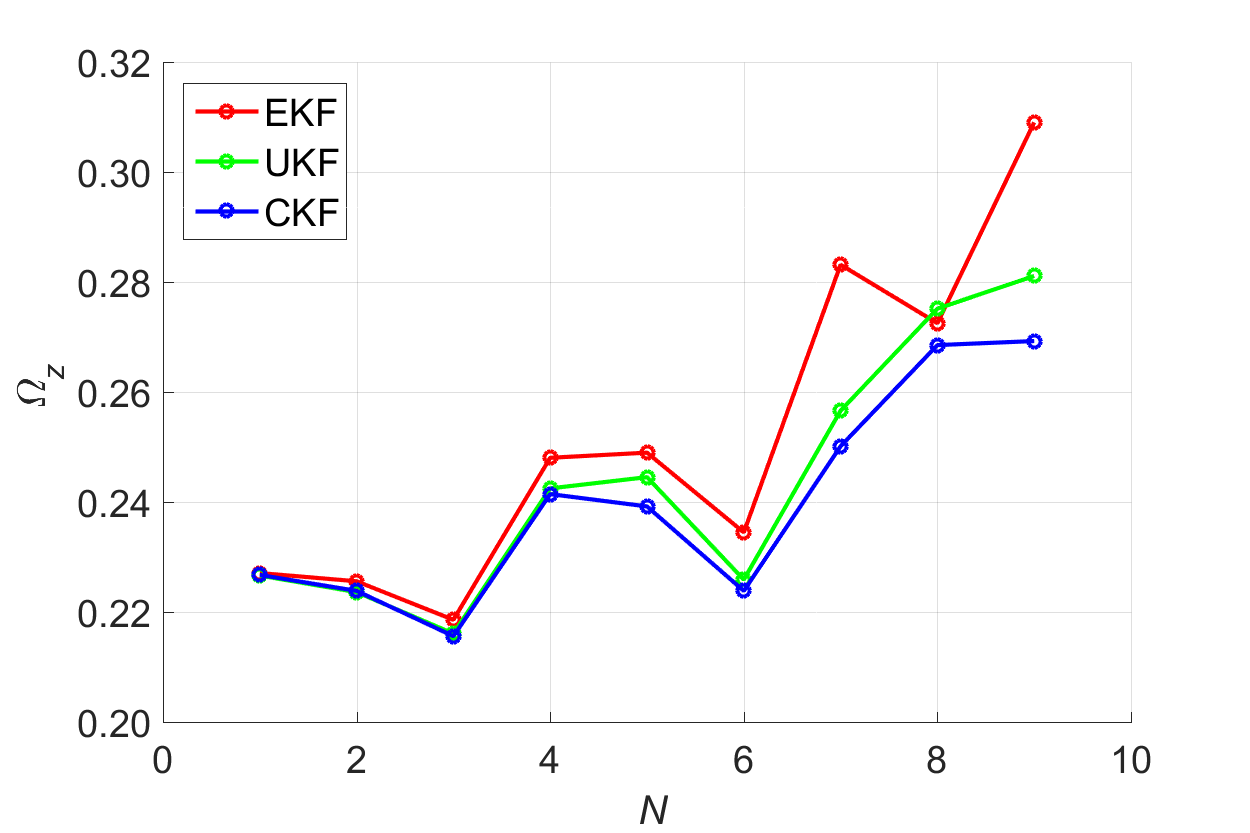
\includegraphics[height=0.2\textheight]{estcmpr_4} \\ б)}
	\end{minipage}
	\caption{Сравнение производительности алгоритмов фильтрации}
    \label{fig:est_cmpr}
\end{figure}

Превосходство UKF и CKF над EKF в этом экспериминте
обусловлено использованием в последнем из алгоритмов
линеаризованного уравнения стохастической дифференциальной системы \eqref{eq:m_dyn},
что негативно влияет на производительность метода при росте интервала измерений. Таким образом для системы управления квадрокоптером с поворотными роторами выбран кубатурный фильтр Калмана.

\section{Использование алгоритмов оценки состояния для идентификации параметров БЛА}

Эффективность работы системы управления напрямую зависит от качества оценки параметров динамики БЛА.
Если используемый регулятор не расчитан на работу в условиях неопределнности, ошибки в значениях используемых в системе управления ключевых констант могут привести к увеличению времени сходимости траектории к целевой, статическим ошибкам или даже потере устойчивости.
Так как в исследовании в основе контура управления лежит ПД-регулятор \ref{eq:m_reg}, необходимо как можно лучше идентифицировать параметры модели. 

Некоторые из динамических свойств объекта, такие как общая масса или физические размеры, измерить достаточно просто, для измерения других параметров требуется проводить достаточно трудоемкие операции.
Например, чтобы определить аэродинамические коэффициенты пропеллеров
$k$ и $b$
из выражений для внешних сил и моментов \ref{eq:m_dyn}, действующих на БЛА,
нужно демонтировать двигатель и использовать специальный стенд; такой способ применяют, например, в работе \cite{Ryll01}. При этом, например из-за микроповреждений пропеллеров, со временем эти параметры неизбежно изменятся и операцию придется повторять снова.

Отличной альтернативой является использование расширенного фильтра Калмана, с помощью которого возможно определять или уточнять некоторые параметры динамики квадрокоптера. Например, чтобы оценить аэродинамические константы $k$ и $b$, используем их как составляющие вектора состояния, вместе со скоростью и угловой скоростью:
\begin{equation}
\bm x = (\bm v^I, \bm \Omega^B, k, b)^T.
\end{equation}
При этом в качестве вектора измерений будем использовать
\begin{equation}
\bm z = (\bm v^I, \bm \Omega^B, \dot{\bm v^I}, \dot{\bm \Omega^B})^T.
\end{equation}
Как показывают эксперименты, в результате простого маневра -- взлета и разворота на $\frac{\pi}{2}$, который аппарат сможет выполнить относительно успешно даже с приблизительно известными параметрами, оценка коэффициентов $k$ и $b$
сходится к реальной. Известные параметры модели перечислены в Таблице \ref{tb:observer_params} , графики, демонстрирующие сходимость оценки к реальным значениям на рисунке \ref{fig:observer_k_b}, где красной линией изображена оценка, зеленой -- начальное приблизительное значение, синей -- истинное значение модели.
\begin{figure}[h!]
	\centering
	\subfloat[Оценка аэродинамического коэффициента пропеллера $k$]{%
		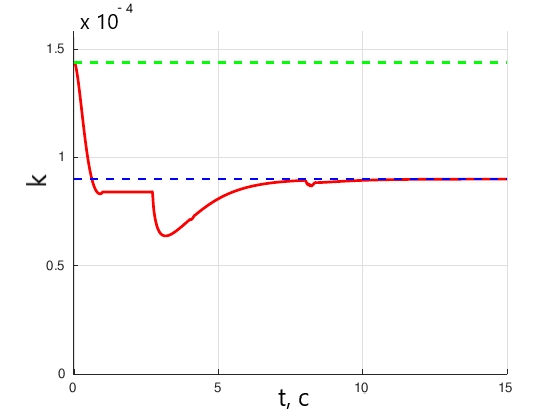
\includegraphics[clip,width=0.44\columnwidth]{k}%
	}
	\quad
	\subfloat[Оценка аэродинамического коэффициента пропеллера $b$]{%
		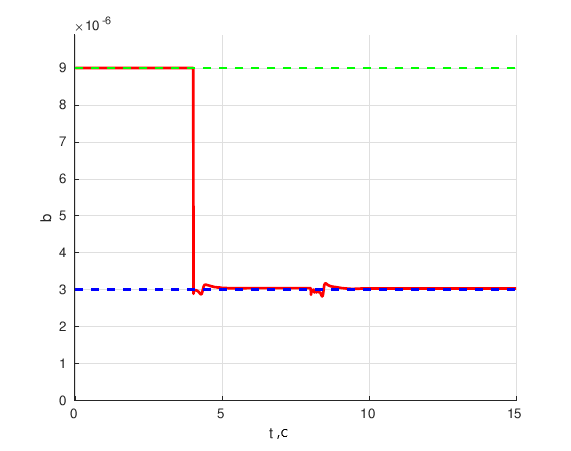
\includegraphics[clip,width=0.44\columnwidth]{b}%
	}
	\caption{ -- Уточнение параметров динамики БЛА}
	\label{fig:observer_k_b}
\end{figure}
\begin{table}[ht]
	\centering
	\caption{ -- Известные параметры модели}\label{tb:observer_params} 
	\begin{tabular}{lcl}
		\hline
		Параметр & Обозначение & Значение  \\\hline
		Общая масса & $M$ & 3,6 кг  \\
		Тензор инерции корпуса & $\bm J_B$ & $diag(53, 63, 98) \cdot{10^{-3}}$ кг$\cdot$м$^2$  \\
		Тензор инерции ротора & $\bm J_R$ & $diag(85, 85, 46) \cdot{10^{-6}}$ кг$\cdot$м$^2$  \\
		Миделево сечение корпуса & $S_{\perp}$ & 0,2 м$^2$ \\
		Луч & $L$ & 0,35 м \\
		Аэродинамический коэффициент & $C$ & 1,05\\	
		Максимальные обороты & $\tilde \omega_{max}$ & 500 рад/с \\		
		Максимальный угол & $\theta_{max}$ & ${\pi}/{4}$ рад \\
		\hline
	\end{tabular}
\end{table}

	
\chapter{Численные эксперименты}
\label{experiments_chapter}

\section{Структура модели}

Для подтверждения работоспособности синтезированной системы управления разработанные алгоритмы реализованы в прикладном пакете Matlab Simulink; модель состоит из четырех основных блоков (см. рисунок \ref{fig:simulink_scheme}):
\begin{itemize}
	\item Блок «СТФК» реализует описанные в главе \ref{chapter_estimation} алгоритмы оценки состояния; на его вход поступают измерения бортовых датчиков, затем оценка текущего состояния используется модулем "управление"
	\item Блок «управление» использует обращенную модель динамики аппарата \ref{eq:m_dyn_resolve} для вычисления вектора управляющих воздействий на основе текущих и целевых параметров движения с учетом введеных ограничений \ref{eq:m_limits_init};
	\item Блок «модель» интегрирует движение системы на основе модели
	(\ref{eq:m_vel}), (\ref{eq:m_puasson}), (\ref{eq:m_traslational_motion}) и (\ref{eq:m_final_rotational_motion})
	и управляющего воздействия.
	\item Блок «датчики» использует результаты интегрирования движения БЛА для моделирования показаний датчиков.
\end{itemize}
\begin{figure}[h!]
	\centering
	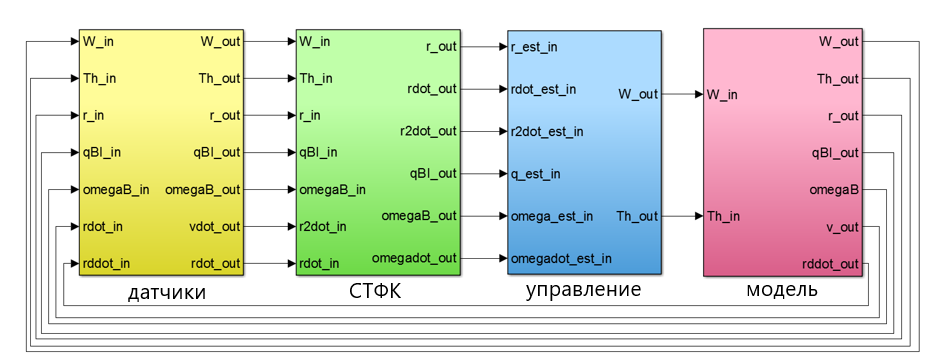
\includegraphics[width=16cm]{simulink_scheme}
	\caption{ -- Общая схема численной модели}
	\label{fig:simulink_scheme}
\end{figure}
В качестве численных методов для моделирования движения БЛА используется метод Рунге-Кутты 4-го порядка с шагом интегрирования $dt={10^{-3}}$c.

\section{Параметры управляемой динамики БЛА и соответствующие им ограничения}

Маневренные возможности любого летательного аппарата напрямую зависят от основных параметров его динамики.
Они, в свою очередь, ограничены множеством доступных для проектирования летательного аппарата подсистем, таких, как подсистема эноргообеспечения, подсистема исполнительных органов управления, вычислительная система и другие. 
В работе, с учетом сформулированных в разделе \ref{section_ctrl_task} задач управления, для эксперимента выбраны параметры, соответсвующие небольшому квадрокоптеру, способному нести на борту дополнительную нагрузку в виде камеры высокого разрешения и использующему в качестве источника питания малогабаритную электрическую батарею; они приведены в Таблице \ref{tb:params_table}.
\begin{table}[h!]
	\centering
	\caption{ -- Параметры модели}\label{tb:params_table} 
	\begin{tabular}{lcl}
		\hline
		Параметр & Обозначение & Значение  \\\hline
		Общая масса & $M$ & 2 кг  \\
		Тензор инерции корпуса & $\bm J_B$ & $diag(2,\ 2,\ 4)\cdot{10^{-2}}$ кг$\cdot$м$^2$  \\
		Тензор инерции ротора & $\bm J_R$ & $diag(2,\ 2,\ 1)\cdot{10^{-5}}$ кг$\cdot$м$^2$  \\
		Миделево сечение корпуса & $S_{\perp}$ & 0,12 м$^2$ \\
		Луч & $L$ & 0,25 м \\
		Аэродинамический коэффициент & $C$ & 1,05\\
		Аэродинамический коэффициент & $k$ & 1,13$\cdot 10^{-5}$ Н$\cdot$с$^2\cdot$рад$^{-2}$ \\		
		Аэродинамический коэффициент & $b$ & 1,5$\cdot 10^{-6}$ Н$\cdot$м$\cdot$с$^2\cdot$рад$^{-2}$ \\		
		Максимальные обороты & $\tilde \omega_{max}$ & 1140 рад/с \\		
		Максимальный угол & $\theta_{max}$ & ${\pi}/{3}$ рад \\
		Константа балансировки & $\varepsilon_\tau$ &6 Н$\cdot$м \\
		\hline
	\end{tabular}
\end{table}

Эти параметры использовались для рассчета ограничений на выходы регулятора \eqref{eq:m_reg} с использованим алгоритма, описанного в разделе \ref{section:limits}. Сначала было выбрано направление диагонали прямоугольной области $\Psi_{\boldsymbol{y}}$ таким образом, чтобы ограничения на выход регулятора \eqref{eq:m_reg} позволяли решать поставленные в эксперименте задачи. 
Для рассматриваемой конфигурации, описанной в Таблице \ref{tb:params_table}, выберем
$$\bm d = (0,577, 0,577, 0,577, 0,014, 0,014, 0,014).$$
Для выбранной диагонали найдем значения пределов ограничений \eqref{eq:lims_final} и балансировочных параметров, входящих в дополняющие модель \eqref{eq:m_dyn} уравнения \ref{eq:m_dyn_balance_1}, \ref{eq:m_dyn_balance_2}. Результаты приведены в Таблице \ref{tb:lims_table}.
\begin{table}[h!]
	\centering
	\caption{Параметры ограничений}\label{tb:lims_table} 
	\begin{tabular}{lcl}
		\hline	
		Длина диагонали & $2\gamma^*$ & $28$ \\
		Константа балансировки & $\varepsilon_T$ &2,6 Н$\cdot$м \\
		Константа балансировки & $\varepsilon_F$ &0 Н\\
		\hline
	\end{tabular}
\end{table}
Таким образом выполнение имеющихся ограничений параметров системы исполнительных органов управления на максимальные обороты двигателей
$\tilde \omega_{max}$ = 1140 рад/с
и на максимальные углы отклонения роторов с пропелерами от вертикали
$\theta_{max}$ = ${\pi}/{3}$ рад,
ограничивает максимально возможнок целевое ускорение БЛА по каждой из осей значением
$\ddot {\bm r}_{max}^0 \approx 4$ м/с$^2$,
угловое ускорение вдоль осей $X$ и $Y$ значением
$\dot {\bm \Omega}_{max}^0 \approx 10$ рад/с$^2$
и угловое ускорение вдоль оси $Z$ значением
$\dot {\tilde{\bm \Omega}}_{max}^0 \approx 5$ рад/с$^2$.

\section{Модель бортовых датчиков и параметры кубатурного фильтра Калмана}

Для обеспечения обратных связей в контуре управления, как было отмечено в главе \ref{chapter_estimation}, в качестве алгоритма оценки состояния был выбранкубатурный фильтр Калмана, использующий в качестве вектора состояния
\begin{equation}
\bm x = (\bm r^I, \bm v^I, q_BI, \bm \Omega^B)
\end{equation}
и соответсвующие измерения
\begin{equation}
\bm z = (\bm r^I, \bm v^I, q_BI, \bm \Omega^B).
\end{equation}
В эксперименте в качестве основы для моделирования показаний бортовых сенсоров использована реально существующая и популярная среди разработчиков мультироторных роботов бортовая система Xsens MTi-7 \cite{xsens01}.
Она содержит стандартный набор необходимых для оценки состояния БЛА подсистем, включающих себя спутниковую систему глобального позиционирования, цифровой барометрический датчик давления, трехосевые электромеханические акселерометр и гироскоп, а также магнитный компас.
Устройством предусмотрена возможность автоматической калибровки датчиков для устранения статических ошибок, которые могут возникнуть при его установке.

Измерения датчиков моделируются добавлением к результатам интегрирования уравнений движения БЛА белого гауссовского шума с параметрами, соответствующими значениям, указанным в документации устройства \cite{xsens01}.
Показания угловой скорости также содержат составляющую, отвечающую за дрейф нуля датчика угловой скорости.
Стандартные отклонения для шума измерений горизонтальной составляющей позиции, вертикальной составляющей позиции, скорости, угла тангажа, крена и рысканья приведены в таблице \ref{tb:exp_noise_params}, плотность шума измерений угловой скорости равна  
${{{\rho }}_{^{{\Omega }}}} = 7\cdot{10^{-3}}$ с$^{-1}$ $\sqrt{\text{Гц}}$,
а дрейф нуля
${{\beta }}_{^{{\Omega }}} = 3\cdot{10^{-3}}$ с$^{-1}$.
\begin{table}[h!]
	\caption{ -- Параметры шума измерений}\label{tb:exp_noise_params} 
	\centering
	\begin{tabular}{|>
			{\centering\arraybackslash}m{1.5in}|>
			{\centering\arraybackslash}m{1.5in}|}
		\hline
		${{{\sigma }}_{rx}}$& 1м \\ \hline
		${{{\sigma }}_{rz}}$& 2м \\ \hline
		${{{\sigma }}_{v}}$& 0.5м/с \\ \hline
		${{{\sigma }}_{\alpha}}$& 0.5$^\circ$ \\ \hline
		${{{\sigma }}_{\beta}}$& 0.5$^\circ$ \\ \hline
		${{{\sigma }}_{\gamma}}$& 1.5$^\circ$ \\ \hline
	\end{tabular}
\end{table}
Для выбранных датчиков были выбраны
ковариационная матрицы шума системы и шума измерений
$\bm Q$,
$\bm R$,
из выражений \eqref{eq:ukf_p_apr}, \eqref{eq:ukf_s_k}
\small
\begin{equation}
\begin{aligned}
&\bm Q = diag(1,\ 1,\ 2,\ {10^{-1}}, {10^{-1}}, {10^{-1}}, {10^{-2}}, {10^{-4}}, {10^{-4}}, {10^{-4}}, {10^{-2}}, {10^{-2}}, {10^{-2}}),
\\
&\bm R = diag({10^{-2}}, {10^{-2}}, {10^{-2}}, {10^{-2}}, {10^{-2}}, {10^{-2}}, {10^{-6}}, {10^{-6}}, {10^{-6}}, {10^{-6}}, {10^{-2}}, {10^{-2}}, {10^{-2}}).
\end{aligned}
\end{equation}
\normalsize

\section{Эксперимент: наблюдение за подвижным объектом}

В эксперименте аппарат должен выполнить наблюдение за подвижным объектом, летя неподалеку от него и ориентируя камеру, установленную спереди, так, чтобы объект находился в центре полученного изображения.
Мы не рассматриваем вопрос построения траектории БЛА, считая ее определённой заранее.
Точка старта аппарата расположена на расстоянии 90 метров от цели, затем оно постепенно сокращается до 50 метров.
Траектория БЛА и наблюдаемого объекта изображены на рисунке \ref{fig:mau_traj}.
\begin{figure}[H]
	\centering
	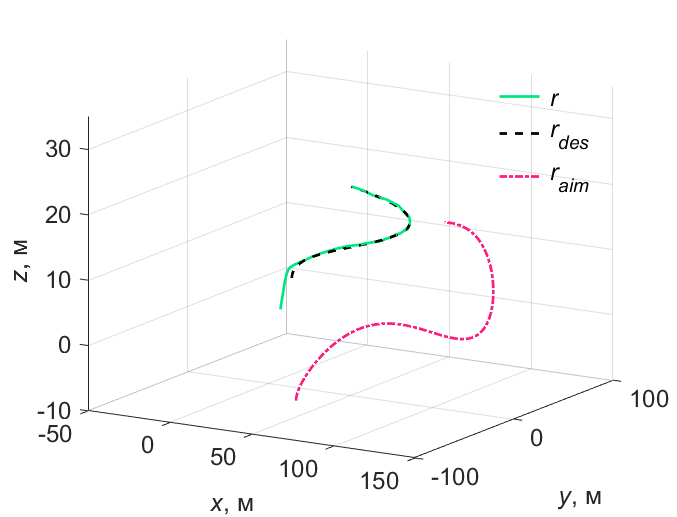
\includegraphics[width=14cm]{traj.png}
	\caption{ -- Траектория БЛА и объекта наблюдения}
	\label{fig:mau_traj}
\end{figure}

На рисунке \ref{fig:mau_errors}, на графиках слева, изображены ошибки ориентации по углам крена, тангажа и рысканья,
а справа -- ошибки положения  квадрокоптера по осям $X$, $Y$ и $Z$.
Ошибки по каждому из углов ориентации после стабилизации не превышают одного градуса.
После выхода аппарата на целевую траекторию максимальное абсолютное отклонение от траектории составило 30 см.
\begin{figure}[H]
	\centering
	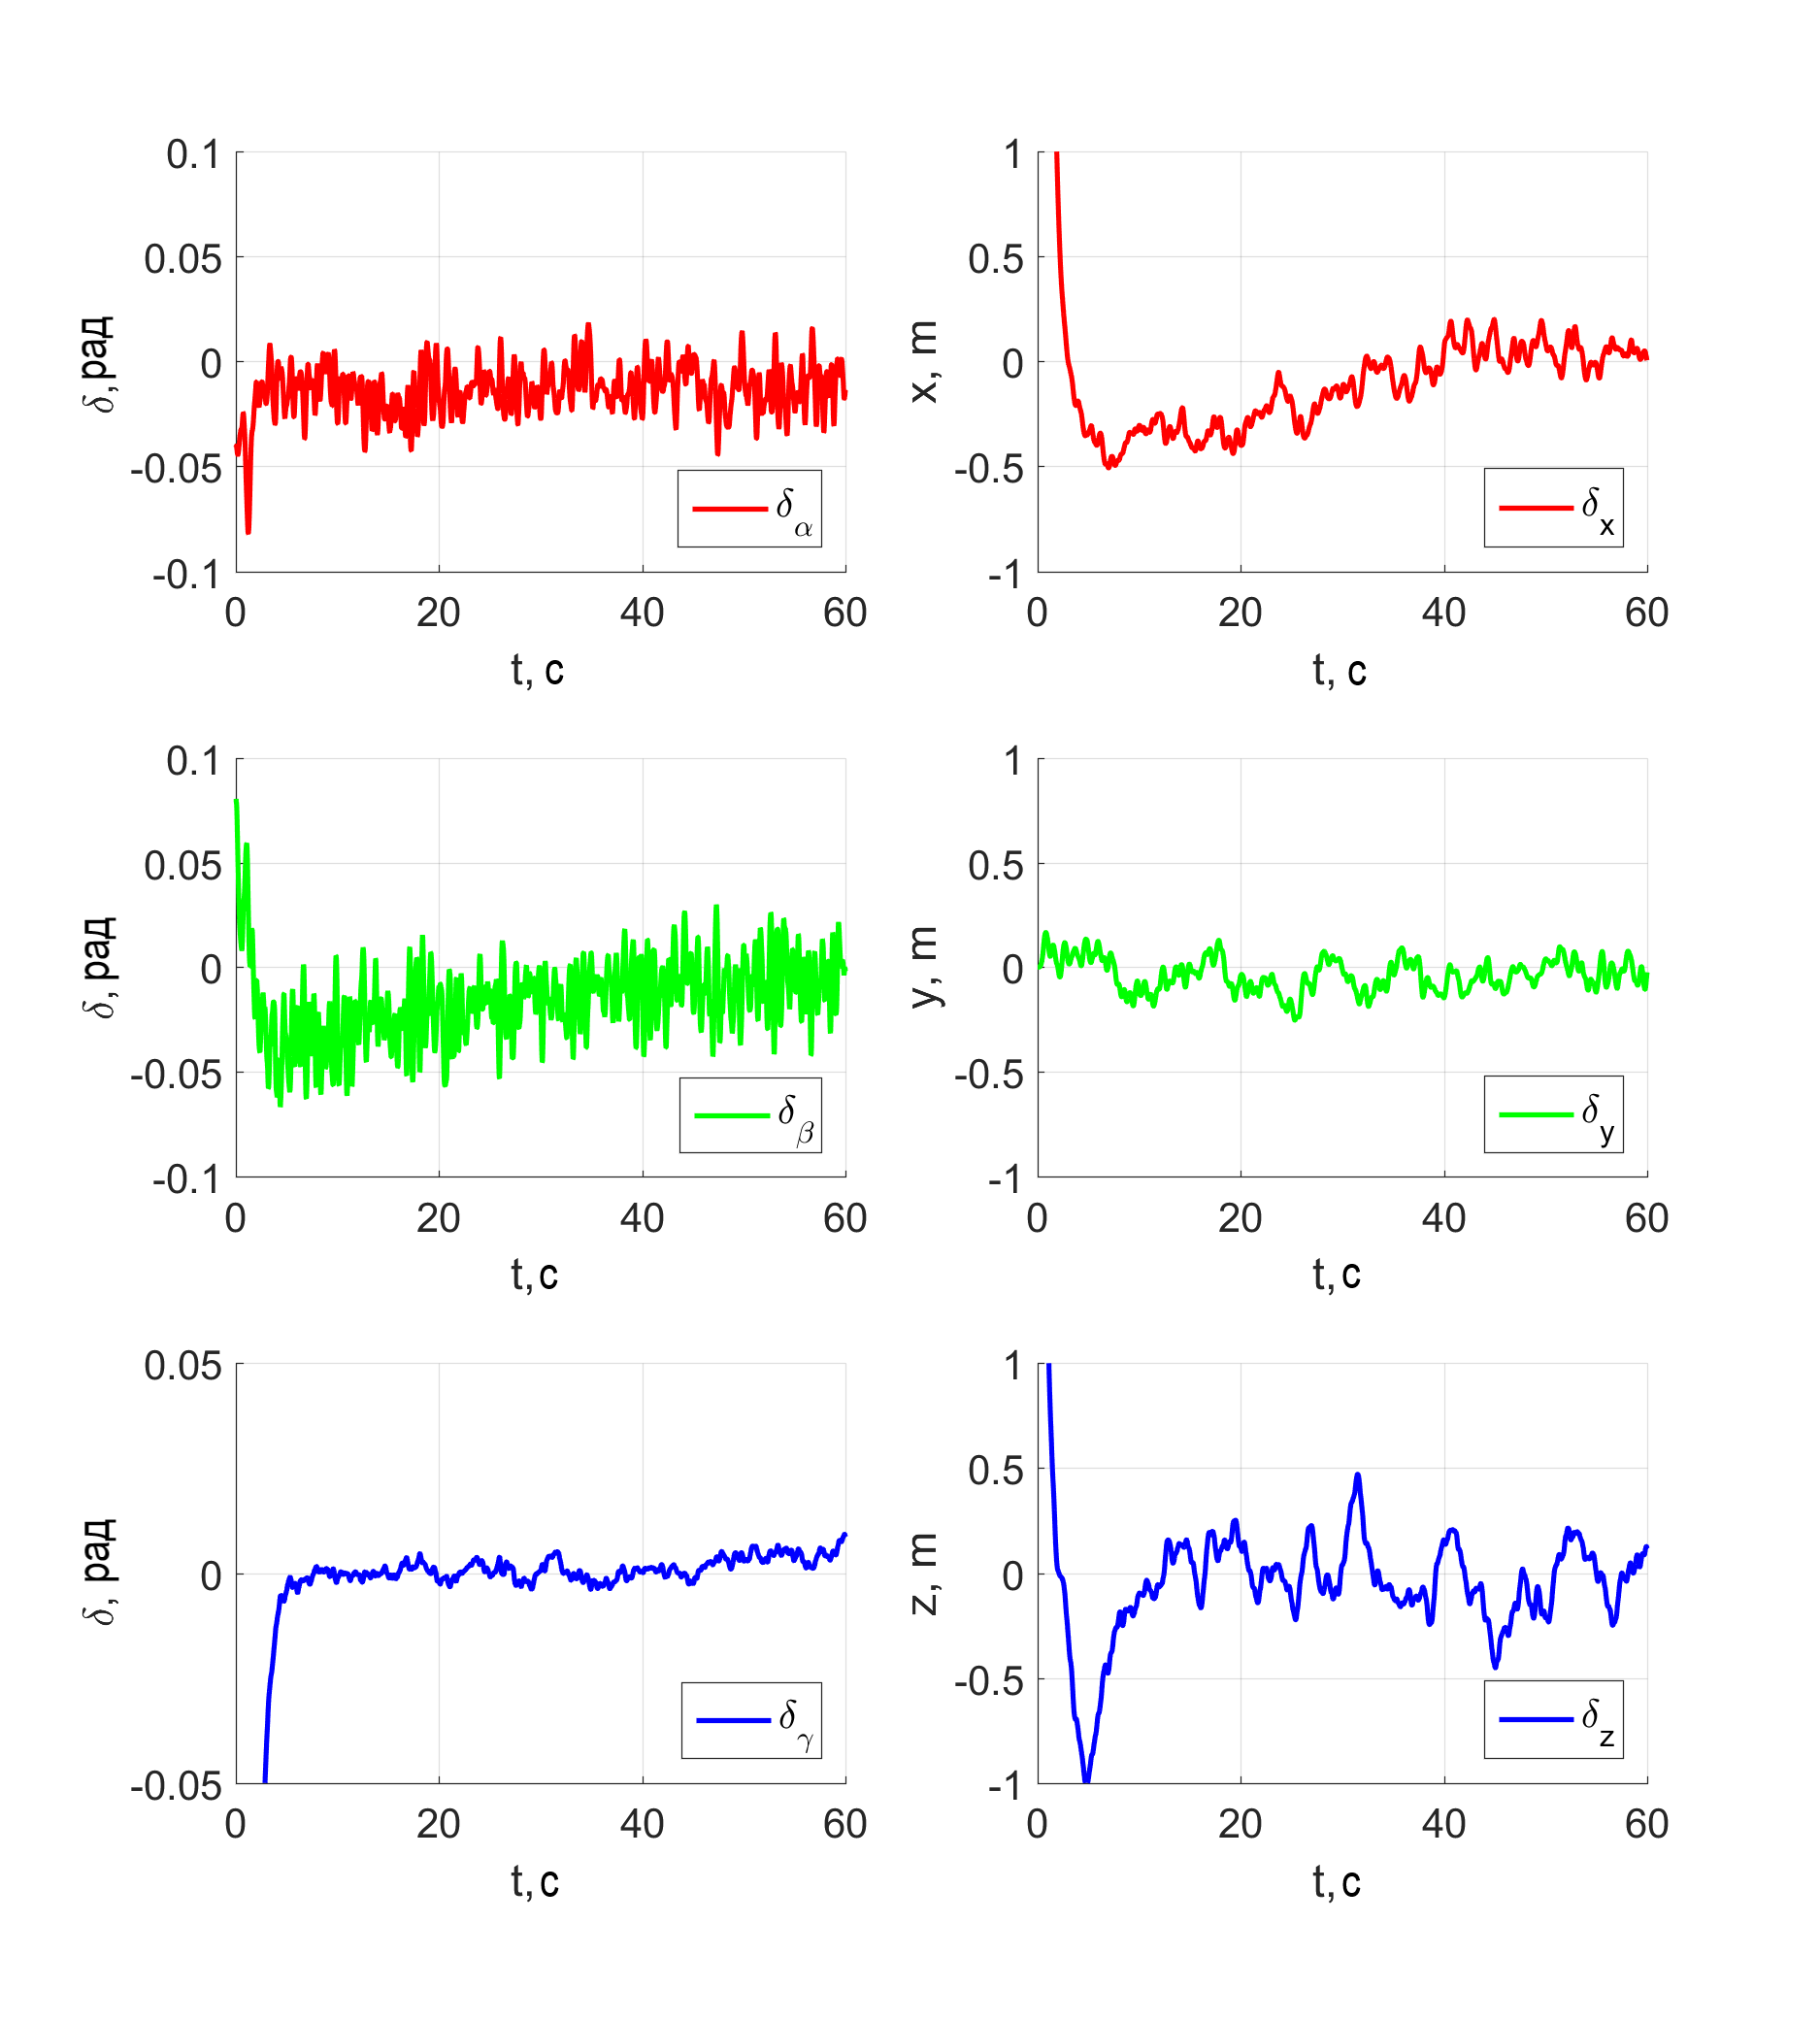
\includegraphics[width=14cm]{errors_rows.png}
	\caption{ -- Отклонение параметров движения БЛА от целевых значений}
	\label{fig:mau_errors}
\end{figure}

На рисунке \ref{fig:mau_cam} можно проследить за траекторией наблюдаемого объекта на записи, которою можно сделать с помощью передней камеры.
Видно, что в начальный момент времени объект находится вне зоны видимости, затем перемещается в центр экрана и далее на протяжении всего времени манёвра ось визирования камеры отклоняется от направления на объект не более чем на 1$^\circ$.
\begin{figure}[H]
	\centering
	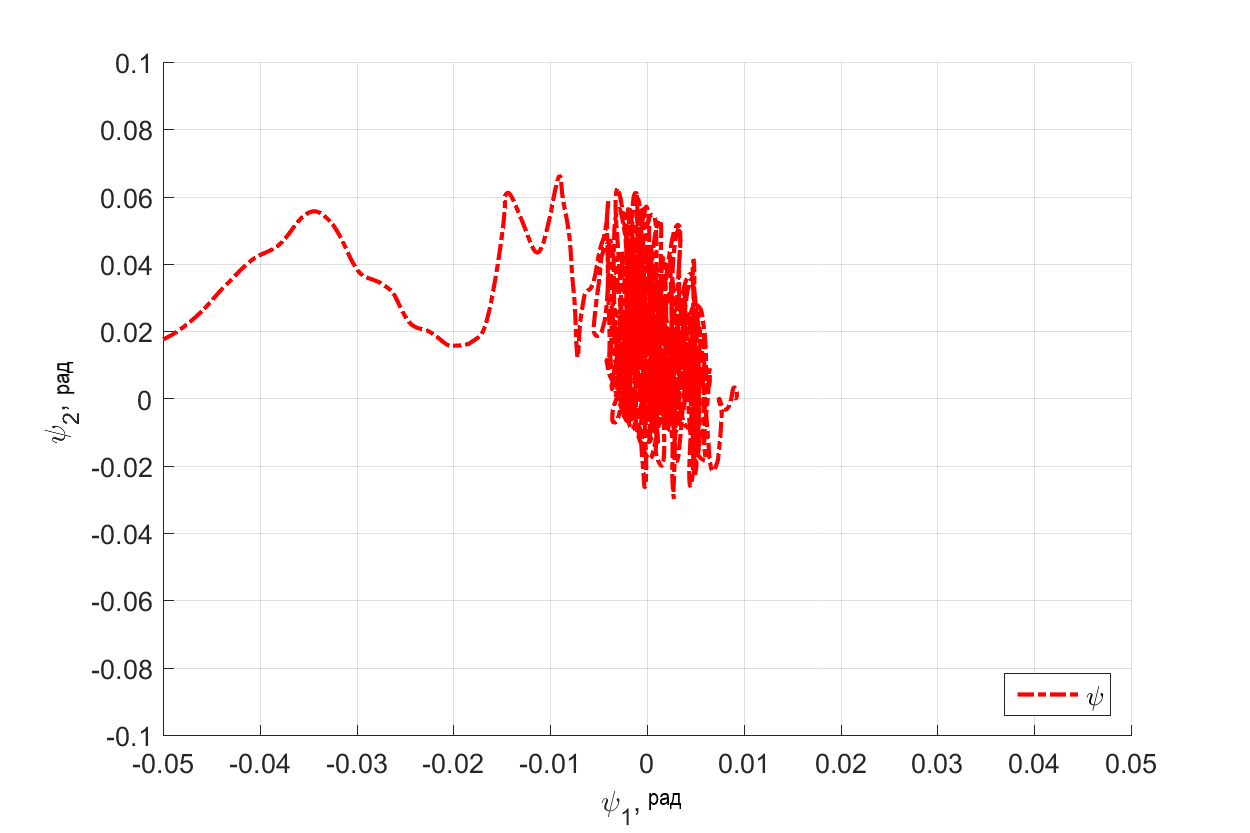
\includegraphics[width=14cm]{camera.png}
	\caption{ -- Траектория объекта на записи}
	\label{fig:mau_cam}
\end{figure}
Рисунок \ref{fig:mau_est} демонстрирует производительность алгоритмов оценки состояния. Слева приведены графики ошибки оценки углов крена, тангажа и рысканья и их прямых измерений. Справа – оценка положения по осям $X$, $Y$ и $Z$  и их прямые измерения.
\begin{figure}[H]
	\centering
	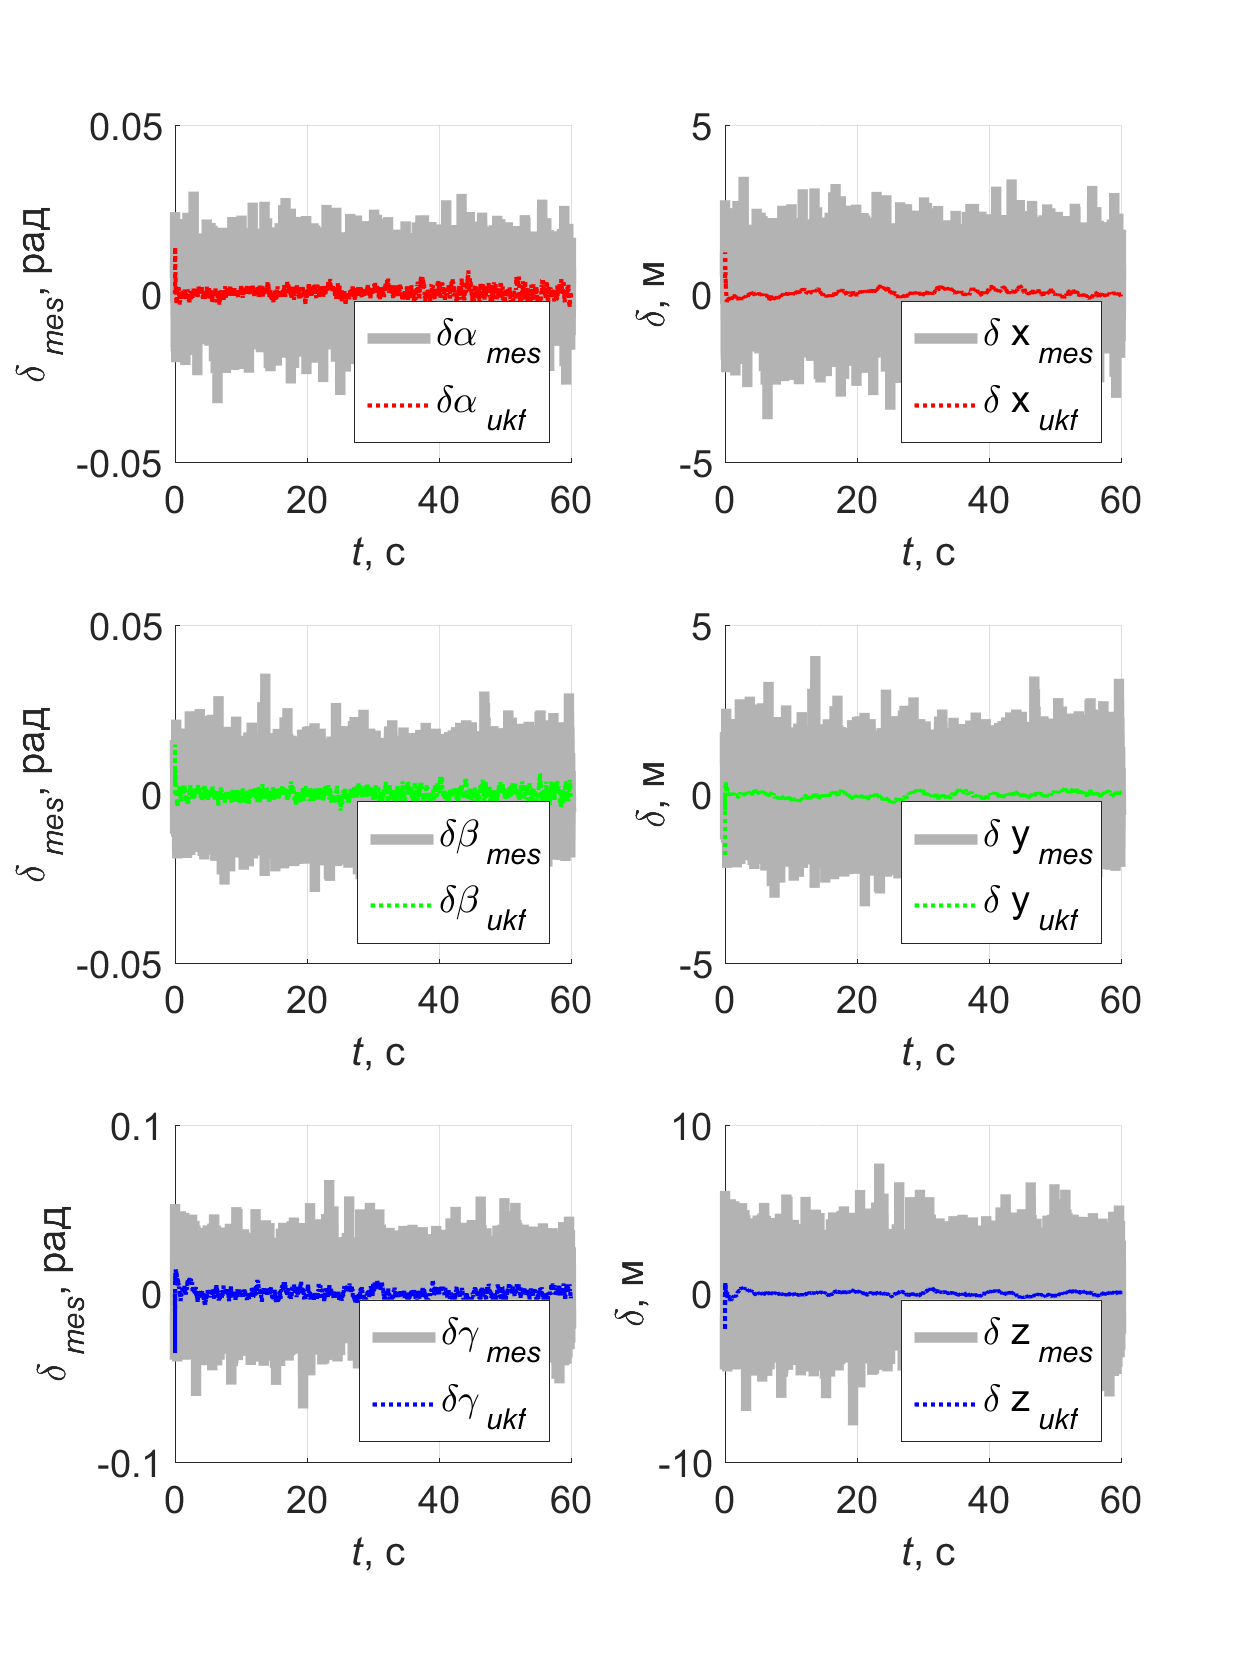
\includegraphics[width=14cm]{ukf_perf_raws.png}
	\caption{ -- Ошибка оценки состояния и прямых измерений}
	\label{fig:mau_est}
\end{figure}
Алгоритмы фильтрации позволили значительно снизить уровень шума измерений.

На графиках, изображенных на рисунке \ref{fig:mau_ctrl_out} представлены компоненты вектора управляющих параметров, которые, как легко заметить, лежат внутри ограниченной предельными значениями области.

\begin{figure}[H]
	\centering
	\subfloat{%
		\subfloat[]{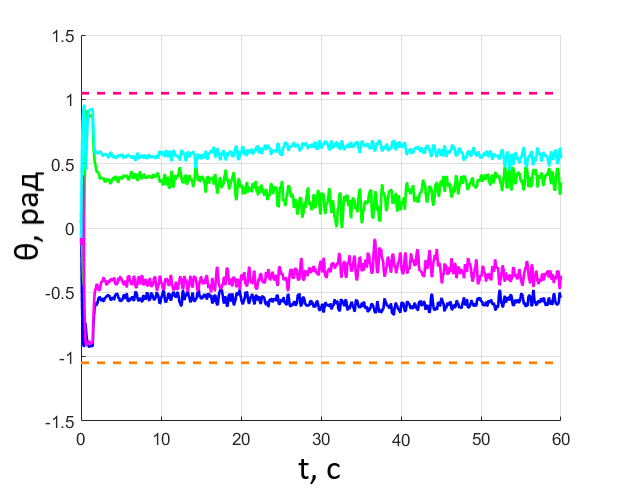
\includegraphics[clip,width=0.49\columnwidth]{rotor_angles}}%
		\subfloat[]{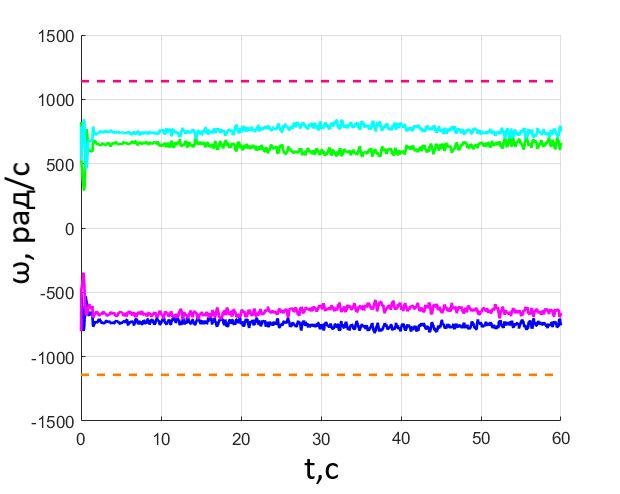
\includegraphics[clip,width=0.49\columnwidth]{rotor_rates}}%
	}
	
	\caption{ -- Управляющие параметры}
	\label{fig:mau_ctrl_out}
	
\end{figure}


В результате эксперимента мы оценили способность БЛА с поворотными роторами справляться со сложными маневрами, где необходимо независимо управлять ориентацией и положением аппарата. Квадрокоптер быстро вышел на целевую траекторию и успешно отслеживал ее, ориентируя бортовую камеру таким образом, чтобы объект наблюдения всегда оставался в центре изображения.
Стоит отметить, что при необходимости более точного отслеживания траектории имеет смысл использовать более чувствительные инструменты для измерения текущего положения и скорости, например, технологию RTK GPS \cite{Feng01}, где применение неподвижной наземной базовой станции уменьшает погрешность измерений на 1-2 порядка.


\section{Эксперимент: экстренная посадка}

В эксперементе рассматривается сценарий отказа двух смежных двигателей. Применяются алгоритмы управления, описанные в разделе \ref{section_em_ctrl}. Как было отмечено, для возможности применения системы экстренного управления необходим значительный запас тяги двигателей и более широкие пределы отклонений сервоприводов. Поэтому в эксперементе параметры ограничений БЛА несколько отличаются от тех, что представлены в таблице \ref{tb:params_table}, а именно
\begin{equation}
\begin{aligned}
&\tilde{\omega}_{max} = 1318 рад/c,
\\
&\theta_{max} = \pi.
\end{aligned}
\end{equation}

В начальный момент времени аппарат находится на высоте 25 метров недалеко от точки взлета.
При отказе двигателей начинается переход в режим экстренного управления.
За время менее 5 секунд высота БЛА упала более чем на 15 метров, но затем, когда аппарат стабилизиировал свою ориентацию около целевых значений, падение прекратилось и аппарат приступил к плавному снижению со скоростью около 0,5 метров в секунду с одновременным движением в сторону места своего запуска. По истечении 30 секунд квадрокоптер стабилизировал свое положение около точки взлета. На рисунке \ref{fig:em_coords} представлены параметры движения мультироторного робота в процессе экстренной посадки. Слева изображены графики компонент векторной части кватерниона ориентации корпуса, справа -- проекции координат центра масс БЛА на оси инерциальной системы отсчета.
\begin{figure}[H]
	
	\centering
	\subfloat[крен]{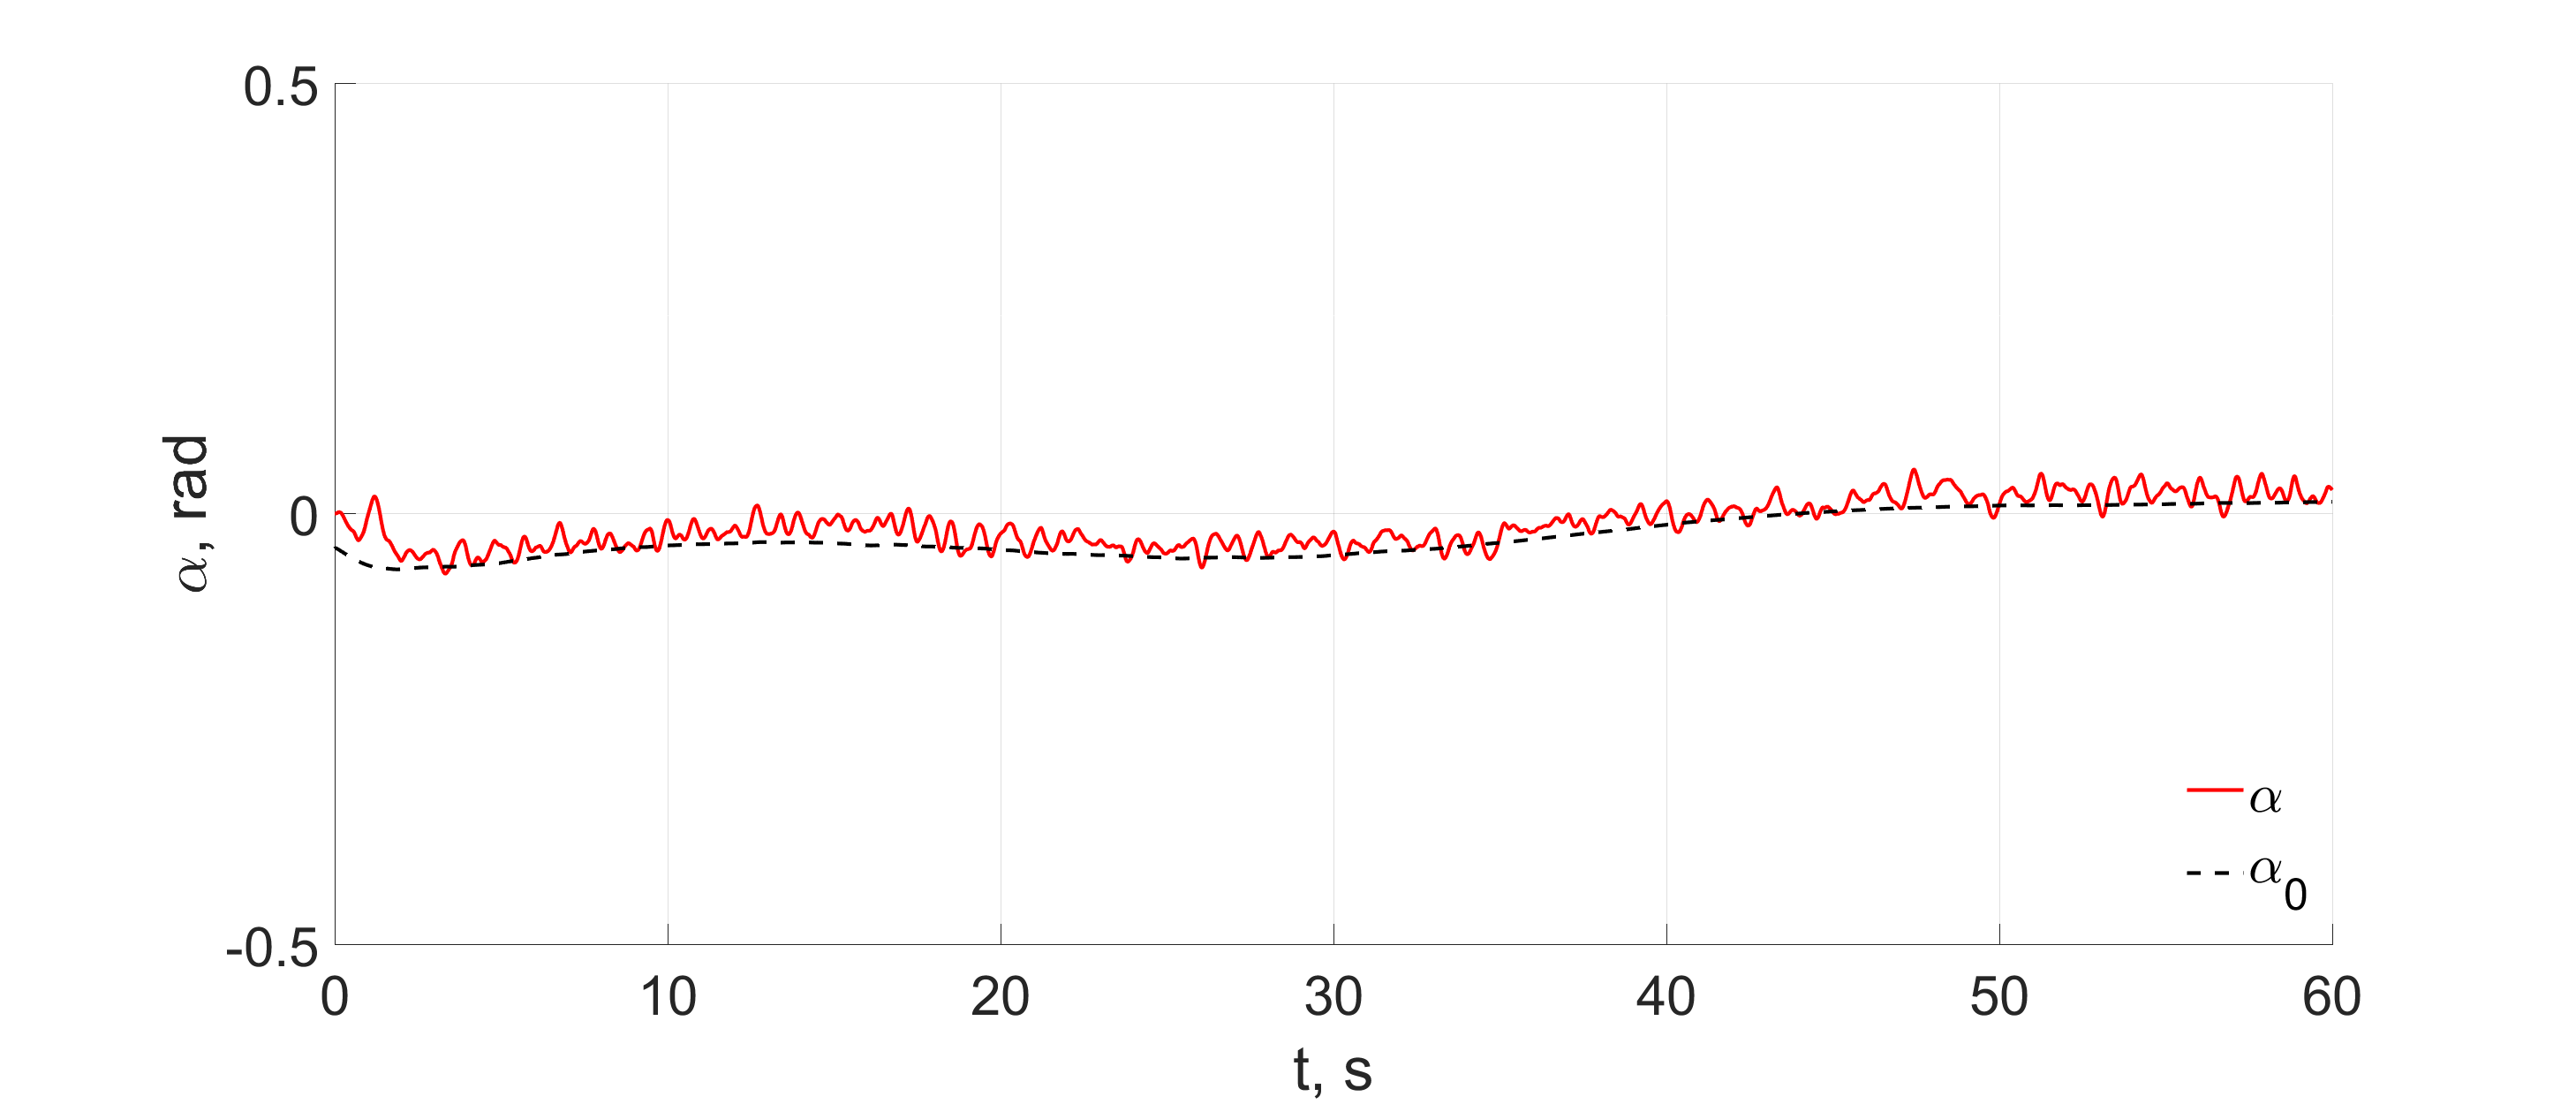
\includegraphics[width=8cm]{em/roll}}\hfil
	\subfloat[коордиата x]{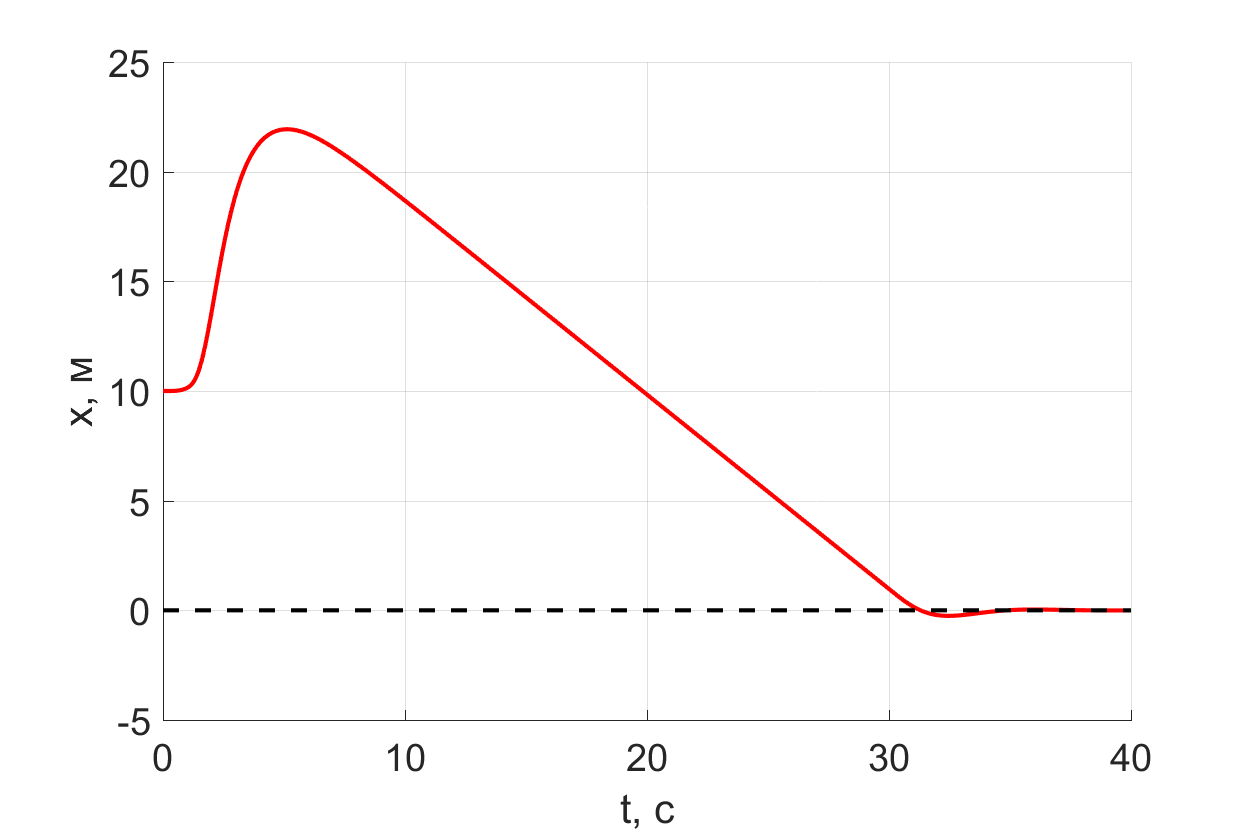
\includegraphics[width=8cm]{em/x}}
	
	\subfloat[тангаж]{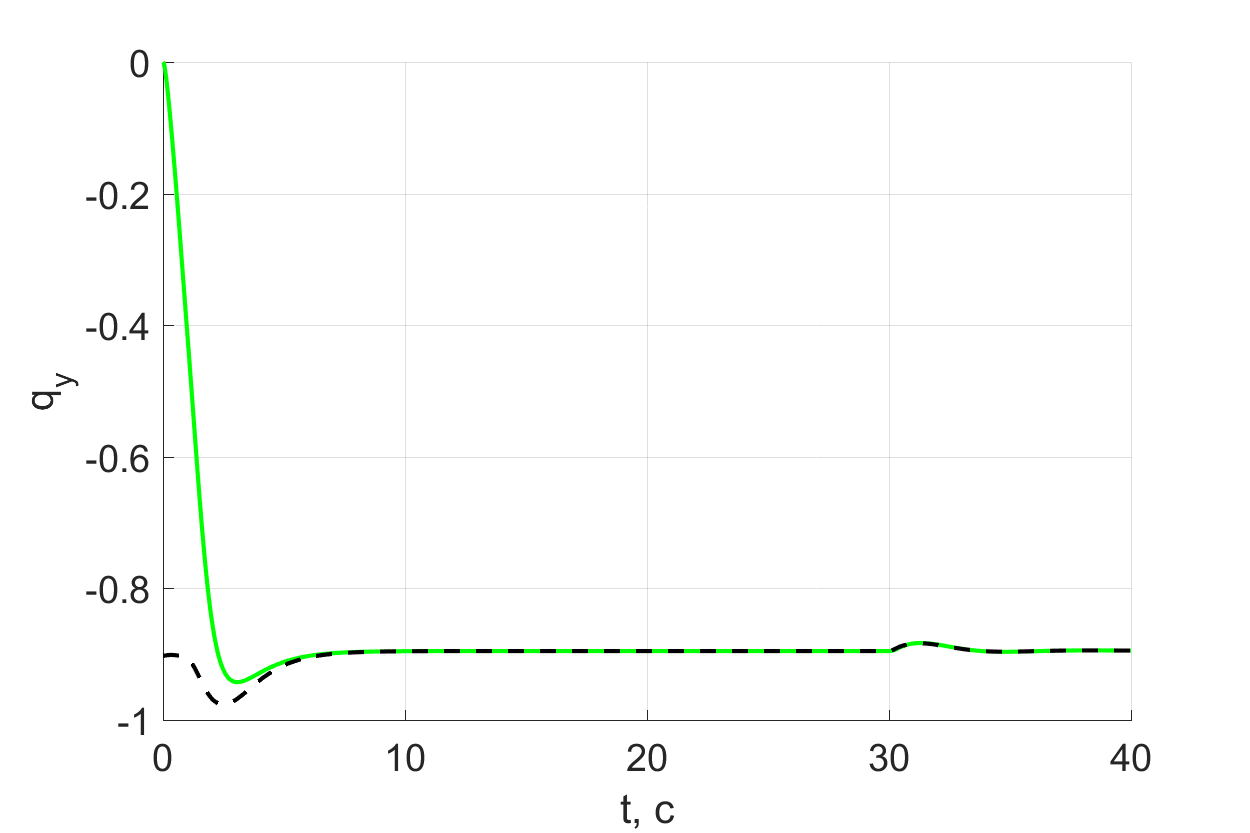
\includegraphics[width=8cm]{em/pitch}} \hfil 
	\subfloat[коордиата y]{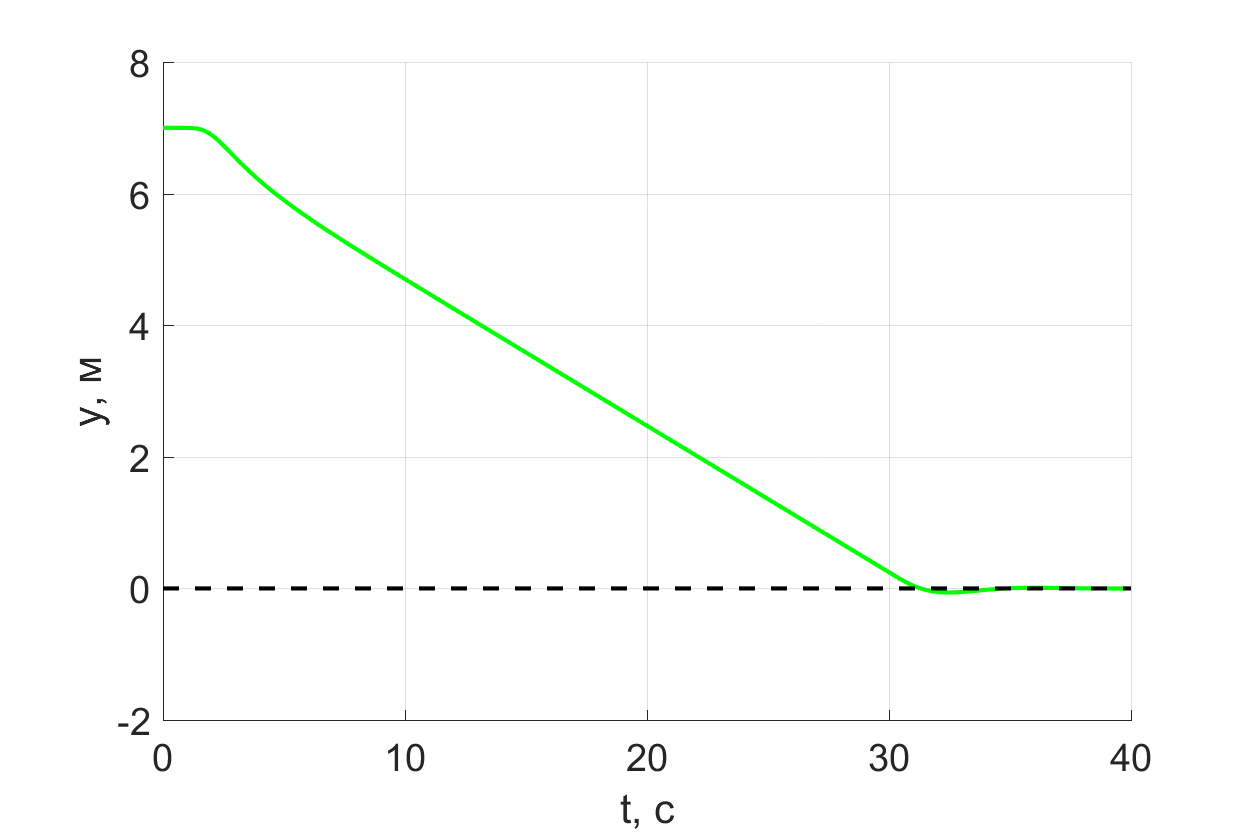
\includegraphics[width=8cm]{em/y}}  
	
	\subfloat[рысканье]{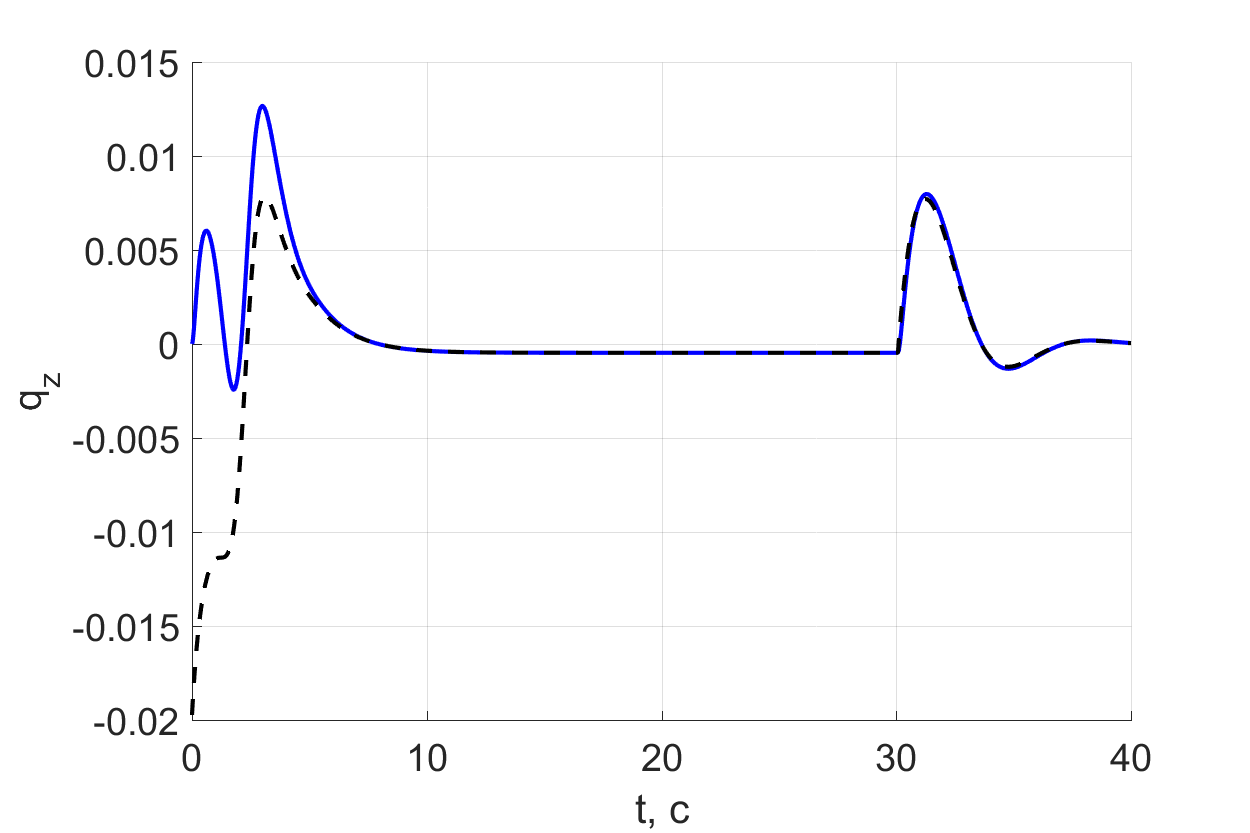
\includegraphics[width=8cm]{em/yaw}}\hfil
	\subfloat[коордиата z]{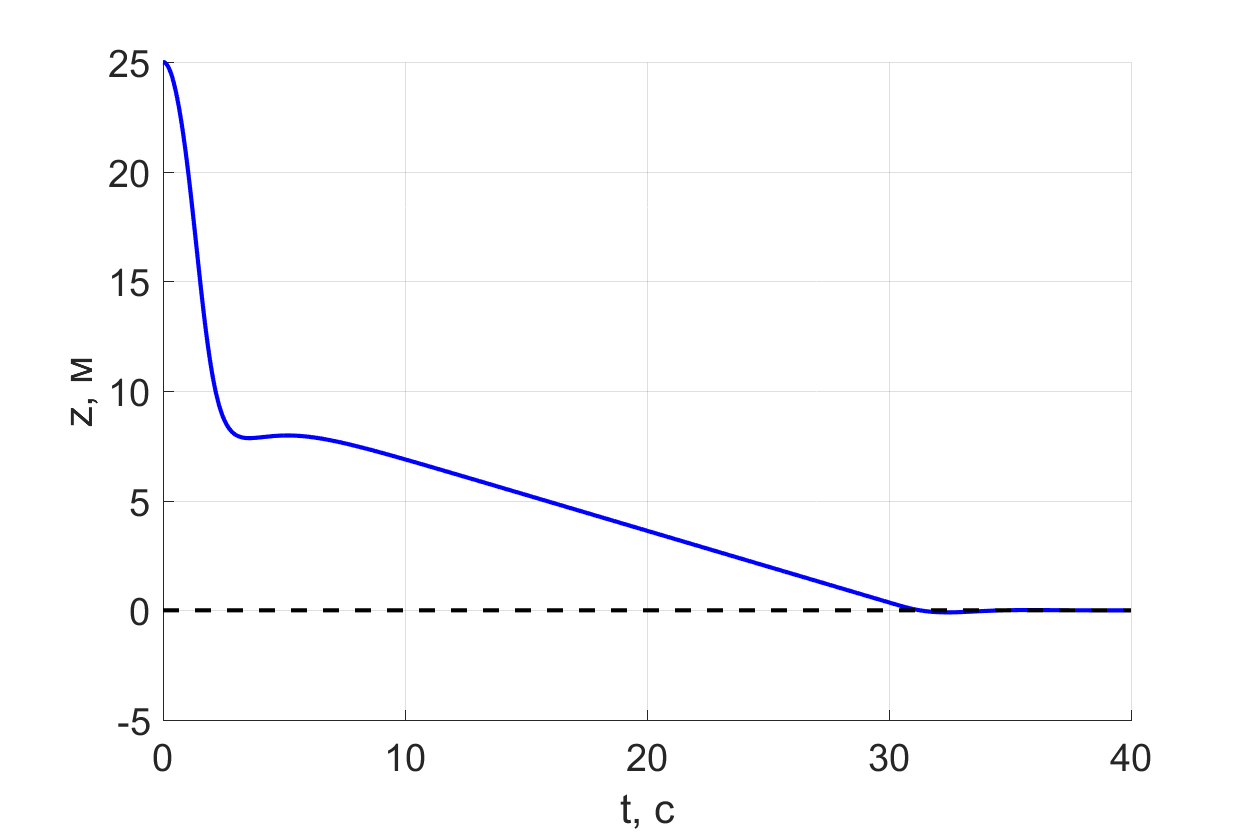
\includegraphics[width=8cm]{em/z}}
	\caption{ -- Параметры движения БЛА при экстренной посадке}
	\label{fig:em_coords}
\end{figure}

Таким образом показано, что БЛА с поворотными роторами при соблюдении некоторых требований к параметрам исполнительных органов системы управления способен продолжить свое движение после отказа двух смежных двигателей.
	\chapter{Заключение}
Основные результаты диссертации:
\begin{enumerate}
	\item Разработана математическая модель управляемой динамики квадрокоптера с поворотными роторами с учетом сил и моментов, действующих на все составные части системы;
	\item  Получено аналитическое решение задачи обратной динамики БЛА с поворотными роторами;
	\item Синтезирован контур управления квадрокоптером с поворотными роторами для независимого управления положением и ориентацией; 
	\item Разработан алгоритм для учета физических ограничений, накладываемых на исполнительные органы системы управления;
	\item Разработан алгоритм для идентификации основных параметров модели;
	\item Разработаны алгоритмы оценки состояния БЛА с поворотными роторами и проведен их сравнительный анализ.
	\item Разработаны алгоритмы экстренного управления квадрокоптером с поворотными роторами в случае отказа двух смежных двигателей.
\end{enumerate}
По результатам проведенного исследования можно сделать следующие
выводы:
\begin{enumerate}
	\item Расширение размерности вектора управляющих воздействий за счет применения сервоприводов, с помощью которых можно изменять направления тяги каждого из двигателей квадрокоптера, позволяет добиться независимого управления положением и ориентацией БЛА;
	\item Наличие аналитического решения задачи обратной динамики БЛА с поворотными роторами  позволяет ограничить каждую из компонент вектора управляющих воздействий с учетом технических возможностей исполнительных механизмов системы управления, что отражается на маневренных качествах БЛА;
	\item Конструкция квадрокоптера с поворотными роторами позволяет продолжить полет или осуществить безопасную посадку в случае выхода из строя одного или любой пары двигателей;
	\item Квадрокоптер с поворотными роторами способен выполнять задачу преследования подвижного объекта с его одновременным наблюдением с помощью жестко закрепленной на борту камеры.
\end{enumerate}
Таким образом, цели исследования, поставленные в диссертационной работе, достигнуты, и все
поставленные задачи – решены.
	\chapter*{Список сокращений и обозначений}
\addcontentsline{toc}{chapter}{Список сокращений и обозначений} 

\begin{tabular}{cl}
	БЛА -- & беспилотный летательный аппарат\\
	$I$ -- &система координат, связанная с землей\\
	$B$ -- &система координат, связанная с БЛА\\
	$R_i$ -- &система координат, связанная с землей\\
	$\bm r$ -- &положение БЛА\\
	$\bm v$ -- &скорость БЛА\\
	$q$ -- &кватернион ориентации БЛА\\
	$\bm \Omega$ -- &угловая скорость БЛА\\
	$L$ -- &расстояние от цетра масс до роторов БЛА\\
	$M$ -- &общая масса БЛА\\
	$\bm J_B$ -- &тензор инерции корпуса БЛА\\
	$\tilde \omega$ -- &обороты $i$-го двигателя БЛА\\
	$\theta$ -- &отклонение $i$-го сервопривода БЛА\\
	$k$ -- &аэродинамический коэффициент пропеллеров БЛА\\
	$b$ -- &аэродинамический коэффициент пропеллеров БЛА\\
	$C$ -- &аэродинамический коэффициент корпуса БЛА\\
	$\bm J_{R_i}$ -- &тензор инерции $i$-го ротора с пропеллером БЛА\\
	$\bm u$ -- &вектор управляющих воздействий\\
	$\bm x$ -- &вектор состояния БЛА\\
	$\bm z$ -- &вектор измерений БЛА\\
\end{tabular}
	\chapter*{Список работ автора}
\label{list_chapter}
\addcontentsline{toc}{chapter}{Список работ автора} 

\setlength{\parindent}{0mm}
\textbf{Публикации в изданиях, входящих в перечень ВАК:}

\begin{enumerate}
	\item Шавин, М. Ю. Управляемая динамика квадрокоптера с поворотными роторами. Инженерный журнал: наука и инновации, 2018, 76(4), doi: 10.18698/ 2308-6033-2018-4-1755.
	
	\item  Шавин М.Ю. Численные методы нелинейной фильтрации для оценки состояния квадрокоптера с   поворотными роторами // Труды МФТИ, 2019, 43(3): 86-95
\end{enumerate}
\textbf{Публикации в изданиях, входящих базу данных Scopus:}
\begin{enumerate}
	\item Shavin M. Design and identification of tilt-motor quadrotor control system //MATEC Web of Conferences. – EDP Sciences, 2018. – Т. 211. – С. 02013.
	
	\item  Шавин М.Ю., Притыкин Д.А. Синтез системы управления квадрокоптером с поворотными роторами и наблюдение за подвижной целью // Мехатроника, автоматизация, управление, 2019, 20(10):629-639, doi:\\ 10.17587/mau.20.629-639
\end{enumerate}

\textbf{Патенты и свидетельства:}
\begin{enumerate}
	\item Беспилотный летательный аппарат мультироторного типа. Полезная модель к патенту RU 183717 U1 //
	Автайкин М.В., Автайкин С.В., Буртелова Н.В.,
	Воронкин Д.А., Гильманов Х.Г., Залевский Д.Г.,
	Коротков Е.С., Макаров Н.Р., Нунупаров А.М.,
	Попов Л.Л., Карташов С.В., Скороход С.А,
	Тарасов М.В., Шавин М.Ю., Шкулов В.С. 2018 г.
	
	\item Программа расчета тяги двигателей квадрокоптера с поворотными роторами. Свидетельство о государственной регистрации программы для ЭВМ RU 2020611180 // Шавин Михаил Юрьевич. 2020 г.
	
	\item Программа локализации заданного объекта по изображениям с внешних камер. Свидетельство о государственной регистрации программы для ЭВМ RU 2020611181 // Шавин Николай Юрьевич, Шавин Михаил Юрьевич, Тарасов Максим Валерьевич. 2020 г.
	
	\item Программа калибровки положения внешних камер для системы слежения. Свидетельство о государственной регистрации программы для ЭВМ  RU 2020611113 // Шавин Михаил Юрьевич, Шавин Николай Юрьевич, Абдрашитов Артур Рашидович. 2020 г.
\end{enumerate}

\textbf{Публикации в других изданиях:}

\begin{enumerate}
	\item Шавин М. Ю. Динамика БПЛА с поворотными роторами // Всероссийская конференция молодых ученых-механиков: Тезисы докладов (5 - 15 сентября 2017 г., г. Сочи, «Буревестник» МГУ)  – М.: МГУ, 2017. с N-M. ISBN 978-5-19-011217-7
	
	\item Притыкин Д.А., Шавин М.Ю., Гильманов Х.Г. Управляемая динамика квадрокоптера с поворотными роторами // Международная научная конференция Фундаментальные и прикладные задачи механики: Тезисы докладов (24 - 27 октября 2017 г., г. Москва) / М.: Издательство МГТУ им. Н.Э. Баумана, 2017. с 94-95.
	ISBN 978-5-7038-4800-5
	
	\item Шавин М. Ю. Управляемая динамика беспилотного летательного аппарата (БПЛА) с поворотными роторами // Труды 60-й Всероссийской научной конференции МФТИ. Аэрокосмические технологии. Секция теоретической механики. (20–26 ноября 2017 г., г. Долгопрудный) -- М.: МФТИ, 2017. с 79. ISBN 978-5-7417-0646-6
	
	\item Шавин М. Ю. Управление беспилотным летательным аппаратом (БПЛА) с поворотными роторами // Труды 60-й Всероссийской научной конференции МФТИ. Аэрокосмические технологии. Секция управления динамическими системами. (20–26 ноября 2017 г., г. Долгопрудный) -- М.: МФТИ, 2017. с 23-24. ISBN 978-5-7417-0646-6
	
	\item Mikhail Yu. Shavin. Dynamics and Control of UAV with Variable Geometry // The Seventh International Conference «Geometry, Dynamics, Integrable Systems» – GDIS 2018: Book of Abstracts.
		
	\item Шавин М., Притыкин Д. Управляемая динамика квадрокоптера с поворотными роторами: алгоритмы оценки состояния // Проблемы механики и управления: Материалы международной конференции (16 - 22 сентября 2018 г., г. Махачкала) / ред. И.Г. Горячева – М.: Издательство Московского университета, 2018. с 337-339
	
\end{enumerate}

	\chapter*{Приложение А}
\label{A}
\addcontentsline{toc}{chapter}{Приложение А} 

Выражения для функций, входящих в уравнения обращенной динамики БЛА с поворотными роторами:
\begin{equation}
A_1 = (F_3kl + bF_2 - kT_2); \label{eq:app_solve_AB_begin}
\end{equation}
\begin{equation}
A_2 = (F_3kl + bF_1 + kT_1);
\end{equation}
\begin{equation}
A_3 = (F_3kl - bF_2 + kT_2);
\end{equation}
\begin{equation}
A_4 = (F_3kl - bF_1 - kT_1);
\end{equation}
\begin{equation}
B_1 = (bF_3 - kT_3 - F_2kl);
\end{equation}
\begin{equation}
B_2 = (bF_3 + kT_3 - F_1kl);
\end{equation}
\begin{equation}
B_3 = (bF_3 - kT_3 + F_2kl);
\end{equation}
\begin{equation}
B_4 = (bF_3 + kT_3 + F_1kl). \label{eq:app_solve_AB_end}
\end{equation}

Выражения для компонент вектора управляющих воздействий для обращенной динамики БЛА с двумя работающими двигателями: 

\begin{equation} \label{eq:app_em_solve_begin}
\begin{aligned}
&\tilde \omega_1 = \\&-\Big[2b^4F_1^2 + 4b^3F_1kT_2 + 4b^2F_1^2k^2l^2 - 2\sqrt{2}b^2F_1k^2lT_3 + 2b^2k^2T_2^2 + 4bF_1k^3l^2T_2 -\\ &-2\sqrt{2}bk^3lT_2T_3 + 2F_1^2k^4l^4 - 2\sqrt{2}F_1k^4l^3T_3 + 2k^4l^2T_1^2 - 4k^4l^2T_1T_2 + 2k^4l^2T_2^2 +\\ &+k^4l^2T_3^2 \Big]^{(0.5)} \Big(2k^2l(b^2 + k^2l^2)^{0.5)}\Big)^{-1};
\end{aligned}
\end{equation}

\begin{equation}
\begin{aligned}
&\tilde \omega_4 = \\&\Big[2b^4F_1^2 + 4b^3F_1kT_2 + 4b^2F_1^2k^2l^2 + 2\sqrt{2}b^2F_1k^2lT_3 + 2b^2k^2T_2^2 + 4bF_1k^3l^2T_2 + \\& +2\sqrt{2}bk^3lT_2T_3 + 2F_1^2k^4l^4 + 2\sqrt{2}F_1k^4l^3T_3 + 2k^4l^2T_1^2 + 4k^4l^2T_1T_2 + 2k^4l^2T_2^2 + \\& +k^4l^2T_3^2\Big]^{0.5} \Big(2k^2l(b^2 + k^2l^2)^{0.5}\Big)^{-1};
\end{aligned}
\end{equation}

\begin{equation}
\begin{aligned}
&\tilde \theta_1 = \\&2\text{arctg} \Big[\Big(2b^3F_1 - 2k^3l^2T_1 + 2k^3l^2T_2 + \sqrt{2}(b^2 + k^2l^2)^{0.5}
(2b^4F_1^2 + 4b^3F_1kT_2 +\\&+ 4b^2F_1^2k^2l^2 - 2\sqrt{2}b^2F_1k^2lT_3 + 2b^2k^2T_2^2 + 4bF_1k^3l^2T_2 - 2\sqrt{2}bk^3lT_2T_3 + 2F_1^2k^4l^4 - \\ -&2\sqrt{2}F_1k^4l^3T_3 + 2k^4l^2T_1^2 - 4k^4l^2T_1T_2 + 2k^4l^2T_2^2 + k^4l^2T_3^2)^{0.5} + 2b^2kT_2 + 2bF_1k^2l^2 - \\& -\sqrt{2}bk^2lT_3 \Big) \Big(kl(2F_1b^2 + 2T_1bk + 2F_1k^2l^2 - \sqrt{2}T_3k^2l)\Big)^{-1}\Big];
\end{aligned}
\end{equation}

\begin{equation} \label{eq:app_em_solve_end}
\begin{aligned}
&\tilde \theta_4 = \\&-2\text{arctg}\Big[\Big(2b^3F_1 + 2k^3l^2T_1 + 2k^3l^2T_2 + \sqrt{2}(b^2 + k^2l^2)^{0.5}(2b^4F_1^2 +  4b^3F_1kT_2  +\\& +4b^2F_1^2k^2l^2 + 2\sqrt{2}b^2F_1k^2lT_3 + 2b^2k^2T_2^2 + 4bF_1k^3l^2T_2 + 2\sqrt{2}bk^3lT_2T_3 + 2F_1^2k^4l^4 + \\& +2\sqrt{2}F_1k^4l^3T_3 + 2k^4l^2T_1^2 + 4k^4l^2T_1T_2 + 2k^4l^2T_2^2 + k^4l^2T_3^2)^{0.5} + 2b^2kT_2 + \\&+2bF_1k^2l^2 +\sqrt{2}bk^2lT_3\Big)\Big(kl(2F_1b^2 - 2T_1bk + 2F_1k^2l^2 + \sqrt{2}T_3k^2l)\Big)^{-1}\Big].
\end{aligned}
\end{equation}



	\sloppy
	\printbibliography
\end{document}


